\documentclass{book}
\usepackage[a4paper,top=2.5cm,bottom=2.5cm,left=2.5cm,right=2.5cm]{geometry}
\usepackage{makeidx}
\usepackage{natbib}
\usepackage{graphicx}
\usepackage{multicol}
\usepackage{float}
\usepackage{listings}
\usepackage{color}
\usepackage{ifthen}
\usepackage[table]{xcolor}
\usepackage{textcomp}
\usepackage{alltt}
\usepackage{ifpdf}
\ifpdf
\usepackage[pdftex,
            pagebackref=true,
            colorlinks=true,
            linkcolor=blue,
            unicode
           ]{hyperref}
\else
\usepackage[ps2pdf,
            pagebackref=true,
            colorlinks=true,
            linkcolor=blue,
            unicode
           ]{hyperref}
\usepackage{pspicture}
\fi
\usepackage[utf8]{inputenc}
\usepackage{mathptmx}
\usepackage[scaled=.90]{helvet}
\usepackage{courier}
\usepackage{sectsty}
\usepackage{amssymb}
\usepackage[titles]{tocloft}
\usepackage{doxygen}
\lstset{language=C++,inputencoding=utf8,basicstyle=\footnotesize,breaklines=true,breakatwhitespace=true,tabsize=4,numbers=left }
\makeindex
\setcounter{tocdepth}{3}
\renewcommand{\footrulewidth}{0.4pt}
\renewcommand{\familydefault}{\sfdefault}
\hfuzz=15pt
\setlength{\emergencystretch}{15pt}
\hbadness=750
\tolerance=750
\begin{document}
\hypersetup{pageanchor=false,citecolor=blue}
\begin{titlepage}
\vspace*{7cm}
\begin{center}
{\Large Le jeu 4 \\[1ex]\large v1.\-1 Ncurses }\\
\vspace*{1cm}
{\large Generated by Doxygen 1.8.3.1}\\
\vspace*{0.5cm}
{\small Tue Jan 6 2015 14:46:49}\\
\end{center}
\end{titlepage}
\clearemptydoublepage
\pagenumbering{roman}
\tableofcontents
\clearemptydoublepage
\pagenumbering{arabic}
\hypersetup{pageanchor=true,citecolor=blue}
\chapter{Readme}
\label{md_Readme}
\hypertarget{md_Readme}{}
Peut-\/être penser à la génération de terrain. Ca serait pas mal un ptit donjon avec des salles.

Configuration de Geany, cliquer sur le menu déroulant à côté de build, puis \char`\"{}définir les commandes de construction\char`\"{} puis \+:

\href{http://image.noelshack.com/fichiers/2014/51/1418816409-capture-du-2014-12-17-12-38-56.png}{\tt http\+://image.\+noelshack.\+com/fichiers/2014/51/1418816409-\/capture-\/du-\/2014-\/12-\/17-\/12-\/38-\/56.\+png} 
\chapter{Data Structure Index}
\section{Data Structures}
Here are the data structures with brief descriptions\-:\begin{DoxyCompactList}
\item\contentsline{section}{\hyperlink{structt__character}{t\-\_\-character} }{\pageref{structt__character}}{}
\item\contentsline{section}{\hyperlink{structt__coord}{t\-\_\-coord} }{\pageref{structt__coord}}{}
\item\contentsline{section}{\hyperlink{structt__player}{t\-\_\-player} }{\pageref{structt__player}}{}
\item\contentsline{section}{\hyperlink{structt__skill}{t\-\_\-skill} }{\pageref{structt__skill}}{}
\item\contentsline{section}{\hyperlink{structt__skill__list}{t\-\_\-skill\-\_\-list} }{\pageref{structt__skill__list}}{}
\item\contentsline{section}{\hyperlink{structt__stats}{t\-\_\-stats} }{\pageref{structt__stats}}{}
\item\contentsline{section}{\hyperlink{structt__status}{t\-\_\-status} }{\pageref{structt__status}}{}
\end{DoxyCompactList}

\chapter{File Index}
\section{Liste des fichiers}
Liste de tous les fichiers avec une brève description \-:\begin{DoxyCompactList}
\item\contentsline{section}{\hyperlink{file_8c}{file.\-c} }{\pageref{file_8c}}{}
\item\contentsline{section}{\hyperlink{file_8h}{file.\-h} }{\pageref{file_8h}}{}
\item\contentsline{section}{\hyperlink{header_8h}{header.\-h} \\*Header }{\pageref{header_8h}}{}
\item\contentsline{section}{\hyperlink{liste_8c}{liste.\-c} }{\pageref{liste_8c}}{}
\item\contentsline{section}{\hyperlink{liste_8h}{liste.\-h} }{\pageref{liste_8h}}{}
\item\contentsline{section}{\hyperlink{_minimale_8c}{Minimale.\-c} \\*Code principal }{\pageref{_minimale_8c}}{}
\item\contentsline{section}{\hyperlink{pile_8c}{pile.\-c} \\*Projet informatique S3 Deplacement du personnage et colisions sur le parois }{\pageref{pile_8c}}{}
\item\contentsline{section}{\hyperlink{pile_8h}{pile.\-h} }{\pageref{pile_8h}}{}
\end{DoxyCompactList}

\chapter{Data Structure Documentation}
\hypertarget{structt__character}{\section{t\-\_\-character Struct Reference}
\label{structt__character}\index{t\-\_\-character@{t\-\_\-character}}
}


{\ttfamily \#include $<$header.\-h$>$}



Collaboration diagram for t\-\_\-character\-:\nopagebreak
\begin{figure}[H]
\begin{center}
\leavevmode
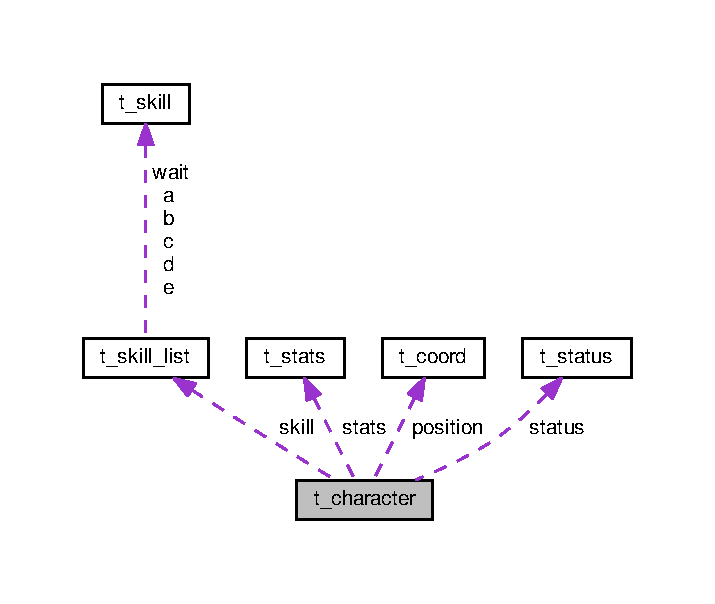
\includegraphics[width=343pt]{structt__character__coll__graph}
\end{center}
\end{figure}
\subsection*{Data Fields}
\begin{DoxyCompactItemize}
\item 
char \hyperlink{structt__character_ab27f28c5ead39031421706ddbbd1edea}{name} \mbox{[}\hyperlink{header_8h_ab154998a3a376095f3601bc35c5cf523}{Max\-String}\mbox{]}
\item 
\hyperlink{structt__coord}{t\-\_\-coord} \hyperlink{structt__character_a27c93348dcaa3ea78282fb5ef6ce371b}{position}
\item 
\hyperlink{header_8h_a6dc6eccccaf78ef029cff998c0e654f4}{t\-\_\-orientation} \hyperlink{structt__character_af778044107ad1a59b9725fa3962560ad}{orientation}
\item 
\hyperlink{structt__status}{t\-\_\-status} \hyperlink{structt__character_a3ade6b90793e915ca28b52fb70e58e3f}{status}
\item 
\hyperlink{structt__stats}{t\-\_\-stats} \hyperlink{structt__character_a29711825af64d428d19df366a5056670}{stats}
\item 
\hyperlink{structt__skill__list}{t\-\_\-skill\-\_\-list} \hyperlink{structt__character_ae7aa14804e69b1bc9652c16261da0c9f}{skill}
\item 
\hyperlink{header_8h_a4bb25c9352f7bb2ea2eb663ccf579528}{t\-\_\-camp} \hyperlink{structt__character_a48707185be865bad67e5c61e5903ae5a}{camp}
\item 
int \hyperlink{structt__character_aaff424b51f4bd3db2c199cc08f21f86d}{nb\-\_\-action\-\_\-tour}
\item 
\hyperlink{header_8h_ac8020d257c824e4b188c04ee386ebfda}{t\-\_\-character\-\_\-type} \hyperlink{structt__character_a3b5fecb9824668aab778f82005089942}{type}
\end{DoxyCompactItemize}


\subsection{Field Documentation}
\hypertarget{structt__character_a48707185be865bad67e5c61e5903ae5a}{\index{t\-\_\-character@{t\-\_\-character}!camp@{camp}}
\index{camp@{camp}!t_character@{t\-\_\-character}}
\subsubsection[{camp}]{\setlength{\rightskip}{0pt plus 5cm}{\bf t\-\_\-camp} camp}}\label{structt__character_a48707185be865bad67e5c61e5903ae5a}
\hypertarget{structt__character_ab27f28c5ead39031421706ddbbd1edea}{\index{t\-\_\-character@{t\-\_\-character}!name@{name}}
\index{name@{name}!t_character@{t\-\_\-character}}
\subsubsection[{name}]{\setlength{\rightskip}{0pt plus 5cm}char name\mbox{[}{\bf Max\-String}\mbox{]}}}\label{structt__character_ab27f28c5ead39031421706ddbbd1edea}
\hypertarget{structt__character_aaff424b51f4bd3db2c199cc08f21f86d}{\index{t\-\_\-character@{t\-\_\-character}!nb\-\_\-action\-\_\-tour@{nb\-\_\-action\-\_\-tour}}
\index{nb\-\_\-action\-\_\-tour@{nb\-\_\-action\-\_\-tour}!t_character@{t\-\_\-character}}
\subsubsection[{nb\-\_\-action\-\_\-tour}]{\setlength{\rightskip}{0pt plus 5cm}int nb\-\_\-action\-\_\-tour}}\label{structt__character_aaff424b51f4bd3db2c199cc08f21f86d}
\hypertarget{structt__character_af778044107ad1a59b9725fa3962560ad}{\index{t\-\_\-character@{t\-\_\-character}!orientation@{orientation}}
\index{orientation@{orientation}!t_character@{t\-\_\-character}}
\subsubsection[{orientation}]{\setlength{\rightskip}{0pt plus 5cm}{\bf t\-\_\-orientation} orientation}}\label{structt__character_af778044107ad1a59b9725fa3962560ad}
\hypertarget{structt__character_a27c93348dcaa3ea78282fb5ef6ce371b}{\index{t\-\_\-character@{t\-\_\-character}!position@{position}}
\index{position@{position}!t_character@{t\-\_\-character}}
\subsubsection[{position}]{\setlength{\rightskip}{0pt plus 5cm}{\bf t\-\_\-coord} position}}\label{structt__character_a27c93348dcaa3ea78282fb5ef6ce371b}
\hypertarget{structt__character_ae7aa14804e69b1bc9652c16261da0c9f}{\index{t\-\_\-character@{t\-\_\-character}!skill@{skill}}
\index{skill@{skill}!t_character@{t\-\_\-character}}
\subsubsection[{skill}]{\setlength{\rightskip}{0pt plus 5cm}{\bf t\-\_\-skill\-\_\-list} skill}}\label{structt__character_ae7aa14804e69b1bc9652c16261da0c9f}
\hypertarget{structt__character_a29711825af64d428d19df366a5056670}{\index{t\-\_\-character@{t\-\_\-character}!stats@{stats}}
\index{stats@{stats}!t_character@{t\-\_\-character}}
\subsubsection[{stats}]{\setlength{\rightskip}{0pt plus 5cm}{\bf t\-\_\-stats} stats}}\label{structt__character_a29711825af64d428d19df366a5056670}
\hypertarget{structt__character_a3ade6b90793e915ca28b52fb70e58e3f}{\index{t\-\_\-character@{t\-\_\-character}!status@{status}}
\index{status@{status}!t_character@{t\-\_\-character}}
\subsubsection[{status}]{\setlength{\rightskip}{0pt plus 5cm}{\bf t\-\_\-status} status}}\label{structt__character_a3ade6b90793e915ca28b52fb70e58e3f}
\hypertarget{structt__character_a3b5fecb9824668aab778f82005089942}{\index{t\-\_\-character@{t\-\_\-character}!type@{type}}
\index{type@{type}!t_character@{t\-\_\-character}}
\subsubsection[{type}]{\setlength{\rightskip}{0pt plus 5cm}{\bf t\-\_\-character\-\_\-type} type}}\label{structt__character_a3b5fecb9824668aab778f82005089942}


The documentation for this struct was generated from the following file\-:\begin{DoxyCompactItemize}
\item 
\hyperlink{header_8h}{header.\-h}\end{DoxyCompactItemize}

\hypertarget{structt__coord}{\section{Référence de la structure t\+\_\+coord}
\label{structt__coord}\index{t\+\_\+coord@{t\+\_\+coord}}
}


{\ttfamily \#include $<$header.\+h$>$}

\subsection*{Champs de données}
\begin{DoxyCompactItemize}
\item 
int \hyperlink{structt__coord_a80c0944640e62d3ed6c5419c1bcc0c88}{X}
\item 
int \hyperlink{structt__coord_aa482c4cc86a24474e4fb19b5b5978778}{Y}
\end{DoxyCompactItemize}


\subsection{Description détaillée}


Définition à la ligne 81 du fichier header.\+h.



\subsection{Documentation des champs}
\hypertarget{structt__coord_a80c0944640e62d3ed6c5419c1bcc0c88}{\index{t\+\_\+coord@{t\+\_\+coord}!X@{X}}
\index{X@{X}!t\+\_\+coord@{t\+\_\+coord}}
\subsubsection[{X}]{\setlength{\rightskip}{0pt plus 5cm}int X}}\label{structt__coord_a80c0944640e62d3ed6c5419c1bcc0c88}


Définition à la ligne 81 du fichier header.\+h.

\hypertarget{structt__coord_aa482c4cc86a24474e4fb19b5b5978778}{\index{t\+\_\+coord@{t\+\_\+coord}!Y@{Y}}
\index{Y@{Y}!t\+\_\+coord@{t\+\_\+coord}}
\subsubsection[{Y}]{\setlength{\rightskip}{0pt plus 5cm}int Y}}\label{structt__coord_aa482c4cc86a24474e4fb19b5b5978778}


Définition à la ligne 81 du fichier header.\+h.



La documentation de cette structure a été générée à partir du fichier suivant \+:\begin{DoxyCompactItemize}
\item 
\hyperlink{header_8h}{header.\+h}\end{DoxyCompactItemize}

\hypertarget{structt__player}{\section{t\-\_\-player Struct Reference}
\label{structt__player}\index{t\-\_\-player@{t\-\_\-player}}
}


{\ttfamily \#include $<$header.\-h$>$}

\subsection*{Data Fields}
\begin{DoxyCompactItemize}
\item 
int \hyperlink{structt__player_afaea7716a081e71f804e80c2d5a92390}{alive}
\item 
char \hyperlink{structt__player_ab27f28c5ead39031421706ddbbd1edea}{name} \mbox{[}\hyperlink{header_8h_ab154998a3a376095f3601bc35c5cf523}{Max\-String}\mbox{]}
\end{DoxyCompactItemize}


\subsection{Detailed Description}


Definition at line 44 of file header.\-h.



\subsection{Field Documentation}
\hypertarget{structt__player_afaea7716a081e71f804e80c2d5a92390}{\index{t\-\_\-player@{t\-\_\-player}!alive@{alive}}
\index{alive@{alive}!t_player@{t\-\_\-player}}
\subsubsection[{alive}]{\setlength{\rightskip}{0pt plus 5cm}int alive}}\label{structt__player_afaea7716a081e71f804e80c2d5a92390}


Definition at line 44 of file header.\-h.

\hypertarget{structt__player_ab27f28c5ead39031421706ddbbd1edea}{\index{t\-\_\-player@{t\-\_\-player}!name@{name}}
\index{name@{name}!t_player@{t\-\_\-player}}
\subsubsection[{name}]{\setlength{\rightskip}{0pt plus 5cm}char name\mbox{[}{\bf Max\-String}\mbox{]}}}\label{structt__player_ab27f28c5ead39031421706ddbbd1edea}


Definition at line 44 of file header.\-h.



The documentation for this struct was generated from the following file\-:\begin{DoxyCompactItemize}
\item 
\hyperlink{header_8h}{header.\-h}\end{DoxyCompactItemize}

\hypertarget{structt__skill}{\section{Référence de la structure t\+\_\+skill}
\label{structt__skill}\index{t\+\_\+skill@{t\+\_\+skill}}
}


{\ttfamily \#include $<$header.\+h$>$}

\subsection*{Champs de données}
\begin{DoxyCompactItemize}
\item 
char \hyperlink{structt__skill_ab27f28c5ead39031421706ddbbd1edea}{name} \mbox{[}\hyperlink{header_8h_ab154998a3a376095f3601bc35c5cf523}{Max\+String}\mbox{]}
\item 
int \hyperlink{structt__skill_a037e8e370380046bec287bdc96942091}{range}
\item 
\hyperlink{header_8h_a440f669d36bc2028077af38574051204}{t\+\_\+skilltype} \hyperlink{structt__skill_ac00edc3c188c78c47878a357ecff2954}{type}
\item 
int \hyperlink{structt__skill_a9518a5f7d916a01def3588da5dc0c8fa}{damage\+\_\+coeff}
\end{DoxyCompactItemize}


\subsection{Description détaillée}


Définition à la ligne 82 du fichier header.\+h.



\subsection{Documentation des champs}
\hypertarget{structt__skill_a9518a5f7d916a01def3588da5dc0c8fa}{\index{t\+\_\+skill@{t\+\_\+skill}!damage\+\_\+coeff@{damage\+\_\+coeff}}
\index{damage\+\_\+coeff@{damage\+\_\+coeff}!t\+\_\+skill@{t\+\_\+skill}}
\subsubsection[{damage\+\_\+coeff}]{\setlength{\rightskip}{0pt plus 5cm}int damage\+\_\+coeff}}\label{structt__skill_a9518a5f7d916a01def3588da5dc0c8fa}


Définition à la ligne 82 du fichier header.\+h.

\hypertarget{structt__skill_ab27f28c5ead39031421706ddbbd1edea}{\index{t\+\_\+skill@{t\+\_\+skill}!name@{name}}
\index{name@{name}!t\+\_\+skill@{t\+\_\+skill}}
\subsubsection[{name}]{\setlength{\rightskip}{0pt plus 5cm}char name\mbox{[}{\bf Max\+String}\mbox{]}}}\label{structt__skill_ab27f28c5ead39031421706ddbbd1edea}


Définition à la ligne 82 du fichier header.\+h.

\hypertarget{structt__skill_a037e8e370380046bec287bdc96942091}{\index{t\+\_\+skill@{t\+\_\+skill}!range@{range}}
\index{range@{range}!t\+\_\+skill@{t\+\_\+skill}}
\subsubsection[{range}]{\setlength{\rightskip}{0pt plus 5cm}int range}}\label{structt__skill_a037e8e370380046bec287bdc96942091}


Définition à la ligne 82 du fichier header.\+h.

\hypertarget{structt__skill_ac00edc3c188c78c47878a357ecff2954}{\index{t\+\_\+skill@{t\+\_\+skill}!type@{type}}
\index{type@{type}!t\+\_\+skill@{t\+\_\+skill}}
\subsubsection[{type}]{\setlength{\rightskip}{0pt plus 5cm}{\bf t\+\_\+skilltype} type}}\label{structt__skill_ac00edc3c188c78c47878a357ecff2954}


Définition à la ligne 82 du fichier header.\+h.



La documentation de cette structure a été générée à partir du fichier suivant \+:\begin{DoxyCompactItemize}
\item 
\hyperlink{header_8h}{header.\+h}\end{DoxyCompactItemize}

\hypertarget{structt__skill__list}{\section{Référence de la structure t\+\_\+skill\+\_\+list}
\label{structt__skill__list}\index{t\+\_\+skill\+\_\+list@{t\+\_\+skill\+\_\+list}}
}


{\ttfamily \#include $<$header.\+h$>$}



Graphe de collaboration de t\+\_\+skill\+\_\+list\+:
\nopagebreak
\begin{figure}[H]
\begin{center}
\leavevmode
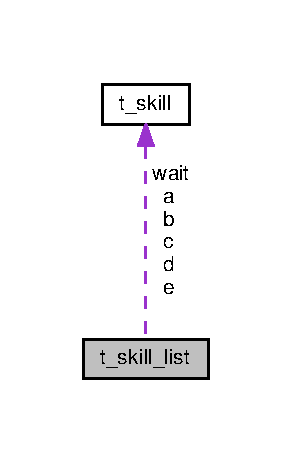
\includegraphics[width=140pt]{structt__skill__list__coll__graph}
\end{center}
\end{figure}
\subsection*{Champs de données}
\begin{DoxyCompactItemize}
\item 
\hyperlink{structt__skill}{t\+\_\+skill} \hyperlink{structt__skill__list_a39a494bb9ce01ba13ea4577fe2b1cc79}{a}
\item 
\hyperlink{structt__skill}{t\+\_\+skill} \hyperlink{structt__skill__list_a85ae40dbaecefd131b936ec65e9f4809}{b}
\item 
\hyperlink{structt__skill}{t\+\_\+skill} \hyperlink{structt__skill__list_ac9055dd2d5c45c223e3b0e1920c31493}{c}
\item 
\hyperlink{structt__skill}{t\+\_\+skill} \hyperlink{structt__skill__list_a0bb2c4a26ff65aecd7a36ad7ee898cd8}{d}
\item 
\hyperlink{structt__skill}{t\+\_\+skill} \hyperlink{structt__skill__list_aa756d3dbc91762775cff0f4b52526a70}{e}
\item 
\hyperlink{structt__skill}{t\+\_\+skill} \hyperlink{structt__skill__list_a2a4af1a4acb8da6061990f9bd8d0a564}{wait}
\end{DoxyCompactItemize}


\subsection{Description détaillée}


Définition à la ligne 83 du fichier header.\+h.



\subsection{Documentation des champs}
\hypertarget{structt__skill__list_a39a494bb9ce01ba13ea4577fe2b1cc79}{\index{t\+\_\+skill\+\_\+list@{t\+\_\+skill\+\_\+list}!a@{a}}
\index{a@{a}!t\+\_\+skill\+\_\+list@{t\+\_\+skill\+\_\+list}}
\subsubsection[{a}]{\setlength{\rightskip}{0pt plus 5cm}{\bf t\+\_\+skill} a}}\label{structt__skill__list_a39a494bb9ce01ba13ea4577fe2b1cc79}


Définition à la ligne 83 du fichier header.\+h.

\hypertarget{structt__skill__list_a85ae40dbaecefd131b936ec65e9f4809}{\index{t\+\_\+skill\+\_\+list@{t\+\_\+skill\+\_\+list}!b@{b}}
\index{b@{b}!t\+\_\+skill\+\_\+list@{t\+\_\+skill\+\_\+list}}
\subsubsection[{b}]{\setlength{\rightskip}{0pt plus 5cm}{\bf t\+\_\+skill} b}}\label{structt__skill__list_a85ae40dbaecefd131b936ec65e9f4809}


Définition à la ligne 83 du fichier header.\+h.

\hypertarget{structt__skill__list_ac9055dd2d5c45c223e3b0e1920c31493}{\index{t\+\_\+skill\+\_\+list@{t\+\_\+skill\+\_\+list}!c@{c}}
\index{c@{c}!t\+\_\+skill\+\_\+list@{t\+\_\+skill\+\_\+list}}
\subsubsection[{c}]{\setlength{\rightskip}{0pt plus 5cm}{\bf t\+\_\+skill} c}}\label{structt__skill__list_ac9055dd2d5c45c223e3b0e1920c31493}


Définition à la ligne 83 du fichier header.\+h.

\hypertarget{structt__skill__list_a0bb2c4a26ff65aecd7a36ad7ee898cd8}{\index{t\+\_\+skill\+\_\+list@{t\+\_\+skill\+\_\+list}!d@{d}}
\index{d@{d}!t\+\_\+skill\+\_\+list@{t\+\_\+skill\+\_\+list}}
\subsubsection[{d}]{\setlength{\rightskip}{0pt plus 5cm}{\bf t\+\_\+skill} d}}\label{structt__skill__list_a0bb2c4a26ff65aecd7a36ad7ee898cd8}


Définition à la ligne 83 du fichier header.\+h.

\hypertarget{structt__skill__list_aa756d3dbc91762775cff0f4b52526a70}{\index{t\+\_\+skill\+\_\+list@{t\+\_\+skill\+\_\+list}!e@{e}}
\index{e@{e}!t\+\_\+skill\+\_\+list@{t\+\_\+skill\+\_\+list}}
\subsubsection[{e}]{\setlength{\rightskip}{0pt plus 5cm}{\bf t\+\_\+skill} e}}\label{structt__skill__list_aa756d3dbc91762775cff0f4b52526a70}


Définition à la ligne 83 du fichier header.\+h.

\hypertarget{structt__skill__list_a2a4af1a4acb8da6061990f9bd8d0a564}{\index{t\+\_\+skill\+\_\+list@{t\+\_\+skill\+\_\+list}!wait@{wait}}
\index{wait@{wait}!t\+\_\+skill\+\_\+list@{t\+\_\+skill\+\_\+list}}
\subsubsection[{wait}]{\setlength{\rightskip}{0pt plus 5cm}{\bf t\+\_\+skill} wait}}\label{structt__skill__list_a2a4af1a4acb8da6061990f9bd8d0a564}


Définition à la ligne 83 du fichier header.\+h.



La documentation de cette structure a été générée à partir du fichier suivant \+:\begin{DoxyCompactItemize}
\item 
\hyperlink{header_8h}{header.\+h}\end{DoxyCompactItemize}

\hypertarget{structt__stats}{\section{t\-\_\-stats Struct Reference}
\label{structt__stats}\index{t\-\_\-stats@{t\-\_\-stats}}
}


{\ttfamily \#include $<$header.\-h$>$}

\subsection*{Data Fields}
\begin{DoxyCompactItemize}
\item 
int \hyperlink{structt__stats_a3b3918526788ae6b163c41dc25326396}{A\-T\-K}
\item 
int \hyperlink{structt__stats_ae183b98dc9aca9905f531bfd4dd51a1c}{M\-A\-T\-K}
\item 
int \hyperlink{structt__stats_a30707041436614e9e3759b7bf533b201}{D\-E\-F}
\item 
int \hyperlink{structt__stats_a92ab6d75a95ed209b7875314f53fb555}{M\-D\-E\-F}
\item 
int \hyperlink{structt__stats_a397f7940443939415a50f324dc5f56f9}{M\-V\-T}
\end{DoxyCompactItemize}


\subsection{Detailed Description}


Definition at line 37 of file header.\-h.



\subsection{Field Documentation}
\hypertarget{structt__stats_a3b3918526788ae6b163c41dc25326396}{\index{t\-\_\-stats@{t\-\_\-stats}!A\-T\-K@{A\-T\-K}}
\index{A\-T\-K@{A\-T\-K}!t_stats@{t\-\_\-stats}}
\subsubsection[{A\-T\-K}]{\setlength{\rightskip}{0pt plus 5cm}int A\-T\-K}}\label{structt__stats_a3b3918526788ae6b163c41dc25326396}


Definition at line 37 of file header.\-h.

\hypertarget{structt__stats_a30707041436614e9e3759b7bf533b201}{\index{t\-\_\-stats@{t\-\_\-stats}!D\-E\-F@{D\-E\-F}}
\index{D\-E\-F@{D\-E\-F}!t_stats@{t\-\_\-stats}}
\subsubsection[{D\-E\-F}]{\setlength{\rightskip}{0pt plus 5cm}int D\-E\-F}}\label{structt__stats_a30707041436614e9e3759b7bf533b201}


Definition at line 37 of file header.\-h.

\hypertarget{structt__stats_ae183b98dc9aca9905f531bfd4dd51a1c}{\index{t\-\_\-stats@{t\-\_\-stats}!M\-A\-T\-K@{M\-A\-T\-K}}
\index{M\-A\-T\-K@{M\-A\-T\-K}!t_stats@{t\-\_\-stats}}
\subsubsection[{M\-A\-T\-K}]{\setlength{\rightskip}{0pt plus 5cm}int M\-A\-T\-K}}\label{structt__stats_ae183b98dc9aca9905f531bfd4dd51a1c}


Definition at line 37 of file header.\-h.

\hypertarget{structt__stats_a92ab6d75a95ed209b7875314f53fb555}{\index{t\-\_\-stats@{t\-\_\-stats}!M\-D\-E\-F@{M\-D\-E\-F}}
\index{M\-D\-E\-F@{M\-D\-E\-F}!t_stats@{t\-\_\-stats}}
\subsubsection[{M\-D\-E\-F}]{\setlength{\rightskip}{0pt plus 5cm}int M\-D\-E\-F}}\label{structt__stats_a92ab6d75a95ed209b7875314f53fb555}


Definition at line 37 of file header.\-h.

\hypertarget{structt__stats_a397f7940443939415a50f324dc5f56f9}{\index{t\-\_\-stats@{t\-\_\-stats}!M\-V\-T@{M\-V\-T}}
\index{M\-V\-T@{M\-V\-T}!t_stats@{t\-\_\-stats}}
\subsubsection[{M\-V\-T}]{\setlength{\rightskip}{0pt plus 5cm}int M\-V\-T}}\label{structt__stats_a397f7940443939415a50f324dc5f56f9}


Definition at line 37 of file header.\-h.



The documentation for this struct was generated from the following file\-:\begin{DoxyCompactItemize}
\item 
\hyperlink{header_8h}{header.\-h}\end{DoxyCompactItemize}

\hypertarget{structt__status}{\section{Référence de la structure t\-\_\-status}
\label{structt__status}\index{t\-\_\-status@{t\-\_\-status}}
}


{\ttfamily \#include $<$header.\-h$>$}

\subsection*{Champs de données}
\begin{DoxyCompactItemize}
\item 
int \hyperlink{structt__status_a58ca25ca6c9448a364b84539e42f1fa6}{H\-P}
\item 
int \hyperlink{structt__status_a3ae8966f5c827b3c74072acda8de72af}{Max\-\_\-\-H\-P}
\item 
int \hyperlink{structt__status_a30fc75b90111fc791752dd1add6ed991}{M\-P}
\item 
int \hyperlink{structt__status_a5e48a681ff3d92aaa0e643fbc32ab2f7}{Max\-\_\-\-M\-P}
\end{DoxyCompactItemize}


\subsection{Description détaillée}


Définition à la ligne 79 du fichier header.\-h.



\subsection{Documentation des champs}
\hypertarget{structt__status_a58ca25ca6c9448a364b84539e42f1fa6}{\index{t\-\_\-status@{t\-\_\-status}!H\-P@{H\-P}}
\index{H\-P@{H\-P}!t_status@{t\-\_\-status}}
\subsubsection[{H\-P}]{\setlength{\rightskip}{0pt plus 5cm}int H\-P}}\label{structt__status_a58ca25ca6c9448a364b84539e42f1fa6}


Définition à la ligne 79 du fichier header.\-h.

\hypertarget{structt__status_a3ae8966f5c827b3c74072acda8de72af}{\index{t\-\_\-status@{t\-\_\-status}!Max\-\_\-\-H\-P@{Max\-\_\-\-H\-P}}
\index{Max\-\_\-\-H\-P@{Max\-\_\-\-H\-P}!t_status@{t\-\_\-status}}
\subsubsection[{Max\-\_\-\-H\-P}]{\setlength{\rightskip}{0pt plus 5cm}int Max\-\_\-\-H\-P}}\label{structt__status_a3ae8966f5c827b3c74072acda8de72af}


Définition à la ligne 79 du fichier header.\-h.

\hypertarget{structt__status_a5e48a681ff3d92aaa0e643fbc32ab2f7}{\index{t\-\_\-status@{t\-\_\-status}!Max\-\_\-\-M\-P@{Max\-\_\-\-M\-P}}
\index{Max\-\_\-\-M\-P@{Max\-\_\-\-M\-P}!t_status@{t\-\_\-status}}
\subsubsection[{Max\-\_\-\-M\-P}]{\setlength{\rightskip}{0pt plus 5cm}int Max\-\_\-\-M\-P}}\label{structt__status_a5e48a681ff3d92aaa0e643fbc32ab2f7}


Définition à la ligne 79 du fichier header.\-h.

\hypertarget{structt__status_a30fc75b90111fc791752dd1add6ed991}{\index{t\-\_\-status@{t\-\_\-status}!M\-P@{M\-P}}
\index{M\-P@{M\-P}!t_status@{t\-\_\-status}}
\subsubsection[{M\-P}]{\setlength{\rightskip}{0pt plus 5cm}int M\-P}}\label{structt__status_a30fc75b90111fc791752dd1add6ed991}


Définition à la ligne 79 du fichier header.\-h.



La documentation de cette structure a été générée à partir du fichier suivant \-:\begin{DoxyCompactItemize}
\item 
\hyperlink{header_8h}{header.\-h}\end{DoxyCompactItemize}

\chapter{File Documentation}
\hypertarget{file_8c}{\section{Référence du fichier file.\-c}
\label{file_8c}\index{file.\-c@{file.\-c}}
}
{\ttfamily \#include \char`\"{}file.\-h\char`\"{}}\\*
{\ttfamily \#include \char`\"{}header.\-h\char`\"{}}\\*
{\ttfamily \#include $<$stdio.\-h$>$}\\*
Graphe des dépendances par inclusion de file.\-c\-:\nopagebreak
\begin{figure}[H]
\begin{center}
\leavevmode
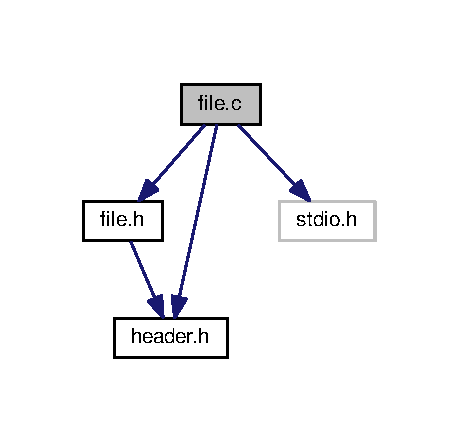
\includegraphics[width=220pt]{file_8c__incl}
\end{center}
\end{figure}
\subsection*{Macros}
\begin{DoxyCompactItemize}
\item 
\#define \hyperlink{file_8c_af7a16e2716eaac90fb331c55876cf511}{T\-M\-A\-X}~100
\end{DoxyCompactItemize}
\subsection*{Fonctions}
\begin{DoxyCompactItemize}
\item 
void \hyperlink{file_8c_a004123a6f8cce9d4168b0ea8cfdf133a}{file\-\_\-init} ()
\item 
void \hyperlink{file_8c_a9a4198b0c69187d42420b80f3e5b8d62}{file\-\_\-ajouter} (\hyperlink{structt__coord}{t\-\_\-coord} a)
\item 
void \hyperlink{file_8c_a59173755d515eb366fb01dba42a73e8e}{file\-\_\-retirer} (\hyperlink{structt__coord}{t\-\_\-coord} $\ast$val)
\item 
int \hyperlink{file_8c_a30c4f88a35783c4832434e9676ad98f5}{file\-\_\-vide} ()
\item 
void \hyperlink{file_8c_a141d57004b90128d46274ba60f61249f}{file\-\_\-liste\-\_\-afficher\-\_\-queue} ()
\item 
void \hyperlink{file_8c_a96c6e33606180f008c28906ff16f873a}{file\-\_\-afficher\-\_\-elt} (\hyperlink{structt__coord}{t\-\_\-coord} val)
\end{DoxyCompactItemize}


\subsection{Documentation des macros}
\hypertarget{file_8c_af7a16e2716eaac90fb331c55876cf511}{\index{file.\-c@{file.\-c}!T\-M\-A\-X@{T\-M\-A\-X}}
\index{T\-M\-A\-X@{T\-M\-A\-X}!file.c@{file.\-c}}
\subsubsection[{T\-M\-A\-X}]{\setlength{\rightskip}{0pt plus 5cm}\#define T\-M\-A\-X~100}}\label{file_8c_af7a16e2716eaac90fb331c55876cf511}


Définition à la ligne 4 du fichier file.\-c.



\subsection{Documentation des fonctions}
\hypertarget{file_8c_a96c6e33606180f008c28906ff16f873a}{\index{file.\-c@{file.\-c}!file\-\_\-afficher\-\_\-elt@{file\-\_\-afficher\-\_\-elt}}
\index{file\-\_\-afficher\-\_\-elt@{file\-\_\-afficher\-\_\-elt}!file.c@{file.\-c}}
\subsubsection[{file\-\_\-afficher\-\_\-elt}]{\setlength{\rightskip}{0pt plus 5cm}void file\-\_\-afficher\-\_\-elt (
\begin{DoxyParamCaption}
\item[{{\bf t\-\_\-coord}}]{val}
\end{DoxyParamCaption}
)}}\label{file_8c_a96c6e33606180f008c28906ff16f873a}


Définition à la ligne 53 du fichier file.\-c.

\hypertarget{file_8c_a9a4198b0c69187d42420b80f3e5b8d62}{\index{file.\-c@{file.\-c}!file\-\_\-ajouter@{file\-\_\-ajouter}}
\index{file\-\_\-ajouter@{file\-\_\-ajouter}!file.c@{file.\-c}}
\subsubsection[{file\-\_\-ajouter}]{\setlength{\rightskip}{0pt plus 5cm}void file\-\_\-ajouter (
\begin{DoxyParamCaption}
\item[{{\bf t\-\_\-coord}}]{a}
\end{DoxyParamCaption}
)}}\label{file_8c_a9a4198b0c69187d42420b80f3e5b8d62}


Définition à la ligne 16 du fichier file.\-c.



Voici le graphe des appelants de cette fonction \-:\nopagebreak
\begin{figure}[H]
\begin{center}
\leavevmode
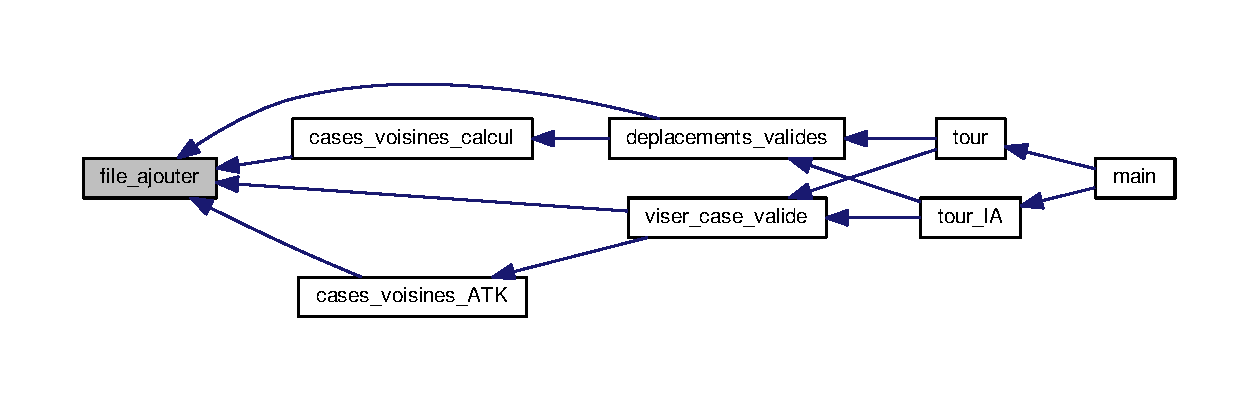
\includegraphics[width=350pt]{file_8c_a9a4198b0c69187d42420b80f3e5b8d62_icgraph}
\end{center}
\end{figure}


\hypertarget{file_8c_a004123a6f8cce9d4168b0ea8cfdf133a}{\index{file.\-c@{file.\-c}!file\-\_\-init@{file\-\_\-init}}
\index{file\-\_\-init@{file\-\_\-init}!file.c@{file.\-c}}
\subsubsection[{file\-\_\-init}]{\setlength{\rightskip}{0pt plus 5cm}void file\-\_\-init (
\begin{DoxyParamCaption}
{}
\end{DoxyParamCaption}
)}}\label{file_8c_a004123a6f8cce9d4168b0ea8cfdf133a}


Définition à la ligne 8 du fichier file.\-c.



Voici le graphe des appelants de cette fonction \-:\nopagebreak
\begin{figure}[H]
\begin{center}
\leavevmode
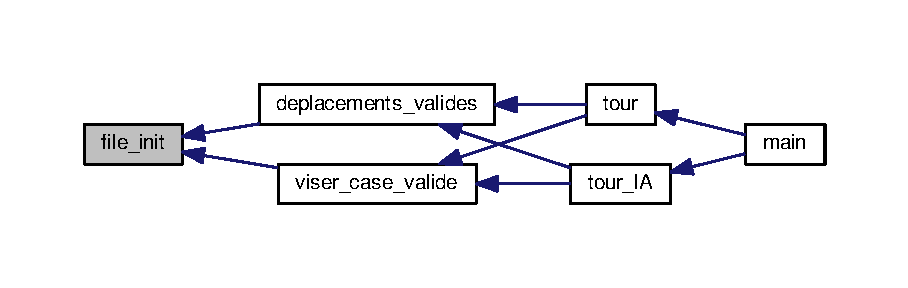
\includegraphics[width=350pt]{file_8c_a004123a6f8cce9d4168b0ea8cfdf133a_icgraph}
\end{center}
\end{figure}


\hypertarget{file_8c_a141d57004b90128d46274ba60f61249f}{\index{file.\-c@{file.\-c}!file\-\_\-liste\-\_\-afficher\-\_\-queue@{file\-\_\-liste\-\_\-afficher\-\_\-queue}}
\index{file\-\_\-liste\-\_\-afficher\-\_\-queue@{file\-\_\-liste\-\_\-afficher\-\_\-queue}!file.c@{file.\-c}}
\subsubsection[{file\-\_\-liste\-\_\-afficher\-\_\-queue}]{\setlength{\rightskip}{0pt plus 5cm}void file\-\_\-liste\-\_\-afficher\-\_\-queue (
\begin{DoxyParamCaption}
{}
\end{DoxyParamCaption}
)}}\label{file_8c_a141d57004b90128d46274ba60f61249f}


Définition à la ligne 47 du fichier file.\-c.

\hypertarget{file_8c_a59173755d515eb366fb01dba42a73e8e}{\index{file.\-c@{file.\-c}!file\-\_\-retirer@{file\-\_\-retirer}}
\index{file\-\_\-retirer@{file\-\_\-retirer}!file.c@{file.\-c}}
\subsubsection[{file\-\_\-retirer}]{\setlength{\rightskip}{0pt plus 5cm}void file\-\_\-retirer (
\begin{DoxyParamCaption}
\item[{{\bf t\-\_\-coord} $\ast$}]{val}
\end{DoxyParamCaption}
)}}\label{file_8c_a59173755d515eb366fb01dba42a73e8e}


Définition à la ligne 29 du fichier file.\-c.



Voici le graphe des appelants de cette fonction \-:\nopagebreak
\begin{figure}[H]
\begin{center}
\leavevmode
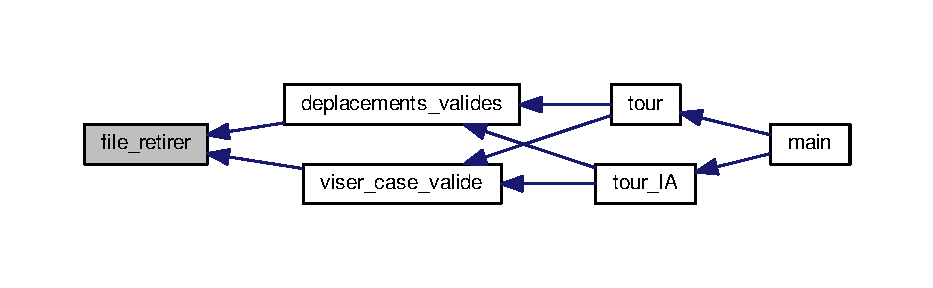
\includegraphics[width=350pt]{file_8c_a59173755d515eb366fb01dba42a73e8e_icgraph}
\end{center}
\end{figure}


\hypertarget{file_8c_a30c4f88a35783c4832434e9676ad98f5}{\index{file.\-c@{file.\-c}!file\-\_\-vide@{file\-\_\-vide}}
\index{file\-\_\-vide@{file\-\_\-vide}!file.c@{file.\-c}}
\subsubsection[{file\-\_\-vide}]{\setlength{\rightskip}{0pt plus 5cm}int file\-\_\-vide (
\begin{DoxyParamCaption}
{}
\end{DoxyParamCaption}
)}}\label{file_8c_a30c4f88a35783c4832434e9676ad98f5}


Définition à la ligne 42 du fichier file.\-c.


\hypertarget{file_8h}{\section{file.\-h File Reference}
\label{file_8h}\index{file.\-h@{file.\-h}}
}
{\ttfamily \#include \char`\"{}header.\-h\char`\"{}}\\*
Include dependency graph for file.\-h\-:
\nopagebreak
\begin{figure}[H]
\begin{center}
\leavevmode
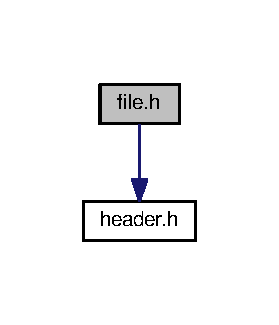
\includegraphics[width=134pt]{file_8h__incl}
\end{center}
\end{figure}
This graph shows which files directly or indirectly include this file\-:
\nopagebreak
\begin{figure}[H]
\begin{center}
\leavevmode
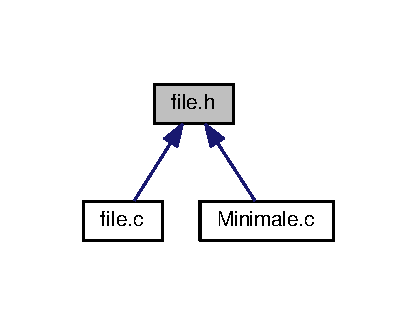
\includegraphics[width=200pt]{file_8h__dep__incl}
\end{center}
\end{figure}
\subsection*{Functions}
\begin{DoxyCompactItemize}
\item 
void \hyperlink{file_8h_a004123a6f8cce9d4168b0ea8cfdf133a}{file\-\_\-init} ()
\item 
void \hyperlink{file_8h_a9a4198b0c69187d42420b80f3e5b8d62}{file\-\_\-ajouter} (\hyperlink{structt__coord}{t\-\_\-coord} a)
\item 
void \hyperlink{file_8h_a59173755d515eb366fb01dba42a73e8e}{file\-\_\-retirer} (\hyperlink{structt__coord}{t\-\_\-coord} $\ast$val)
\item 
int \hyperlink{file_8h_a30c4f88a35783c4832434e9676ad98f5}{file\-\_\-vide} ()
\item 
void \hyperlink{file_8h_a141d57004b90128d46274ba60f61249f}{file\-\_\-liste\-\_\-afficher\-\_\-queue} ()
\item 
void \hyperlink{file_8h_a96c6e33606180f008c28906ff16f873a}{file\-\_\-afficher\-\_\-elt} (\hyperlink{structt__coord}{t\-\_\-coord} val)
\end{DoxyCompactItemize}


\subsection{Function Documentation}
\hypertarget{file_8h_a96c6e33606180f008c28906ff16f873a}{\index{file.\-h@{file.\-h}!file\-\_\-afficher\-\_\-elt@{file\-\_\-afficher\-\_\-elt}}
\index{file\-\_\-afficher\-\_\-elt@{file\-\_\-afficher\-\_\-elt}!file.h@{file.\-h}}
\subsubsection[{file\-\_\-afficher\-\_\-elt}]{\setlength{\rightskip}{0pt plus 5cm}void file\-\_\-afficher\-\_\-elt (
\begin{DoxyParamCaption}
\item[{{\bf t\-\_\-coord}}]{val}
\end{DoxyParamCaption}
)}}\label{file_8h_a96c6e33606180f008c28906ff16f873a}


Definition at line 53 of file file.\-c.

\hypertarget{file_8h_a9a4198b0c69187d42420b80f3e5b8d62}{\index{file.\-h@{file.\-h}!file\-\_\-ajouter@{file\-\_\-ajouter}}
\index{file\-\_\-ajouter@{file\-\_\-ajouter}!file.h@{file.\-h}}
\subsubsection[{file\-\_\-ajouter}]{\setlength{\rightskip}{0pt plus 5cm}void file\-\_\-ajouter (
\begin{DoxyParamCaption}
\item[{{\bf t\-\_\-coord}}]{a}
\end{DoxyParamCaption}
)}}\label{file_8h_a9a4198b0c69187d42420b80f3e5b8d62}


Definition at line 16 of file file.\-c.



Here is the caller graph for this function\-:
\nopagebreak
\begin{figure}[H]
\begin{center}
\leavevmode
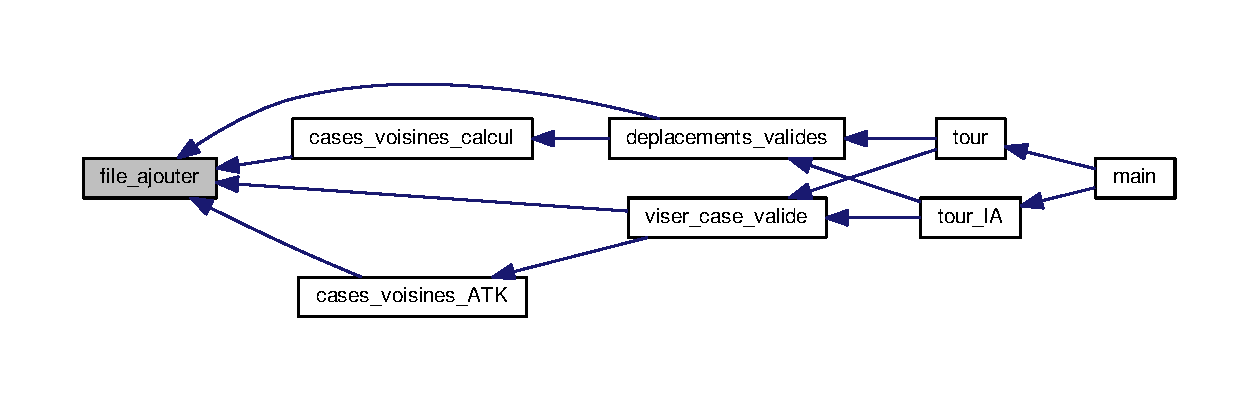
\includegraphics[width=350pt]{file_8h_a9a4198b0c69187d42420b80f3e5b8d62_icgraph}
\end{center}
\end{figure}


\hypertarget{file_8h_a004123a6f8cce9d4168b0ea8cfdf133a}{\index{file.\-h@{file.\-h}!file\-\_\-init@{file\-\_\-init}}
\index{file\-\_\-init@{file\-\_\-init}!file.h@{file.\-h}}
\subsubsection[{file\-\_\-init}]{\setlength{\rightskip}{0pt plus 5cm}void file\-\_\-init (
\begin{DoxyParamCaption}
{}
\end{DoxyParamCaption}
)}}\label{file_8h_a004123a6f8cce9d4168b0ea8cfdf133a}


Definition at line 8 of file file.\-c.



Here is the caller graph for this function\-:
\nopagebreak
\begin{figure}[H]
\begin{center}
\leavevmode
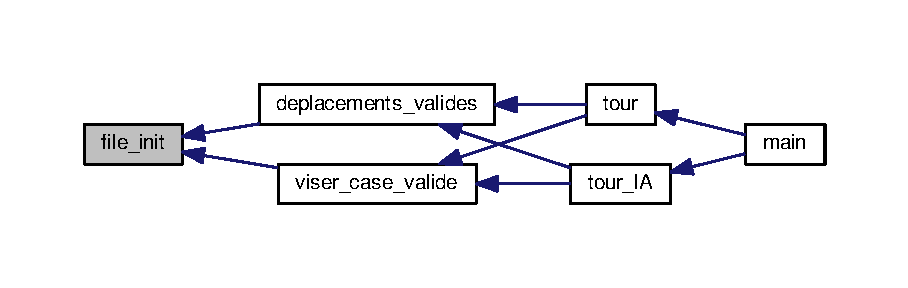
\includegraphics[width=350pt]{file_8h_a004123a6f8cce9d4168b0ea8cfdf133a_icgraph}
\end{center}
\end{figure}


\hypertarget{file_8h_a141d57004b90128d46274ba60f61249f}{\index{file.\-h@{file.\-h}!file\-\_\-liste\-\_\-afficher\-\_\-queue@{file\-\_\-liste\-\_\-afficher\-\_\-queue}}
\index{file\-\_\-liste\-\_\-afficher\-\_\-queue@{file\-\_\-liste\-\_\-afficher\-\_\-queue}!file.h@{file.\-h}}
\subsubsection[{file\-\_\-liste\-\_\-afficher\-\_\-queue}]{\setlength{\rightskip}{0pt plus 5cm}void file\-\_\-liste\-\_\-afficher\-\_\-queue (
\begin{DoxyParamCaption}
{}
\end{DoxyParamCaption}
)}}\label{file_8h_a141d57004b90128d46274ba60f61249f}


Definition at line 47 of file file.\-c.

\hypertarget{file_8h_a59173755d515eb366fb01dba42a73e8e}{\index{file.\-h@{file.\-h}!file\-\_\-retirer@{file\-\_\-retirer}}
\index{file\-\_\-retirer@{file\-\_\-retirer}!file.h@{file.\-h}}
\subsubsection[{file\-\_\-retirer}]{\setlength{\rightskip}{0pt plus 5cm}void file\-\_\-retirer (
\begin{DoxyParamCaption}
\item[{{\bf t\-\_\-coord} $\ast$}]{val}
\end{DoxyParamCaption}
)}}\label{file_8h_a59173755d515eb366fb01dba42a73e8e}


Definition at line 29 of file file.\-c.



Here is the caller graph for this function\-:
\nopagebreak
\begin{figure}[H]
\begin{center}
\leavevmode
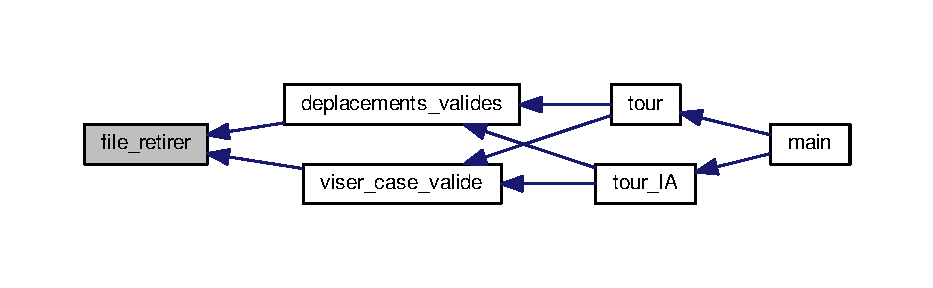
\includegraphics[width=350pt]{file_8h_a59173755d515eb366fb01dba42a73e8e_icgraph}
\end{center}
\end{figure}


\hypertarget{file_8h_a30c4f88a35783c4832434e9676ad98f5}{\index{file.\-h@{file.\-h}!file\-\_\-vide@{file\-\_\-vide}}
\index{file\-\_\-vide@{file\-\_\-vide}!file.h@{file.\-h}}
\subsubsection[{file\-\_\-vide}]{\setlength{\rightskip}{0pt plus 5cm}int file\-\_\-vide (
\begin{DoxyParamCaption}
{}
\end{DoxyParamCaption}
)}}\label{file_8h_a30c4f88a35783c4832434e9676ad98f5}


Definition at line 42 of file file.\-c.


\hypertarget{header_8h}{\section{Référence du fichier header.\-h}
\label{header_8h}\index{header.\-h@{header.\-h}}
}
Ce graphe montre quels fichiers incluent directement ou indirectement ce fichier \-:
\nopagebreak
\begin{figure}[H]
\begin{center}
\leavevmode
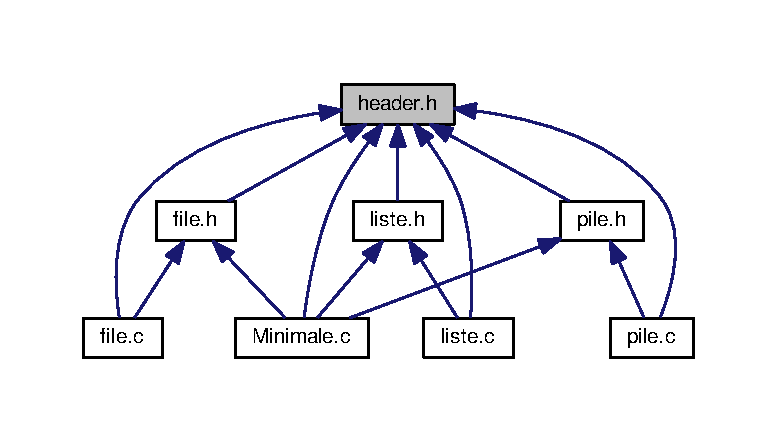
\includegraphics[width=350pt]{header_8h__dep__incl}
\end{center}
\end{figure}
\subsection*{Structures de données}
\begin{DoxyCompactItemize}
\item 
struct \hyperlink{structt__status}{t\-\_\-status}
\item 
struct \hyperlink{structt__stats}{t\-\_\-stats}
\item 
struct \hyperlink{structt__coord}{t\-\_\-coord}
\item 
struct \hyperlink{structt__skill}{t\-\_\-skill}
\item 
struct \hyperlink{structt__skill__list}{t\-\_\-skill\-\_\-list}
\item 
struct \hyperlink{structt__character}{t\-\_\-character}
\item 
struct \hyperlink{structt__player}{t\-\_\-player}
\end{DoxyCompactItemize}
\subsection*{Macros}
\begin{DoxyCompactItemize}
\item 
\#define \hyperlink{header_8h_a523c276fa2df3dd24764b5bb500dbde6}{T\-A\-I\-L\-L\-E\-\_\-\-M\-A\-T\-R\-I\-C\-E}~5
\item 
\#define \hyperlink{header_8h_a220380eaa4bfe0ffeab9859c6f3d2076}{Max\-Tab}~40
\item 
\#define \hyperlink{header_8h_ab154998a3a376095f3601bc35c5cf523}{Max\-String}~40
\item 
\#define \hyperlink{header_8h_abcbf07dd09e51c934ff60872f465727a}{bloc1}~((char)178)
\item 
\#define \hyperlink{header_8h_a6f35bce5de1d159bff01cc3d33c9c72c}{bloc2}~((char)219)
\item 
\#define \hyperlink{header_8h_a54589dbd40ede83ce0d307134bed6999}{bloc3}~((char)254)
\item 
\#define \hyperlink{header_8h_a293f382892dd9160685d3131e4881495}{skill\-\_\-attack}~((\hyperlink{structt__skill}{t\-\_\-skill})\{\char`\"{}Coup\char`\"{},1,A\-T\-K,1\})
\item 
\#define \hyperlink{header_8h_ae6f347a0b1e26425b82734df3904273d}{skill\-\_\-empty}~((\hyperlink{structt__skill}{t\-\_\-skill})\{\char`\"{}\char`\"{},0,\hyperlink{header_8h_a440f669d36bc2028077af38574051204a2f0d18fc0d0fa4a6cd92dc328501874d}{E\-M\-P\-T\-Y},0\})
\item 
\#define \hyperlink{header_8h_ae423278c3d83b22e7ba58f31c1d4722a}{skill\-\_\-skip}~((\hyperlink{structt__skill}{t\-\_\-skill})\{\char`\"{}Passer le \hyperlink{_minimale_8c_a779ee1563d913e90d9ad93b9adf6867e}{tour}\char`\"{},0,E\-M\-P\-T\-Y,0\})
\item 
\#define \hyperlink{header_8h_a6cbdba3415482afa3d3e831cd1a739a2}{coord\-\_\-default}~((\hyperlink{structt__coord}{t\-\_\-coord})\{-\/1,-\/1\})
\item 
\#define \hyperlink{header_8h_a5c4cefe49779a0cc311243c1bb97b120}{orientation\-\_\-default}~(\hyperlink{header_8h_a6dc6eccccaf78ef029cff998c0e654f4aebc281bf093563220c2270ba57dedfce}{up})
\item 
\#define \hyperlink{header_8h_a7c38568d47211679c8483fc60e185651}{status\-\_\-default}~((\hyperlink{structt__status}{t\-\_\-status})\{30,30,10,10\})
\item 
\#define \hyperlink{header_8h_ad92274bc74ce5fee209d6177f46b06e3}{status\-\_\-\-\_\-terrain\-\_\-default}~((\hyperlink{structt__status}{t\-\_\-status})\{0,0,0,0\})
\item 
\#define \hyperlink{header_8h_af720a86d25a368a1484318d8a877961b}{stats\-\_\-default}~((\hyperlink{structt__stats}{t\-\_\-stats})\{10,10,10,10,2\})
\item 
\#define \hyperlink{header_8h_a06744a7db35a5caffebfeef65fecff32}{stats\-\_\-terrain\-\_\-default}~((\hyperlink{structt__stats}{t\-\_\-stats})\{0,0,0,0,0\})
\item 
\#define \hyperlink{header_8h_a661f2fa1a0f9707f5a19494debc26d68}{skill\-\_\-list\-\_\-default}~((\hyperlink{structt__skill__list}{t\-\_\-skill\-\_\-list})\{ \hyperlink{header_8h_a293f382892dd9160685d3131e4881495}{skill\-\_\-attack},\hyperlink{header_8h_ae6f347a0b1e26425b82734df3904273d}{skill\-\_\-empty},\hyperlink{header_8h_ae6f347a0b1e26425b82734df3904273d}{skill\-\_\-empty},\hyperlink{header_8h_ae6f347a0b1e26425b82734df3904273d}{skill\-\_\-empty},\hyperlink{header_8h_ae6f347a0b1e26425b82734df3904273d}{skill\-\_\-empty},\hyperlink{header_8h_ae423278c3d83b22e7ba58f31c1d4722a}{skill\-\_\-skip}\})
\item 
\#define \hyperlink{header_8h_ae31f7588359442249a6f01914a7eb769}{empty\-\_\-skill\-\_\-list}~((\hyperlink{structt__skill__list}{t\-\_\-skill\-\_\-list})\{\hyperlink{header_8h_ae6f347a0b1e26425b82734df3904273d}{skill\-\_\-empty},\hyperlink{header_8h_ae6f347a0b1e26425b82734df3904273d}{skill\-\_\-empty},\hyperlink{header_8h_ae6f347a0b1e26425b82734df3904273d}{skill\-\_\-empty},\hyperlink{header_8h_ae6f347a0b1e26425b82734df3904273d}{skill\-\_\-empty},\hyperlink{header_8h_ae6f347a0b1e26425b82734df3904273d}{skill\-\_\-empty},\hyperlink{header_8h_ae6f347a0b1e26425b82734df3904273d}{skill\-\_\-empty}\})
\item 
\#define \hyperlink{header_8h_a6e8b24c0508661b7539c8b9e38975508}{character\-\_\-default}~((\hyperlink{structt__character}{t\-\_\-character})\{\char`\"{}Default name\char`\"{}, coord\-\_\-default, \hyperlink{header_8h_a5c4cefe49779a0cc311243c1bb97b120}{orientation\-\_\-default}, \hyperlink{header_8h_a7c38568d47211679c8483fc60e185651}{status\-\_\-default}, \hyperlink{header_8h_af720a86d25a368a1484318d8a877961b}{stats\-\_\-default}, \hyperlink{header_8h_a661f2fa1a0f9707f5a19494debc26d68}{skill\-\_\-list\-\_\-default}, \hyperlink{header_8h_a4bb25c9352f7bb2ea2eb663ccf579528a4a0e079df1b0c47b395b996f7240b48c}{sauvage}, 1\})
\item 
\#define \hyperlink{header_8h_ad8e55599d4e25ea791fd084a348e0967}{default\-\_\-target\-Orientation}~((\hyperlink{header_8h_a05b909310980a637d41bd67fc4d5c389}{t\-\_\-target\-Orientation})\hyperlink{header_8h_a05b909310980a637d41bd67fc4d5c389ab30562d2871f1a5b7d220569f54ccceb}{front})
\item 
\#define \hyperlink{header_8h_a05114c8c78053bf80235674b9d7440c4}{default\-\_\-trap}~((\hyperlink{structt__character}{t\-\_\-character})\{\char`\"{}Trap\char`\"{}, coord\-\_\-default, \hyperlink{header_8h_a5c4cefe49779a0cc311243c1bb97b120}{orientation\-\_\-default}, \hyperlink{header_8h_a7c38568d47211679c8483fc60e185651}{status\-\_\-default}, \hyperlink{header_8h_af720a86d25a368a1484318d8a877961b}{stats\-\_\-default}, \hyperlink{header_8h_a661f2fa1a0f9707f5a19494debc26d68}{skill\-\_\-list\-\_\-default}, 1, 1\})
\item 
\#define \hyperlink{header_8h_ab61d48d4ed3100c6e826da441b31cdbd}{curseur}~(char)254
\item 
\#define \hyperlink{header_8h_a7dd5f83f4f2f4ea483fc49807ff9f43b}{case\-\_\-terrain}~((\hyperlink{structt__character}{t\-\_\-character})\{\char`\"{}\char`\"{},\hyperlink{header_8h_a6cbdba3415482afa3d3e831cd1a739a2}{coord\-\_\-default} ,\hyperlink{header_8h_a5c4cefe49779a0cc311243c1bb97b120}{orientation\-\_\-default} ,\hyperlink{header_8h_ad92274bc74ce5fee209d6177f46b06e3}{status\-\_\-\-\_\-terrain\-\_\-default} ,\hyperlink{header_8h_a06744a7db35a5caffebfeef65fecff32}{stats\-\_\-terrain\-\_\-default} ,\hyperlink{header_8h_ae31f7588359442249a6f01914a7eb769}{empty\-\_\-skill\-\_\-list}, 0 , 0 \})
\item 
\#define \hyperlink{header_8h_a8a976ee03aa89e3b22be5595252d3c04}{case\-\_\-obstacle}~((\hyperlink{structt__character}{t\-\_\-character})\{\char`\"{}\char`\"{},\hyperlink{header_8h_a6cbdba3415482afa3d3e831cd1a739a2}{coord\-\_\-default} ,\hyperlink{header_8h_a5c4cefe49779a0cc311243c1bb97b120}{orientation\-\_\-default} ,\hyperlink{header_8h_a7c38568d47211679c8483fc60e185651}{status\-\_\-default} ,\hyperlink{header_8h_af720a86d25a368a1484318d8a877961b}{stats\-\_\-default} ,\hyperlink{header_8h_ae31f7588359442249a6f01914a7eb769}{empty\-\_\-skill\-\_\-list}, -\/1 , 0 \})
\end{DoxyCompactItemize}
\subsection*{Énumérations}
\begin{DoxyCompactItemize}
\item 
enum \hyperlink{header_8h_a4bb25c9352f7bb2ea2eb663ccf579528}{t\-\_\-camp} \{ \hyperlink{header_8h_a4bb25c9352f7bb2ea2eb663ccf579528a8703eca1f6f779dd8bebfc200139b07d}{obstacle} =-\/1, 
\hyperlink{header_8h_a4bb25c9352f7bb2ea2eb663ccf579528ae55222d4b0e83581c51f843e87e3cfe2}{terrain} =0, 
\hyperlink{header_8h_a4bb25c9352f7bb2ea2eb663ccf579528a4a0e079df1b0c47b395b996f7240b48c}{sauvage} =1
 \}
\item 
enum \hyperlink{header_8h_a440f669d36bc2028077af38574051204}{t\-\_\-skilltype} \{ \hyperlink{header_8h_a440f669d36bc2028077af38574051204a2f0d18fc0d0fa4a6cd92dc328501874d}{E\-M\-P\-T\-Y}, 
\hyperlink{header_8h_a440f669d36bc2028077af38574051204a52c6d49f971f8f70cf3f3c474edc08f9}{A\-T\-K}, 
\hyperlink{header_8h_a440f669d36bc2028077af38574051204a1fe261f2a80ef9b7055433a3c2d93af8}{M\-A\-T\-K}, 
\hyperlink{header_8h_a440f669d36bc2028077af38574051204ac0533b6cb94383273589b6764c8a0796}{T\-R\-A\-P}
 \}
\item 
enum \hyperlink{header_8h_a6dc6eccccaf78ef029cff998c0e654f4}{t\-\_\-orientation} \{ \hyperlink{header_8h_a6dc6eccccaf78ef029cff998c0e654f4aebc281bf093563220c2270ba57dedfce}{up}, 
\hyperlink{header_8h_a6dc6eccccaf78ef029cff998c0e654f4af763d610923b0c4614e8ecd65212666a}{right}, 
\hyperlink{header_8h_a6dc6eccccaf78ef029cff998c0e654f4a00156fc42b17a87d0746d97b42caf296}{down}, 
\hyperlink{header_8h_a6dc6eccccaf78ef029cff998c0e654f4ab0ac36b187aa60c167ffcead3d5a03c0}{left}
 \}
\item 
enum \hyperlink{header_8h_a05b909310980a637d41bd67fc4d5c389}{t\-\_\-target\-Orientation} \{ \hyperlink{header_8h_a05b909310980a637d41bd67fc4d5c389ab30562d2871f1a5b7d220569f54ccceb}{front}, 
\hyperlink{header_8h_a05b909310980a637d41bd67fc4d5c389a6e20889cbd4a669c96acec7eb0f836f4}{side}, 
\hyperlink{header_8h_a05b909310980a637d41bd67fc4d5c389aa0cf137e48905c39b94f23a05b14e7c9}{back}
 \}
\item 
enum \hyperlink{header_8h_ac8020d257c824e4b188c04ee386ebfda}{t\-\_\-character\-\_\-type} \{ \hyperlink{header_8h_ac8020d257c824e4b188c04ee386ebfdaa88bc03071d883ba67f80a4dbc8712ab5}{L\-A\-N\-D\-\_\-\-U\-N\-I\-T}, 
\hyperlink{header_8h_ac8020d257c824e4b188c04ee386ebfdaad28f3d40a0201f066f5b8adb539a5a94}{A\-I\-R\-\_\-\-U\-N\-I\-T}, 
\hyperlink{header_8h_ac8020d257c824e4b188c04ee386ebfdaa6d5cb476c95a2f13156fa5d298afa208}{J\-U\-M\-P\-I\-N\-G\-\_\-\-U\-N\-I\-T}, 
\hyperlink{header_8h_ac8020d257c824e4b188c04ee386ebfdaa5b5e1b4421db434bf27a112d197081e1}{T\-R\-A\-P\-\_\-\-U\-N\-I\-T}
 \}
\end{DoxyCompactItemize}


\subsection{Documentation des macros}
\hypertarget{header_8h_abcbf07dd09e51c934ff60872f465727a}{\index{header.\-h@{header.\-h}!bloc1@{bloc1}}
\index{bloc1@{bloc1}!header.h@{header.\-h}}
\subsubsection[{bloc1}]{\setlength{\rightskip}{0pt plus 5cm}\#define bloc1~((char)178)}}\label{header_8h_abcbf07dd09e51c934ff60872f465727a}


Définition à la ligne 8 du fichier header.\-h.

\hypertarget{header_8h_a6f35bce5de1d159bff01cc3d33c9c72c}{\index{header.\-h@{header.\-h}!bloc2@{bloc2}}
\index{bloc2@{bloc2}!header.h@{header.\-h}}
\subsubsection[{bloc2}]{\setlength{\rightskip}{0pt plus 5cm}\#define bloc2~((char)219)}}\label{header_8h_a6f35bce5de1d159bff01cc3d33c9c72c}


Définition à la ligne 9 du fichier header.\-h.

\hypertarget{header_8h_a54589dbd40ede83ce0d307134bed6999}{\index{header.\-h@{header.\-h}!bloc3@{bloc3}}
\index{bloc3@{bloc3}!header.h@{header.\-h}}
\subsubsection[{bloc3}]{\setlength{\rightskip}{0pt plus 5cm}\#define bloc3~((char)254)}}\label{header_8h_a54589dbd40ede83ce0d307134bed6999}


Définition à la ligne 10 du fichier header.\-h.

\hypertarget{header_8h_a8a976ee03aa89e3b22be5595252d3c04}{\index{header.\-h@{header.\-h}!case\-\_\-obstacle@{case\-\_\-obstacle}}
\index{case\-\_\-obstacle@{case\-\_\-obstacle}!header.h@{header.\-h}}
\subsubsection[{case\-\_\-obstacle}]{\setlength{\rightskip}{0pt plus 5cm}\#define case\-\_\-obstacle~(({\bf t\-\_\-character})\{\char`\"{}\char`\"{},{\bf coord\-\_\-default} ,{\bf orientation\-\_\-default} ,{\bf status\-\_\-default} ,{\bf stats\-\_\-default} ,{\bf empty\-\_\-skill\-\_\-list}, -\/1 , 0 \})}}\label{header_8h_a8a976ee03aa89e3b22be5595252d3c04}


Définition à la ligne 30 du fichier header.\-h.

\hypertarget{header_8h_a7dd5f83f4f2f4ea483fc49807ff9f43b}{\index{header.\-h@{header.\-h}!case\-\_\-terrain@{case\-\_\-terrain}}
\index{case\-\_\-terrain@{case\-\_\-terrain}!header.h@{header.\-h}}
\subsubsection[{case\-\_\-terrain}]{\setlength{\rightskip}{0pt plus 5cm}\#define case\-\_\-terrain~(({\bf t\-\_\-character})\{\char`\"{}\char`\"{},{\bf coord\-\_\-default} ,{\bf orientation\-\_\-default} ,{\bf status\-\_\-\-\_\-terrain\-\_\-default} ,{\bf stats\-\_\-terrain\-\_\-default} ,{\bf empty\-\_\-skill\-\_\-list}, 0 , 0 \})}}\label{header_8h_a7dd5f83f4f2f4ea483fc49807ff9f43b}


Définition à la ligne 29 du fichier header.\-h.

\hypertarget{header_8h_a6e8b24c0508661b7539c8b9e38975508}{\index{header.\-h@{header.\-h}!character\-\_\-default@{character\-\_\-default}}
\index{character\-\_\-default@{character\-\_\-default}!header.h@{header.\-h}}
\subsubsection[{character\-\_\-default}]{\setlength{\rightskip}{0pt plus 5cm}\#define character\-\_\-default~(({\bf t\-\_\-character})\{\char`\"{}Default name\char`\"{}, coord\-\_\-default, {\bf orientation\-\_\-default}, {\bf status\-\_\-default}, {\bf stats\-\_\-default}, {\bf skill\-\_\-list\-\_\-default}, {\bf sauvage}, 1\})}}\label{header_8h_a6e8b24c0508661b7539c8b9e38975508}


Définition à la ligne 23 du fichier header.\-h.

\hypertarget{header_8h_a6cbdba3415482afa3d3e831cd1a739a2}{\index{header.\-h@{header.\-h}!coord\-\_\-default@{coord\-\_\-default}}
\index{coord\-\_\-default@{coord\-\_\-default}!header.h@{header.\-h}}
\subsubsection[{coord\-\_\-default}]{\setlength{\rightskip}{0pt plus 5cm}\#define coord\-\_\-default~(({\bf t\-\_\-coord})\{-\/1,-\/1\})}}\label{header_8h_a6cbdba3415482afa3d3e831cd1a739a2}


Définition à la ligne 15 du fichier header.\-h.

\hypertarget{header_8h_ab61d48d4ed3100c6e826da441b31cdbd}{\index{header.\-h@{header.\-h}!curseur@{curseur}}
\index{curseur@{curseur}!header.h@{header.\-h}}
\subsubsection[{curseur}]{\setlength{\rightskip}{0pt plus 5cm}\#define curseur~(char)254}}\label{header_8h_ab61d48d4ed3100c6e826da441b31cdbd}


Définition à la ligne 27 du fichier header.\-h.

\hypertarget{header_8h_ad8e55599d4e25ea791fd084a348e0967}{\index{header.\-h@{header.\-h}!default\-\_\-target\-Orientation@{default\-\_\-target\-Orientation}}
\index{default\-\_\-target\-Orientation@{default\-\_\-target\-Orientation}!header.h@{header.\-h}}
\subsubsection[{default\-\_\-target\-Orientation}]{\setlength{\rightskip}{0pt plus 5cm}\#define default\-\_\-target\-Orientation~(({\bf t\-\_\-target\-Orientation}){\bf front})}}\label{header_8h_ad8e55599d4e25ea791fd084a348e0967}


Définition à la ligne 24 du fichier header.\-h.

\hypertarget{header_8h_a05114c8c78053bf80235674b9d7440c4}{\index{header.\-h@{header.\-h}!default\-\_\-trap@{default\-\_\-trap}}
\index{default\-\_\-trap@{default\-\_\-trap}!header.h@{header.\-h}}
\subsubsection[{default\-\_\-trap}]{\setlength{\rightskip}{0pt plus 5cm}\#define default\-\_\-trap~(({\bf t\-\_\-character})\{\char`\"{}Trap\char`\"{}, coord\-\_\-default, {\bf orientation\-\_\-default}, {\bf status\-\_\-default}, {\bf stats\-\_\-default}, {\bf skill\-\_\-list\-\_\-default}, 1, 1\})}}\label{header_8h_a05114c8c78053bf80235674b9d7440c4}


Définition à la ligne 25 du fichier header.\-h.

\hypertarget{header_8h_ae31f7588359442249a6f01914a7eb769}{\index{header.\-h@{header.\-h}!empty\-\_\-skill\-\_\-list@{empty\-\_\-skill\-\_\-list}}
\index{empty\-\_\-skill\-\_\-list@{empty\-\_\-skill\-\_\-list}!header.h@{header.\-h}}
\subsubsection[{empty\-\_\-skill\-\_\-list}]{\setlength{\rightskip}{0pt plus 5cm}\#define empty\-\_\-skill\-\_\-list~(({\bf t\-\_\-skill\-\_\-list})\{{\bf skill\-\_\-empty},{\bf skill\-\_\-empty},{\bf skill\-\_\-empty},{\bf skill\-\_\-empty},{\bf skill\-\_\-empty},{\bf skill\-\_\-empty}\})}}\label{header_8h_ae31f7588359442249a6f01914a7eb769}


Définition à la ligne 22 du fichier header.\-h.

\hypertarget{header_8h_ab154998a3a376095f3601bc35c5cf523}{\index{header.\-h@{header.\-h}!Max\-String@{Max\-String}}
\index{Max\-String@{Max\-String}!header.h@{header.\-h}}
\subsubsection[{Max\-String}]{\setlength{\rightskip}{0pt plus 5cm}\#define Max\-String~40}}\label{header_8h_ab154998a3a376095f3601bc35c5cf523}


Définition à la ligne 6 du fichier header.\-h.

\hypertarget{header_8h_a220380eaa4bfe0ffeab9859c6f3d2076}{\index{header.\-h@{header.\-h}!Max\-Tab@{Max\-Tab}}
\index{Max\-Tab@{Max\-Tab}!header.h@{header.\-h}}
\subsubsection[{Max\-Tab}]{\setlength{\rightskip}{0pt plus 5cm}\#define Max\-Tab~40}}\label{header_8h_a220380eaa4bfe0ffeab9859c6f3d2076}


Définition à la ligne 5 du fichier header.\-h.

\hypertarget{header_8h_a5c4cefe49779a0cc311243c1bb97b120}{\index{header.\-h@{header.\-h}!orientation\-\_\-default@{orientation\-\_\-default}}
\index{orientation\-\_\-default@{orientation\-\_\-default}!header.h@{header.\-h}}
\subsubsection[{orientation\-\_\-default}]{\setlength{\rightskip}{0pt plus 5cm}\#define orientation\-\_\-default~({\bf up})}}\label{header_8h_a5c4cefe49779a0cc311243c1bb97b120}


Définition à la ligne 16 du fichier header.\-h.

\hypertarget{header_8h_a293f382892dd9160685d3131e4881495}{\index{header.\-h@{header.\-h}!skill\-\_\-attack@{skill\-\_\-attack}}
\index{skill\-\_\-attack@{skill\-\_\-attack}!header.h@{header.\-h}}
\subsubsection[{skill\-\_\-attack}]{\setlength{\rightskip}{0pt plus 5cm}\#define skill\-\_\-attack~(({\bf t\-\_\-skill})\{\char`\"{}Coup\char`\"{},1,A\-T\-K,1\})}}\label{header_8h_a293f382892dd9160685d3131e4881495}


Définition à la ligne 12 du fichier header.\-h.

\hypertarget{header_8h_ae6f347a0b1e26425b82734df3904273d}{\index{header.\-h@{header.\-h}!skill\-\_\-empty@{skill\-\_\-empty}}
\index{skill\-\_\-empty@{skill\-\_\-empty}!header.h@{header.\-h}}
\subsubsection[{skill\-\_\-empty}]{\setlength{\rightskip}{0pt plus 5cm}\#define skill\-\_\-empty~(({\bf t\-\_\-skill})\{\char`\"{}\char`\"{},0,{\bf E\-M\-P\-T\-Y},0\})}}\label{header_8h_ae6f347a0b1e26425b82734df3904273d}


Définition à la ligne 13 du fichier header.\-h.

\hypertarget{header_8h_a661f2fa1a0f9707f5a19494debc26d68}{\index{header.\-h@{header.\-h}!skill\-\_\-list\-\_\-default@{skill\-\_\-list\-\_\-default}}
\index{skill\-\_\-list\-\_\-default@{skill\-\_\-list\-\_\-default}!header.h@{header.\-h}}
\subsubsection[{skill\-\_\-list\-\_\-default}]{\setlength{\rightskip}{0pt plus 5cm}\#define skill\-\_\-list\-\_\-default~(({\bf t\-\_\-skill\-\_\-list})\{ {\bf skill\-\_\-attack},{\bf skill\-\_\-empty},{\bf skill\-\_\-empty},{\bf skill\-\_\-empty},{\bf skill\-\_\-empty},{\bf skill\-\_\-skip}\})}}\label{header_8h_a661f2fa1a0f9707f5a19494debc26d68}


Définition à la ligne 21 du fichier header.\-h.

\hypertarget{header_8h_ae423278c3d83b22e7ba58f31c1d4722a}{\index{header.\-h@{header.\-h}!skill\-\_\-skip@{skill\-\_\-skip}}
\index{skill\-\_\-skip@{skill\-\_\-skip}!header.h@{header.\-h}}
\subsubsection[{skill\-\_\-skip}]{\setlength{\rightskip}{0pt plus 5cm}\#define skill\-\_\-skip~(({\bf t\-\_\-skill})\{\char`\"{}Passer le {\bf tour}\char`\"{},0,E\-M\-P\-T\-Y,0\})}}\label{header_8h_ae423278c3d83b22e7ba58f31c1d4722a}


Définition à la ligne 14 du fichier header.\-h.

\hypertarget{header_8h_af720a86d25a368a1484318d8a877961b}{\index{header.\-h@{header.\-h}!stats\-\_\-default@{stats\-\_\-default}}
\index{stats\-\_\-default@{stats\-\_\-default}!header.h@{header.\-h}}
\subsubsection[{stats\-\_\-default}]{\setlength{\rightskip}{0pt plus 5cm}\#define stats\-\_\-default~(({\bf t\-\_\-stats})\{10,10,10,10,2\})}}\label{header_8h_af720a86d25a368a1484318d8a877961b}


Définition à la ligne 19 du fichier header.\-h.

\hypertarget{header_8h_a06744a7db35a5caffebfeef65fecff32}{\index{header.\-h@{header.\-h}!stats\-\_\-terrain\-\_\-default@{stats\-\_\-terrain\-\_\-default}}
\index{stats\-\_\-terrain\-\_\-default@{stats\-\_\-terrain\-\_\-default}!header.h@{header.\-h}}
\subsubsection[{stats\-\_\-terrain\-\_\-default}]{\setlength{\rightskip}{0pt plus 5cm}\#define stats\-\_\-terrain\-\_\-default~(({\bf t\-\_\-stats})\{0,0,0,0,0\})}}\label{header_8h_a06744a7db35a5caffebfeef65fecff32}


Définition à la ligne 20 du fichier header.\-h.

\hypertarget{header_8h_ad92274bc74ce5fee209d6177f46b06e3}{\index{header.\-h@{header.\-h}!status\-\_\-\-\_\-terrain\-\_\-default@{status\-\_\-\-\_\-terrain\-\_\-default}}
\index{status\-\_\-\-\_\-terrain\-\_\-default@{status\-\_\-\-\_\-terrain\-\_\-default}!header.h@{header.\-h}}
\subsubsection[{status\-\_\-\-\_\-terrain\-\_\-default}]{\setlength{\rightskip}{0pt plus 5cm}\#define status\-\_\-\-\_\-terrain\-\_\-default~(({\bf t\-\_\-status})\{0,0,0,0\})}}\label{header_8h_ad92274bc74ce5fee209d6177f46b06e3}


Définition à la ligne 18 du fichier header.\-h.

\hypertarget{header_8h_a7c38568d47211679c8483fc60e185651}{\index{header.\-h@{header.\-h}!status\-\_\-default@{status\-\_\-default}}
\index{status\-\_\-default@{status\-\_\-default}!header.h@{header.\-h}}
\subsubsection[{status\-\_\-default}]{\setlength{\rightskip}{0pt plus 5cm}\#define status\-\_\-default~(({\bf t\-\_\-status})\{30,30,10,10\})}}\label{header_8h_a7c38568d47211679c8483fc60e185651}


Définition à la ligne 17 du fichier header.\-h.

\hypertarget{header_8h_a523c276fa2df3dd24764b5bb500dbde6}{\index{header.\-h@{header.\-h}!T\-A\-I\-L\-L\-E\-\_\-\-M\-A\-T\-R\-I\-C\-E@{T\-A\-I\-L\-L\-E\-\_\-\-M\-A\-T\-R\-I\-C\-E}}
\index{T\-A\-I\-L\-L\-E\-\_\-\-M\-A\-T\-R\-I\-C\-E@{T\-A\-I\-L\-L\-E\-\_\-\-M\-A\-T\-R\-I\-C\-E}!header.h@{header.\-h}}
\subsubsection[{T\-A\-I\-L\-L\-E\-\_\-\-M\-A\-T\-R\-I\-C\-E}]{\setlength{\rightskip}{0pt plus 5cm}\#define T\-A\-I\-L\-L\-E\-\_\-\-M\-A\-T\-R\-I\-C\-E~5}}\label{header_8h_a523c276fa2df3dd24764b5bb500dbde6}


Définition à la ligne 4 du fichier header.\-h.



\subsection{Documentation du type de l'énumération}
\hypertarget{header_8h_a4bb25c9352f7bb2ea2eb663ccf579528}{\index{header.\-h@{header.\-h}!t\-\_\-camp@{t\-\_\-camp}}
\index{t\-\_\-camp@{t\-\_\-camp}!header.h@{header.\-h}}
\subsubsection[{t\-\_\-camp}]{\setlength{\rightskip}{0pt plus 5cm}enum {\bf t\-\_\-camp}}}\label{header_8h_a4bb25c9352f7bb2ea2eb663ccf579528}
\begin{Desc}
\item[Valeurs énumérées]\par
\begin{description}
\index{obstacle@{obstacle}!header.\-h@{header.\-h}}\index{header.\-h@{header.\-h}!obstacle@{obstacle}}\item[{\em 
\hypertarget{header_8h_a4bb25c9352f7bb2ea2eb663ccf579528a8703eca1f6f779dd8bebfc200139b07d}{obstacle}\label{header_8h_a4bb25c9352f7bb2ea2eb663ccf579528a8703eca1f6f779dd8bebfc200139b07d}
}]\index{terrain@{terrain}!header.\-h@{header.\-h}}\index{header.\-h@{header.\-h}!terrain@{terrain}}\item[{\em 
\hypertarget{header_8h_a4bb25c9352f7bb2ea2eb663ccf579528ae55222d4b0e83581c51f843e87e3cfe2}{terrain}\label{header_8h_a4bb25c9352f7bb2ea2eb663ccf579528ae55222d4b0e83581c51f843e87e3cfe2}
}]\index{sauvage@{sauvage}!header.\-h@{header.\-h}}\index{header.\-h@{header.\-h}!sauvage@{sauvage}}\item[{\em 
\hypertarget{header_8h_a4bb25c9352f7bb2ea2eb663ccf579528a4a0e079df1b0c47b395b996f7240b48c}{sauvage}\label{header_8h_a4bb25c9352f7bb2ea2eb663ccf579528a4a0e079df1b0c47b395b996f7240b48c}
}]\end{description}
\end{Desc}


Définition à la ligne 32 du fichier header.\-h.

\hypertarget{header_8h_ac8020d257c824e4b188c04ee386ebfda}{\index{header.\-h@{header.\-h}!t\-\_\-character\-\_\-type@{t\-\_\-character\-\_\-type}}
\index{t\-\_\-character\-\_\-type@{t\-\_\-character\-\_\-type}!header.h@{header.\-h}}
\subsubsection[{t\-\_\-character\-\_\-type}]{\setlength{\rightskip}{0pt plus 5cm}enum {\bf t\-\_\-character\-\_\-type}}}\label{header_8h_ac8020d257c824e4b188c04ee386ebfda}
\begin{Desc}
\item[Valeurs énumérées]\par
\begin{description}
\index{L\-A\-N\-D\-\_\-\-U\-N\-I\-T@{L\-A\-N\-D\-\_\-\-U\-N\-I\-T}!header.\-h@{header.\-h}}\index{header.\-h@{header.\-h}!L\-A\-N\-D\-\_\-\-U\-N\-I\-T@{L\-A\-N\-D\-\_\-\-U\-N\-I\-T}}\item[{\em 
\hypertarget{header_8h_ac8020d257c824e4b188c04ee386ebfdaa88bc03071d883ba67f80a4dbc8712ab5}{L\-A\-N\-D\-\_\-\-U\-N\-I\-T}\label{header_8h_ac8020d257c824e4b188c04ee386ebfdaa88bc03071d883ba67f80a4dbc8712ab5}
}]\index{A\-I\-R\-\_\-\-U\-N\-I\-T@{A\-I\-R\-\_\-\-U\-N\-I\-T}!header.\-h@{header.\-h}}\index{header.\-h@{header.\-h}!A\-I\-R\-\_\-\-U\-N\-I\-T@{A\-I\-R\-\_\-\-U\-N\-I\-T}}\item[{\em 
\hypertarget{header_8h_ac8020d257c824e4b188c04ee386ebfdaad28f3d40a0201f066f5b8adb539a5a94}{A\-I\-R\-\_\-\-U\-N\-I\-T}\label{header_8h_ac8020d257c824e4b188c04ee386ebfdaad28f3d40a0201f066f5b8adb539a5a94}
}]\index{J\-U\-M\-P\-I\-N\-G\-\_\-\-U\-N\-I\-T@{J\-U\-M\-P\-I\-N\-G\-\_\-\-U\-N\-I\-T}!header.\-h@{header.\-h}}\index{header.\-h@{header.\-h}!J\-U\-M\-P\-I\-N\-G\-\_\-\-U\-N\-I\-T@{J\-U\-M\-P\-I\-N\-G\-\_\-\-U\-N\-I\-T}}\item[{\em 
\hypertarget{header_8h_ac8020d257c824e4b188c04ee386ebfdaa6d5cb476c95a2f13156fa5d298afa208}{J\-U\-M\-P\-I\-N\-G\-\_\-\-U\-N\-I\-T}\label{header_8h_ac8020d257c824e4b188c04ee386ebfdaa6d5cb476c95a2f13156fa5d298afa208}
}]\index{T\-R\-A\-P\-\_\-\-U\-N\-I\-T@{T\-R\-A\-P\-\_\-\-U\-N\-I\-T}!header.\-h@{header.\-h}}\index{header.\-h@{header.\-h}!T\-R\-A\-P\-\_\-\-U\-N\-I\-T@{T\-R\-A\-P\-\_\-\-U\-N\-I\-T}}\item[{\em 
\hypertarget{header_8h_ac8020d257c824e4b188c04ee386ebfdaa5b5e1b4421db434bf27a112d197081e1}{T\-R\-A\-P\-\_\-\-U\-N\-I\-T}\label{header_8h_ac8020d257c824e4b188c04ee386ebfdaa5b5e1b4421db434bf27a112d197081e1}
}]\end{description}
\end{Desc}


Définition à la ligne 41 du fichier header.\-h.

\hypertarget{header_8h_a6dc6eccccaf78ef029cff998c0e654f4}{\index{header.\-h@{header.\-h}!t\-\_\-orientation@{t\-\_\-orientation}}
\index{t\-\_\-orientation@{t\-\_\-orientation}!header.h@{header.\-h}}
\subsubsection[{t\-\_\-orientation}]{\setlength{\rightskip}{0pt plus 5cm}enum {\bf t\-\_\-orientation}}}\label{header_8h_a6dc6eccccaf78ef029cff998c0e654f4}
\begin{Desc}
\item[Valeurs énumérées]\par
\begin{description}
\index{up@{up}!header.\-h@{header.\-h}}\index{header.\-h@{header.\-h}!up@{up}}\item[{\em 
\hypertarget{header_8h_a6dc6eccccaf78ef029cff998c0e654f4aebc281bf093563220c2270ba57dedfce}{up}\label{header_8h_a6dc6eccccaf78ef029cff998c0e654f4aebc281bf093563220c2270ba57dedfce}
}]\index{right@{right}!header.\-h@{header.\-h}}\index{header.\-h@{header.\-h}!right@{right}}\item[{\em 
\hypertarget{header_8h_a6dc6eccccaf78ef029cff998c0e654f4af763d610923b0c4614e8ecd65212666a}{right}\label{header_8h_a6dc6eccccaf78ef029cff998c0e654f4af763d610923b0c4614e8ecd65212666a}
}]\index{down@{down}!header.\-h@{header.\-h}}\index{header.\-h@{header.\-h}!down@{down}}\item[{\em 
\hypertarget{header_8h_a6dc6eccccaf78ef029cff998c0e654f4a00156fc42b17a87d0746d97b42caf296}{down}\label{header_8h_a6dc6eccccaf78ef029cff998c0e654f4a00156fc42b17a87d0746d97b42caf296}
}]\index{left@{left}!header.\-h@{header.\-h}}\index{header.\-h@{header.\-h}!left@{left}}\item[{\em 
\hypertarget{header_8h_a6dc6eccccaf78ef029cff998c0e654f4ab0ac36b187aa60c167ffcead3d5a03c0}{left}\label{header_8h_a6dc6eccccaf78ef029cff998c0e654f4ab0ac36b187aa60c167ffcead3d5a03c0}
}]\end{description}
\end{Desc}


Définition à la ligne 34 du fichier header.\-h.

\hypertarget{header_8h_a440f669d36bc2028077af38574051204}{\index{header.\-h@{header.\-h}!t\-\_\-skilltype@{t\-\_\-skilltype}}
\index{t\-\_\-skilltype@{t\-\_\-skilltype}!header.h@{header.\-h}}
\subsubsection[{t\-\_\-skilltype}]{\setlength{\rightskip}{0pt plus 5cm}enum {\bf t\-\_\-skilltype}}}\label{header_8h_a440f669d36bc2028077af38574051204}
\begin{Desc}
\item[Valeurs énumérées]\par
\begin{description}
\index{E\-M\-P\-T\-Y@{E\-M\-P\-T\-Y}!header.\-h@{header.\-h}}\index{header.\-h@{header.\-h}!E\-M\-P\-T\-Y@{E\-M\-P\-T\-Y}}\item[{\em 
\hypertarget{header_8h_a440f669d36bc2028077af38574051204a2f0d18fc0d0fa4a6cd92dc328501874d}{E\-M\-P\-T\-Y}\label{header_8h_a440f669d36bc2028077af38574051204a2f0d18fc0d0fa4a6cd92dc328501874d}
}]\index{A\-T\-K@{A\-T\-K}!header.\-h@{header.\-h}}\index{header.\-h@{header.\-h}!A\-T\-K@{A\-T\-K}}\item[{\em 
\hypertarget{header_8h_a440f669d36bc2028077af38574051204a52c6d49f971f8f70cf3f3c474edc08f9}{A\-T\-K}\label{header_8h_a440f669d36bc2028077af38574051204a52c6d49f971f8f70cf3f3c474edc08f9}
}]\index{M\-A\-T\-K@{M\-A\-T\-K}!header.\-h@{header.\-h}}\index{header.\-h@{header.\-h}!M\-A\-T\-K@{M\-A\-T\-K}}\item[{\em 
\hypertarget{header_8h_a440f669d36bc2028077af38574051204a1fe261f2a80ef9b7055433a3c2d93af8}{M\-A\-T\-K}\label{header_8h_a440f669d36bc2028077af38574051204a1fe261f2a80ef9b7055433a3c2d93af8}
}]\index{T\-R\-A\-P@{T\-R\-A\-P}!header.\-h@{header.\-h}}\index{header.\-h@{header.\-h}!T\-R\-A\-P@{T\-R\-A\-P}}\item[{\em 
\hypertarget{header_8h_a440f669d36bc2028077af38574051204ac0533b6cb94383273589b6764c8a0796}{T\-R\-A\-P}\label{header_8h_a440f669d36bc2028077af38574051204ac0533b6cb94383273589b6764c8a0796}
}]\end{description}
\end{Desc}


Définition à la ligne 33 du fichier header.\-h.

\hypertarget{header_8h_a05b909310980a637d41bd67fc4d5c389}{\index{header.\-h@{header.\-h}!t\-\_\-target\-Orientation@{t\-\_\-target\-Orientation}}
\index{t\-\_\-target\-Orientation@{t\-\_\-target\-Orientation}!header.h@{header.\-h}}
\subsubsection[{t\-\_\-target\-Orientation}]{\setlength{\rightskip}{0pt plus 5cm}enum {\bf t\-\_\-target\-Orientation}}}\label{header_8h_a05b909310980a637d41bd67fc4d5c389}
\begin{Desc}
\item[Valeurs énumérées]\par
\begin{description}
\index{front@{front}!header.\-h@{header.\-h}}\index{header.\-h@{header.\-h}!front@{front}}\item[{\em 
\hypertarget{header_8h_a05b909310980a637d41bd67fc4d5c389ab30562d2871f1a5b7d220569f54ccceb}{front}\label{header_8h_a05b909310980a637d41bd67fc4d5c389ab30562d2871f1a5b7d220569f54ccceb}
}]\index{side@{side}!header.\-h@{header.\-h}}\index{header.\-h@{header.\-h}!side@{side}}\item[{\em 
\hypertarget{header_8h_a05b909310980a637d41bd67fc4d5c389a6e20889cbd4a669c96acec7eb0f836f4}{side}\label{header_8h_a05b909310980a637d41bd67fc4d5c389a6e20889cbd4a669c96acec7eb0f836f4}
}]\index{back@{back}!header.\-h@{header.\-h}}\index{header.\-h@{header.\-h}!back@{back}}\item[{\em 
\hypertarget{header_8h_a05b909310980a637d41bd67fc4d5c389aa0cf137e48905c39b94f23a05b14e7c9}{back}\label{header_8h_a05b909310980a637d41bd67fc4d5c389aa0cf137e48905c39b94f23a05b14e7c9}
}]\end{description}
\end{Desc}


Définition à la ligne 35 du fichier header.\-h.


\hypertarget{liste_8c}{\section{Référence du fichier liste.\+c}
\label{liste_8c}\index{liste.\+c@{liste.\+c}}
}
{\ttfamily \#include \char`\"{}liste.\+h\char`\"{}}\\*
{\ttfamily \#include \char`\"{}header.\+h\char`\"{}}\\*
{\ttfamily \#include $<$stdio.\+h$>$}\\*
Graphe des dépendances par inclusion de liste.\+c\+:
\nopagebreak
\begin{figure}[H]
\begin{center}
\leavevmode
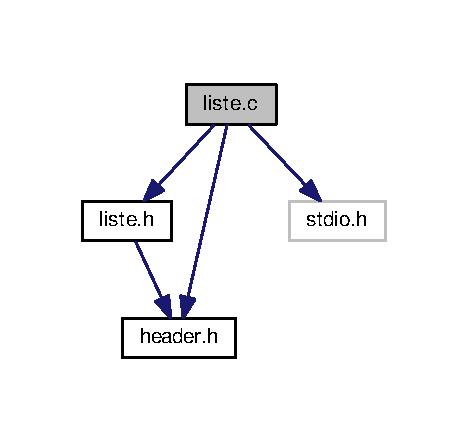
\includegraphics[width=225pt]{liste_8c__incl}
\end{center}
\end{figure}
\subsection*{Macros}
\begin{DoxyCompactItemize}
\item 
\#define \hyperlink{liste_8c_a31f3788284a4b6e361baa5bb3142c852}{N\+\_\+\+L\+I\+S\+T\+E}~100
\end{DoxyCompactItemize}
\subsection*{Fonctions}
\begin{DoxyCompactItemize}
\item 
void \hyperlink{liste_8c_aa325493a520928cd959f5cf829747b1c}{liste\+\_\+init} (void)
\item 
int \hyperlink{liste_8c_a1e4d1c45ace210278d08fd886268a0e3}{liste\+\_\+est\+\_\+vide} (void)
\item 
int \hyperlink{liste_8c_ad4a1a49d8756b972708e0870f9420776}{liste\+\_\+est\+\_\+hors\+\_\+liste} (void)
\item 
void \hyperlink{liste_8c_a9cbc13cd82829b3541fae0c01209f963}{liste\+\_\+en\+\_\+tete} (void)
\item 
void \hyperlink{liste_8c_aaf16c3ff04ebc19da036b0332d82ccee}{liste\+\_\+en\+\_\+queue} (void)
\item 
void \hyperlink{liste_8c_ae62f982aac8059018f004e3a7e2e7f21}{liste\+\_\+precedent} (void)
\item 
void \hyperlink{liste_8c_a801cf7ec08fb2c6b1dceb32af4a46111}{liste\+\_\+suivant} (void)
\item 
void \hyperlink{liste_8c_a1ad09d74d2d4f3b298db6b834933d744}{liste\+\_\+valeur\+\_\+elt} (\hyperlink{structt__coord}{t\+\_\+coord} $\ast$e)
\item 
void \hyperlink{liste_8c_a0282305b4b91dc5376333ac820bdf995}{liste\+\_\+modif\+\_\+elt} (\hyperlink{structt__coord}{t\+\_\+coord} v)
\item 
void \hyperlink{liste_8c_ac46b950926c8191e47c3822c624d2e1d}{liste\+\_\+oter\+\_\+elt} (void)
\item 
void \hyperlink{liste_8c_ae9c711baf0f41d27a5002c3e249687d8}{liste\+\_\+ajout\+\_\+droit} (\hyperlink{structt__coord}{t\+\_\+coord} e)
\item 
void \hyperlink{liste_8c_ac7289b3f288aec0c22e5272c4851e0ee}{liste\+\_\+ajout\+\_\+gauche} (\hyperlink{structt__coord}{t\+\_\+coord} e)
\item 
void \hyperlink{liste_8c_a207cdf13008fdfbf84b897ca499e3b17}{liste\+\_\+afficher\+\_\+contenu} ()
\item 
void \hyperlink{liste_8c_aeca8ab6b8935bc5fd81fa7a74e64879a}{liste\+\_\+afficher\+\_\+queue} ()
\item 
void \hyperlink{liste_8c_a48218f7c1bafab1e92490a0963ee7451}{liste\+\_\+suppr\+\_\+doublon} ()
\item 
int \hyperlink{liste_8c_a78de7382315436cf196cf30aac14257c}{liste\+\_\+calculer\+\_\+nombre\+\_\+elements} ()
\item 
int \hyperlink{liste_8c_ae6bf3307184d2f80167abcb9c2ad5b2b}{liste\+\_\+element\+\_\+est\+\_\+present} (\hyperlink{structt__coord}{t\+\_\+coord} e, int num\+Pile)
\end{DoxyCompactItemize}
\subsection*{Variables}
\begin{DoxyCompactItemize}
\item 
\hyperlink{structt__coord}{t\+\_\+coord} \hyperlink{liste_8c_a2d81e4bfb1b218a3e54b070304646b7c}{T} \mbox{[}\hyperlink{liste_8c_a31f3788284a4b6e361baa5bb3142c852}{N\+\_\+\+L\+I\+S\+T\+E}\mbox{]}
\item 
int \hyperlink{liste_8c_a404442353660d7effc914ba8220ebf7f}{queue}
\item 
int \hyperlink{liste_8c_a59e5dec85b6fd6e9ce7498410e234982}{ec}
\end{DoxyCompactItemize}


\subsection{Documentation des macros}
\hypertarget{liste_8c_a31f3788284a4b6e361baa5bb3142c852}{\index{liste.\+c@{liste.\+c}!N\+\_\+\+L\+I\+S\+T\+E@{N\+\_\+\+L\+I\+S\+T\+E}}
\index{N\+\_\+\+L\+I\+S\+T\+E@{N\+\_\+\+L\+I\+S\+T\+E}!liste.\+c@{liste.\+c}}
\subsubsection[{N\+\_\+\+L\+I\+S\+T\+E}]{\setlength{\rightskip}{0pt plus 5cm}\#define N\+\_\+\+L\+I\+S\+T\+E~100}}\label{liste_8c_a31f3788284a4b6e361baa5bb3142c852}


Définition à la ligne 2 du fichier liste.\+c.



\subsection{Documentation des fonctions}
\hypertarget{liste_8c_a207cdf13008fdfbf84b897ca499e3b17}{\index{liste.\+c@{liste.\+c}!liste\+\_\+afficher\+\_\+contenu@{liste\+\_\+afficher\+\_\+contenu}}
\index{liste\+\_\+afficher\+\_\+contenu@{liste\+\_\+afficher\+\_\+contenu}!liste.\+c@{liste.\+c}}
\subsubsection[{liste\+\_\+afficher\+\_\+contenu}]{\setlength{\rightskip}{0pt plus 5cm}void liste\+\_\+afficher\+\_\+contenu (
\begin{DoxyParamCaption}
{}
\end{DoxyParamCaption}
)}}\label{liste_8c_a207cdf13008fdfbf84b897ca499e3b17}


Définition à la ligne 120 du fichier liste.\+c.



Voici le graphe d'appel pour cette fonction \+:
\nopagebreak
\begin{figure}[H]
\begin{center}
\leavevmode
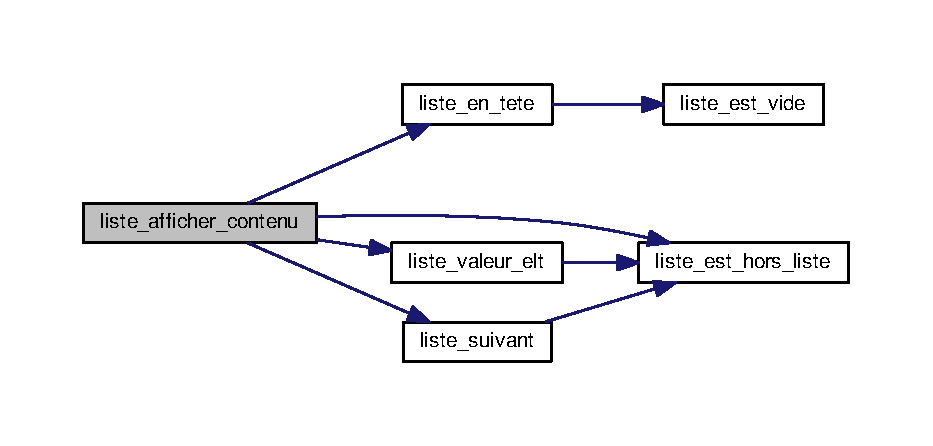
\includegraphics[width=350pt]{liste_8c_a207cdf13008fdfbf84b897ca499e3b17_cgraph}
\end{center}
\end{figure}


\hypertarget{liste_8c_aeca8ab6b8935bc5fd81fa7a74e64879a}{\index{liste.\+c@{liste.\+c}!liste\+\_\+afficher\+\_\+queue@{liste\+\_\+afficher\+\_\+queue}}
\index{liste\+\_\+afficher\+\_\+queue@{liste\+\_\+afficher\+\_\+queue}!liste.\+c@{liste.\+c}}
\subsubsection[{liste\+\_\+afficher\+\_\+queue}]{\setlength{\rightskip}{0pt plus 5cm}void liste\+\_\+afficher\+\_\+queue (
\begin{DoxyParamCaption}
{}
\end{DoxyParamCaption}
)}}\label{liste_8c_aeca8ab6b8935bc5fd81fa7a74e64879a}


Définition à la ligne 134 du fichier liste.\+c.



Voici le graphe d'appel pour cette fonction \+:
\nopagebreak
\begin{figure}[H]
\begin{center}
\leavevmode
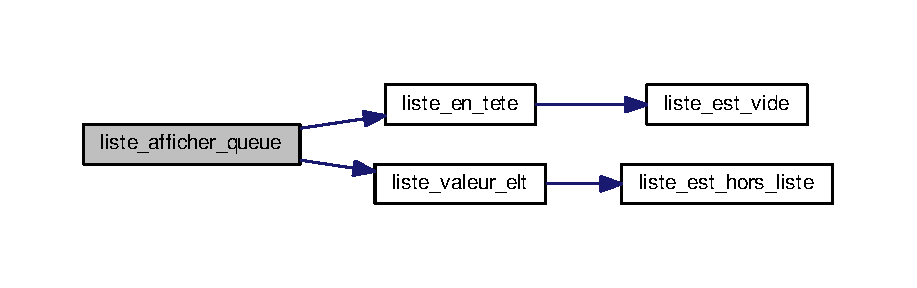
\includegraphics[width=350pt]{liste_8c_aeca8ab6b8935bc5fd81fa7a74e64879a_cgraph}
\end{center}
\end{figure}


\hypertarget{liste_8c_ae9c711baf0f41d27a5002c3e249687d8}{\index{liste.\+c@{liste.\+c}!liste\+\_\+ajout\+\_\+droit@{liste\+\_\+ajout\+\_\+droit}}
\index{liste\+\_\+ajout\+\_\+droit@{liste\+\_\+ajout\+\_\+droit}!liste.\+c@{liste.\+c}}
\subsubsection[{liste\+\_\+ajout\+\_\+droit}]{\setlength{\rightskip}{0pt plus 5cm}void liste\+\_\+ajout\+\_\+droit (
\begin{DoxyParamCaption}
\item[{{\bf t\+\_\+coord}}]{e}
\end{DoxyParamCaption}
)}}\label{liste_8c_ae9c711baf0f41d27a5002c3e249687d8}


Définition à la ligne 85 du fichier liste.\+c.



Voici le graphe d'appel pour cette fonction \+:
\nopagebreak
\begin{figure}[H]
\begin{center}
\leavevmode
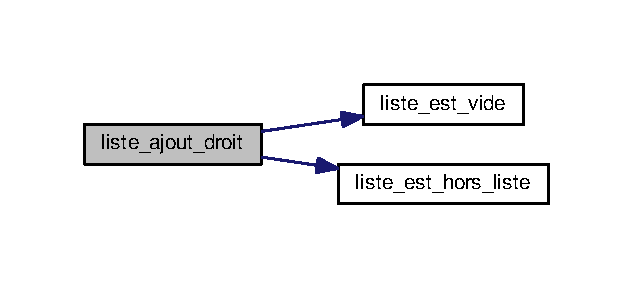
\includegraphics[width=304pt]{liste_8c_ae9c711baf0f41d27a5002c3e249687d8_cgraph}
\end{center}
\end{figure}




Voici le graphe des appelants de cette fonction \+:
\nopagebreak
\begin{figure}[H]
\begin{center}
\leavevmode
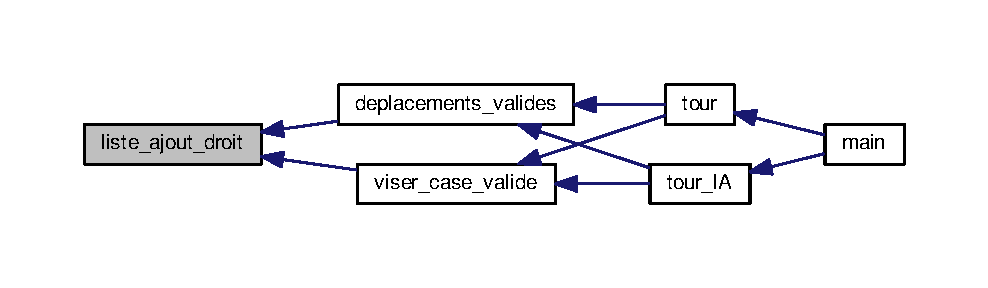
\includegraphics[width=350pt]{liste_8c_ae9c711baf0f41d27a5002c3e249687d8_icgraph}
\end{center}
\end{figure}


\hypertarget{liste_8c_ac7289b3f288aec0c22e5272c4851e0ee}{\index{liste.\+c@{liste.\+c}!liste\+\_\+ajout\+\_\+gauche@{liste\+\_\+ajout\+\_\+gauche}}
\index{liste\+\_\+ajout\+\_\+gauche@{liste\+\_\+ajout\+\_\+gauche}!liste.\+c@{liste.\+c}}
\subsubsection[{liste\+\_\+ajout\+\_\+gauche}]{\setlength{\rightskip}{0pt plus 5cm}void liste\+\_\+ajout\+\_\+gauche (
\begin{DoxyParamCaption}
\item[{{\bf t\+\_\+coord}}]{e}
\end{DoxyParamCaption}
)}}\label{liste_8c_ac7289b3f288aec0c22e5272c4851e0ee}


Définition à la ligne 103 du fichier liste.\+c.



Voici le graphe d'appel pour cette fonction \+:
\nopagebreak
\begin{figure}[H]
\begin{center}
\leavevmode
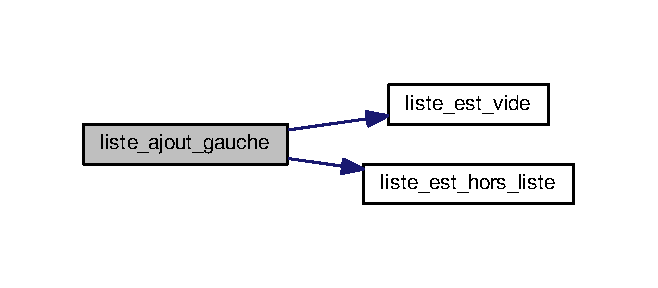
\includegraphics[width=316pt]{liste_8c_ac7289b3f288aec0c22e5272c4851e0ee_cgraph}
\end{center}
\end{figure}


\hypertarget{liste_8c_a78de7382315436cf196cf30aac14257c}{\index{liste.\+c@{liste.\+c}!liste\+\_\+calculer\+\_\+nombre\+\_\+elements@{liste\+\_\+calculer\+\_\+nombre\+\_\+elements}}
\index{liste\+\_\+calculer\+\_\+nombre\+\_\+elements@{liste\+\_\+calculer\+\_\+nombre\+\_\+elements}!liste.\+c@{liste.\+c}}
\subsubsection[{liste\+\_\+calculer\+\_\+nombre\+\_\+elements}]{\setlength{\rightskip}{0pt plus 5cm}int liste\+\_\+calculer\+\_\+nombre\+\_\+elements (
\begin{DoxyParamCaption}
{}
\end{DoxyParamCaption}
)}}\label{liste_8c_a78de7382315436cf196cf30aac14257c}


Définition à la ligne 167 du fichier liste.\+c.



Voici le graphe d'appel pour cette fonction \+:
\nopagebreak
\begin{figure}[H]
\begin{center}
\leavevmode
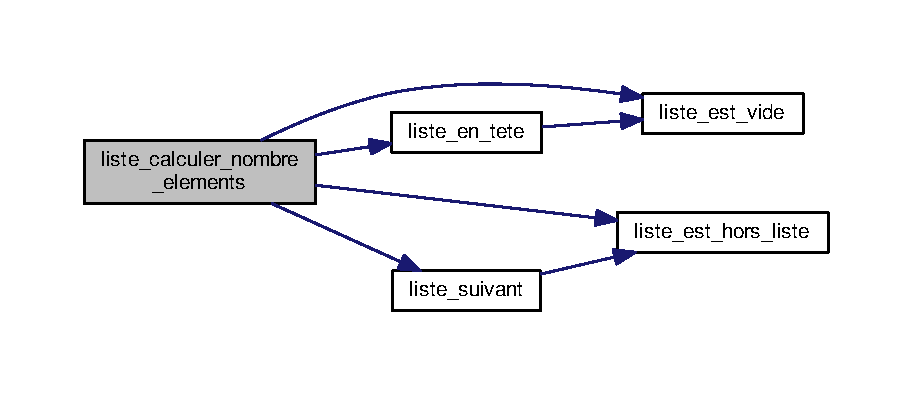
\includegraphics[width=350pt]{liste_8c_a78de7382315436cf196cf30aac14257c_cgraph}
\end{center}
\end{figure}




Voici le graphe des appelants de cette fonction \+:
\nopagebreak
\begin{figure}[H]
\begin{center}
\leavevmode
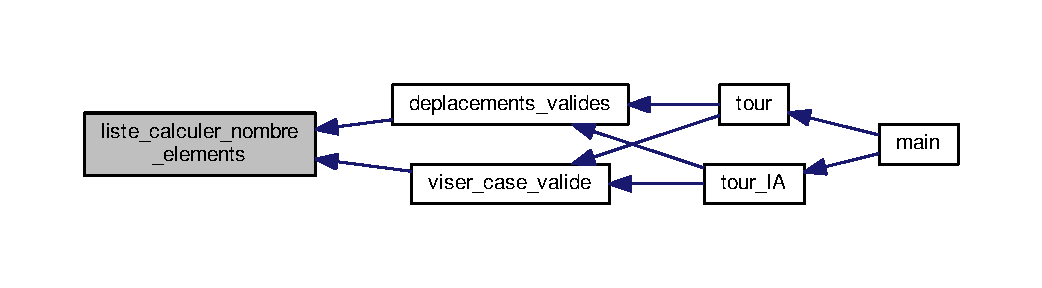
\includegraphics[width=350pt]{liste_8c_a78de7382315436cf196cf30aac14257c_icgraph}
\end{center}
\end{figure}


\hypertarget{liste_8c_ae6bf3307184d2f80167abcb9c2ad5b2b}{\index{liste.\+c@{liste.\+c}!liste\+\_\+element\+\_\+est\+\_\+present@{liste\+\_\+element\+\_\+est\+\_\+present}}
\index{liste\+\_\+element\+\_\+est\+\_\+present@{liste\+\_\+element\+\_\+est\+\_\+present}!liste.\+c@{liste.\+c}}
\subsubsection[{liste\+\_\+element\+\_\+est\+\_\+present}]{\setlength{\rightskip}{0pt plus 5cm}int liste\+\_\+element\+\_\+est\+\_\+present (
\begin{DoxyParamCaption}
\item[{{\bf t\+\_\+coord}}]{e, }
\item[{int}]{num\+Pile}
\end{DoxyParamCaption}
)}}\label{liste_8c_ae6bf3307184d2f80167abcb9c2ad5b2b}


Définition à la ligne 182 du fichier liste.\+c.



Voici le graphe d'appel pour cette fonction \+:
\nopagebreak
\begin{figure}[H]
\begin{center}
\leavevmode
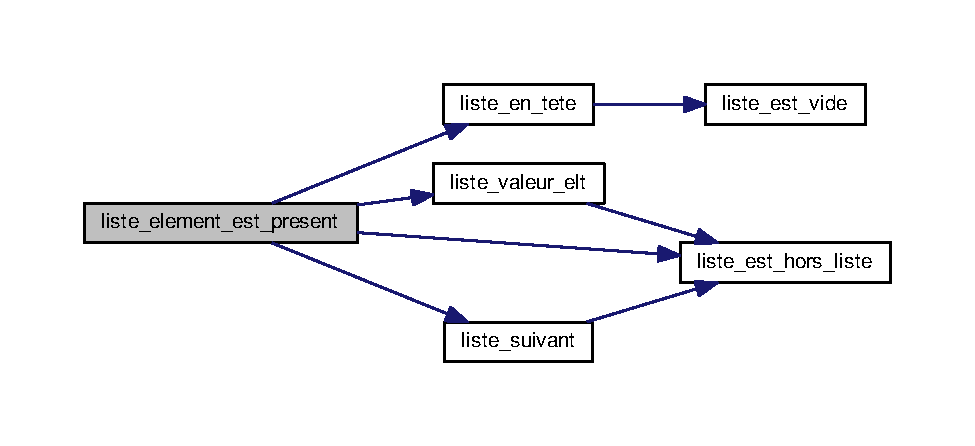
\includegraphics[width=350pt]{liste_8c_ae6bf3307184d2f80167abcb9c2ad5b2b_cgraph}
\end{center}
\end{figure}




Voici le graphe des appelants de cette fonction \+:
\nopagebreak
\begin{figure}[H]
\begin{center}
\leavevmode
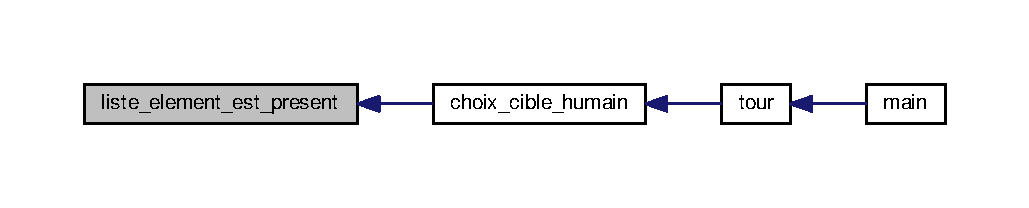
\includegraphics[width=350pt]{liste_8c_ae6bf3307184d2f80167abcb9c2ad5b2b_icgraph}
\end{center}
\end{figure}


\hypertarget{liste_8c_aaf16c3ff04ebc19da036b0332d82ccee}{\index{liste.\+c@{liste.\+c}!liste\+\_\+en\+\_\+queue@{liste\+\_\+en\+\_\+queue}}
\index{liste\+\_\+en\+\_\+queue@{liste\+\_\+en\+\_\+queue}!liste.\+c@{liste.\+c}}
\subsubsection[{liste\+\_\+en\+\_\+queue}]{\setlength{\rightskip}{0pt plus 5cm}void liste\+\_\+en\+\_\+queue (
\begin{DoxyParamCaption}
\item[{void}]{}
\end{DoxyParamCaption}
)}}\label{liste_8c_aaf16c3ff04ebc19da036b0332d82ccee}


Définition à la ligne 38 du fichier liste.\+c.



Voici le graphe d'appel pour cette fonction \+:
\nopagebreak
\begin{figure}[H]
\begin{center}
\leavevmode
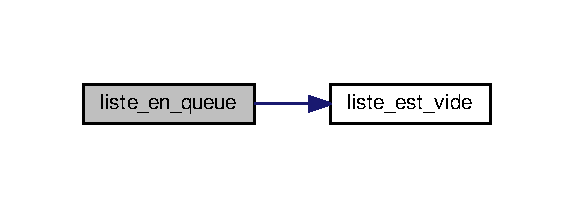
\includegraphics[width=276pt]{liste_8c_aaf16c3ff04ebc19da036b0332d82ccee_cgraph}
\end{center}
\end{figure}


\hypertarget{liste_8c_a9cbc13cd82829b3541fae0c01209f963}{\index{liste.\+c@{liste.\+c}!liste\+\_\+en\+\_\+tete@{liste\+\_\+en\+\_\+tete}}
\index{liste\+\_\+en\+\_\+tete@{liste\+\_\+en\+\_\+tete}!liste.\+c@{liste.\+c}}
\subsubsection[{liste\+\_\+en\+\_\+tete}]{\setlength{\rightskip}{0pt plus 5cm}void liste\+\_\+en\+\_\+tete (
\begin{DoxyParamCaption}
\item[{void}]{}
\end{DoxyParamCaption}
)}}\label{liste_8c_a9cbc13cd82829b3541fae0c01209f963}


Définition à la ligne 31 du fichier liste.\+c.



Voici le graphe d'appel pour cette fonction \+:
\nopagebreak
\begin{figure}[H]
\begin{center}
\leavevmode
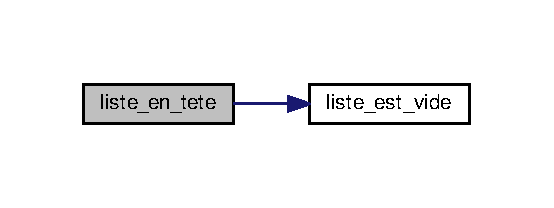
\includegraphics[width=266pt]{liste_8c_a9cbc13cd82829b3541fae0c01209f963_cgraph}
\end{center}
\end{figure}




Voici le graphe des appelants de cette fonction \+:
\nopagebreak
\begin{figure}[H]
\begin{center}
\leavevmode
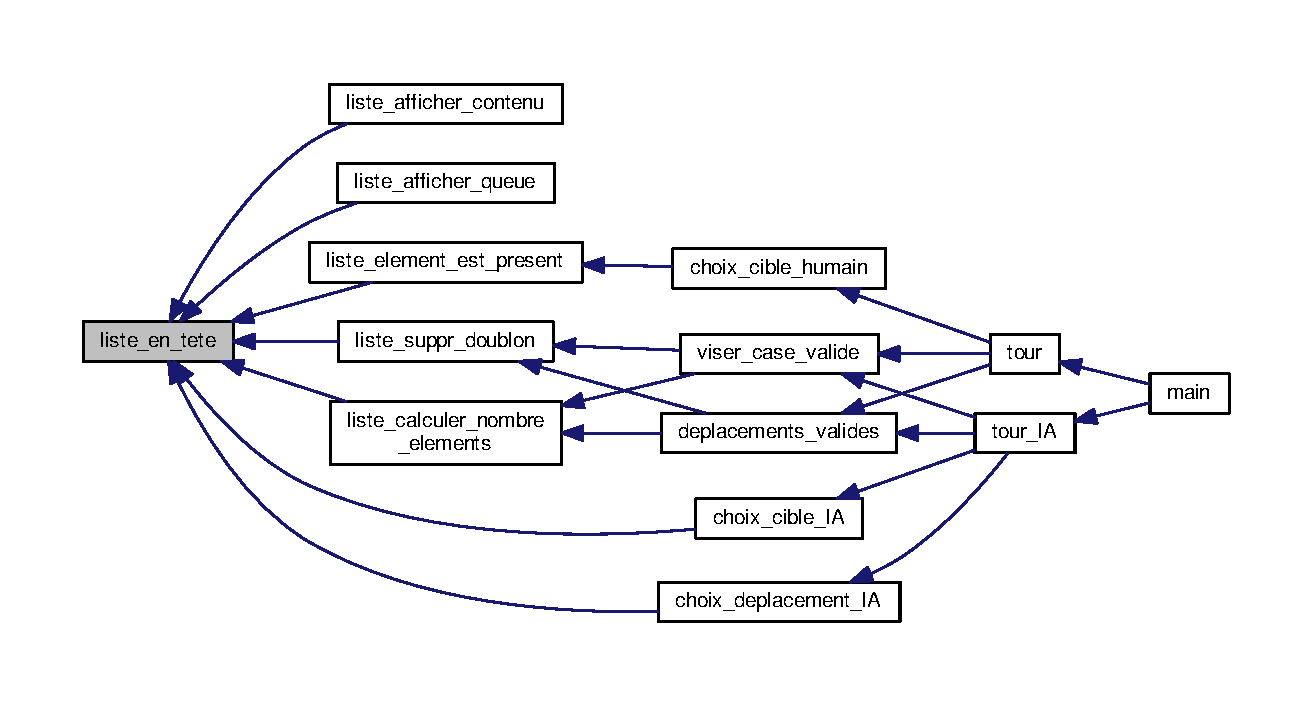
\includegraphics[width=350pt]{liste_8c_a9cbc13cd82829b3541fae0c01209f963_icgraph}
\end{center}
\end{figure}


\hypertarget{liste_8c_ad4a1a49d8756b972708e0870f9420776}{\index{liste.\+c@{liste.\+c}!liste\+\_\+est\+\_\+hors\+\_\+liste@{liste\+\_\+est\+\_\+hors\+\_\+liste}}
\index{liste\+\_\+est\+\_\+hors\+\_\+liste@{liste\+\_\+est\+\_\+hors\+\_\+liste}!liste.\+c@{liste.\+c}}
\subsubsection[{liste\+\_\+est\+\_\+hors\+\_\+liste}]{\setlength{\rightskip}{0pt plus 5cm}int liste\+\_\+est\+\_\+hors\+\_\+liste (
\begin{DoxyParamCaption}
\item[{void}]{}
\end{DoxyParamCaption}
)}}\label{liste_8c_ad4a1a49d8756b972708e0870f9420776}


Définition à la ligne 25 du fichier liste.\+c.



Voici le graphe des appelants de cette fonction \+:
\nopagebreak
\begin{figure}[H]
\begin{center}
\leavevmode
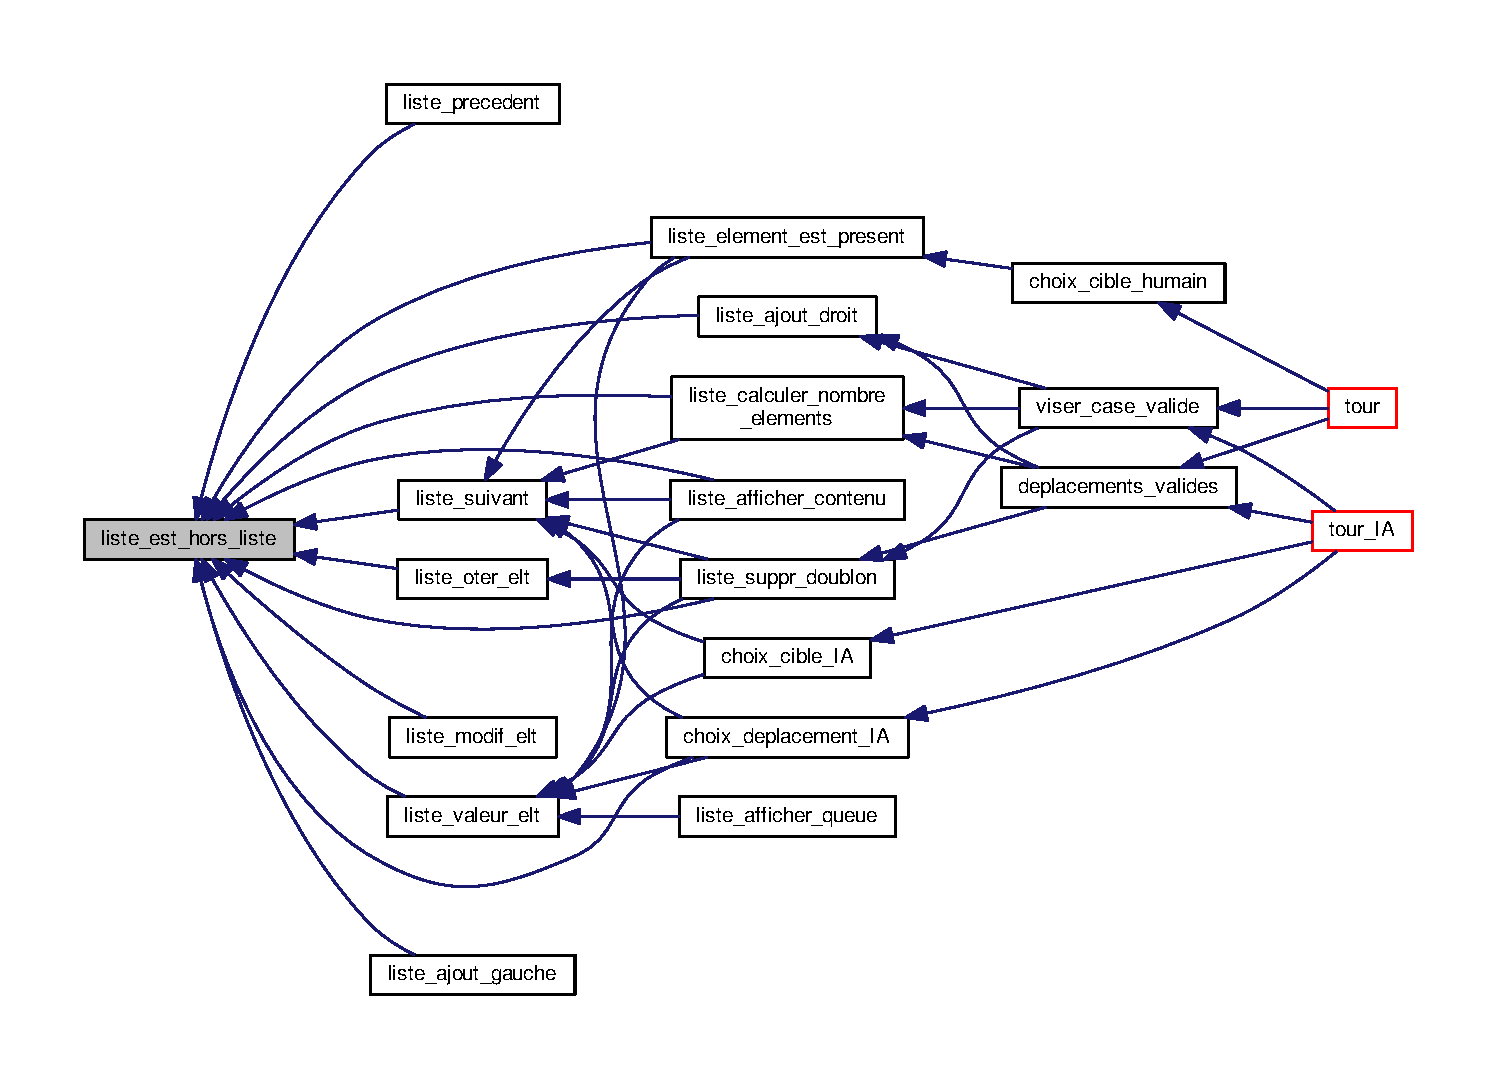
\includegraphics[width=350pt]{liste_8c_ad4a1a49d8756b972708e0870f9420776_icgraph}
\end{center}
\end{figure}


\hypertarget{liste_8c_a1e4d1c45ace210278d08fd886268a0e3}{\index{liste.\+c@{liste.\+c}!liste\+\_\+est\+\_\+vide@{liste\+\_\+est\+\_\+vide}}
\index{liste\+\_\+est\+\_\+vide@{liste\+\_\+est\+\_\+vide}!liste.\+c@{liste.\+c}}
\subsubsection[{liste\+\_\+est\+\_\+vide}]{\setlength{\rightskip}{0pt plus 5cm}int liste\+\_\+est\+\_\+vide (
\begin{DoxyParamCaption}
\item[{void}]{}
\end{DoxyParamCaption}
)}}\label{liste_8c_a1e4d1c45ace210278d08fd886268a0e3}


Définition à la ligne 19 du fichier liste.\+c.



Voici le graphe des appelants de cette fonction \+:
\nopagebreak
\begin{figure}[H]
\begin{center}
\leavevmode
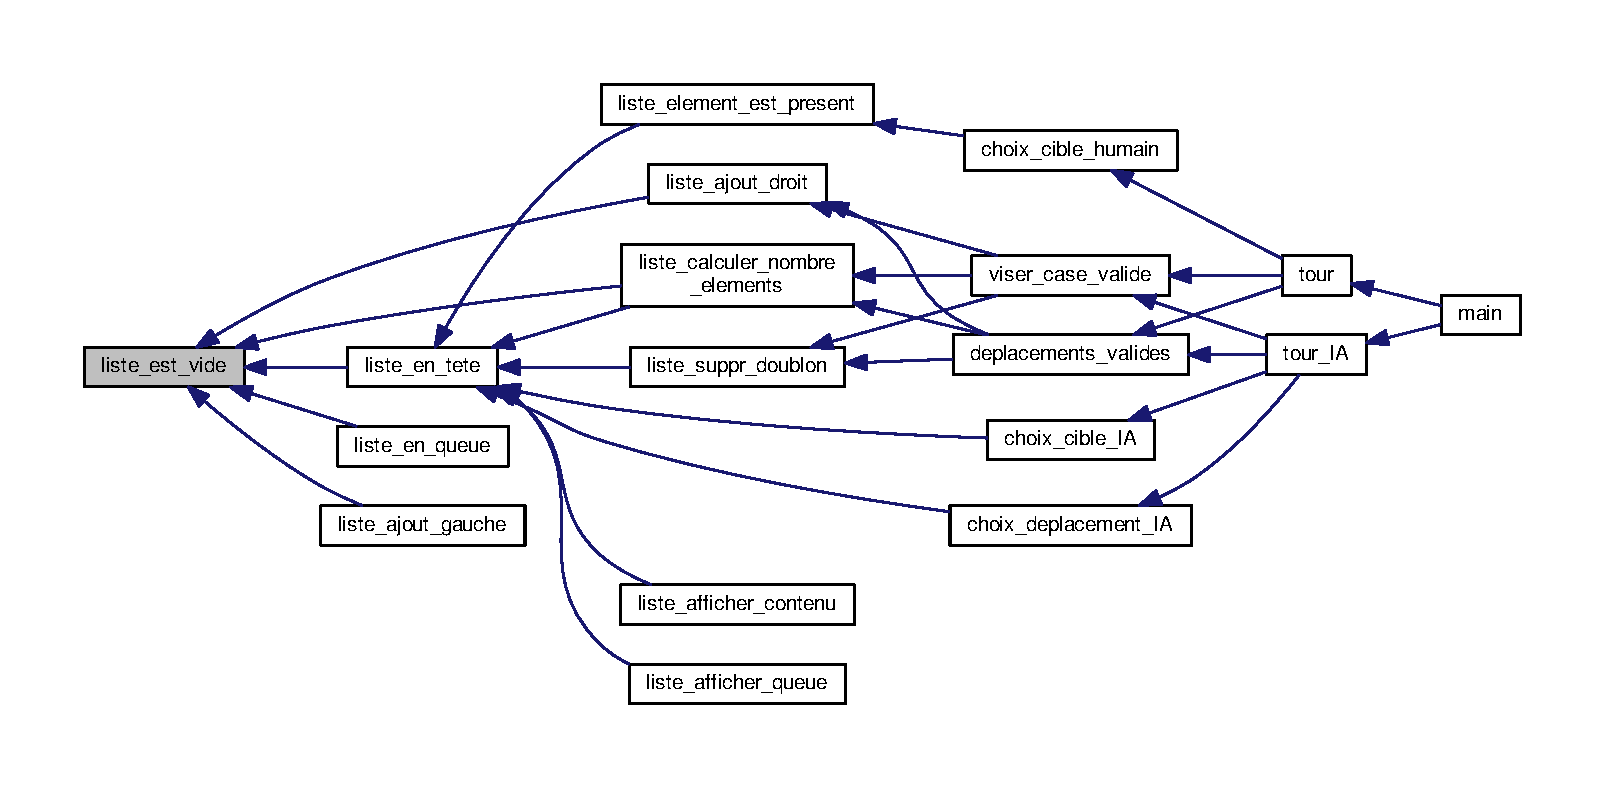
\includegraphics[width=350pt]{liste_8c_a1e4d1c45ace210278d08fd886268a0e3_icgraph}
\end{center}
\end{figure}


\hypertarget{liste_8c_aa325493a520928cd959f5cf829747b1c}{\index{liste.\+c@{liste.\+c}!liste\+\_\+init@{liste\+\_\+init}}
\index{liste\+\_\+init@{liste\+\_\+init}!liste.\+c@{liste.\+c}}
\subsubsection[{liste\+\_\+init}]{\setlength{\rightskip}{0pt plus 5cm}void liste\+\_\+init (
\begin{DoxyParamCaption}
\item[{void}]{}
\end{DoxyParamCaption}
)}}\label{liste_8c_aa325493a520928cd959f5cf829747b1c}


Définition à la ligne 12 du fichier liste.\+c.



Voici le graphe des appelants de cette fonction \+:
\nopagebreak
\begin{figure}[H]
\begin{center}
\leavevmode
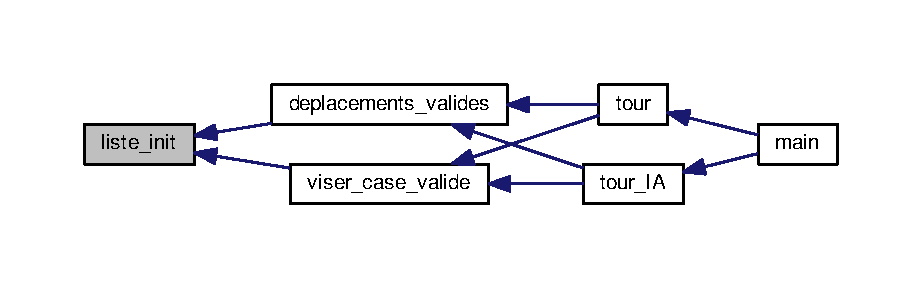
\includegraphics[width=350pt]{liste_8c_aa325493a520928cd959f5cf829747b1c_icgraph}
\end{center}
\end{figure}


\hypertarget{liste_8c_a0282305b4b91dc5376333ac820bdf995}{\index{liste.\+c@{liste.\+c}!liste\+\_\+modif\+\_\+elt@{liste\+\_\+modif\+\_\+elt}}
\index{liste\+\_\+modif\+\_\+elt@{liste\+\_\+modif\+\_\+elt}!liste.\+c@{liste.\+c}}
\subsubsection[{liste\+\_\+modif\+\_\+elt}]{\setlength{\rightskip}{0pt plus 5cm}void liste\+\_\+modif\+\_\+elt (
\begin{DoxyParamCaption}
\item[{{\bf t\+\_\+coord}}]{v}
\end{DoxyParamCaption}
)}}\label{liste_8c_a0282305b4b91dc5376333ac820bdf995}


Définition à la ligne 66 du fichier liste.\+c.



Voici le graphe d'appel pour cette fonction \+:
\nopagebreak
\begin{figure}[H]
\begin{center}
\leavevmode
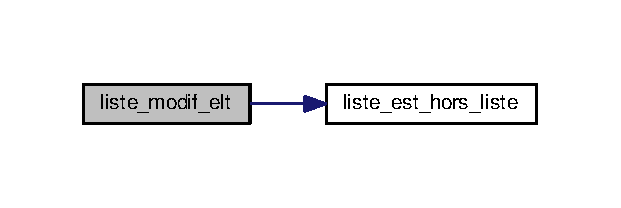
\includegraphics[width=298pt]{liste_8c_a0282305b4b91dc5376333ac820bdf995_cgraph}
\end{center}
\end{figure}


\hypertarget{liste_8c_ac46b950926c8191e47c3822c624d2e1d}{\index{liste.\+c@{liste.\+c}!liste\+\_\+oter\+\_\+elt@{liste\+\_\+oter\+\_\+elt}}
\index{liste\+\_\+oter\+\_\+elt@{liste\+\_\+oter\+\_\+elt}!liste.\+c@{liste.\+c}}
\subsubsection[{liste\+\_\+oter\+\_\+elt}]{\setlength{\rightskip}{0pt plus 5cm}void liste\+\_\+oter\+\_\+elt (
\begin{DoxyParamCaption}
\item[{void}]{}
\end{DoxyParamCaption}
)}}\label{liste_8c_ac46b950926c8191e47c3822c624d2e1d}


Définition à la ligne 73 du fichier liste.\+c.



Voici le graphe d'appel pour cette fonction \+:
\nopagebreak
\begin{figure}[H]
\begin{center}
\leavevmode
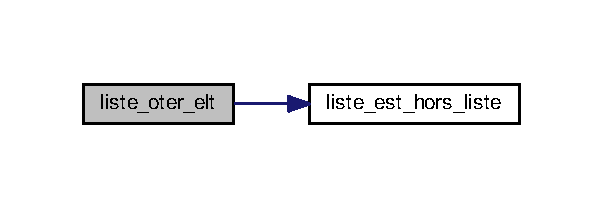
\includegraphics[width=290pt]{liste_8c_ac46b950926c8191e47c3822c624d2e1d_cgraph}
\end{center}
\end{figure}




Voici le graphe des appelants de cette fonction \+:
\nopagebreak
\begin{figure}[H]
\begin{center}
\leavevmode
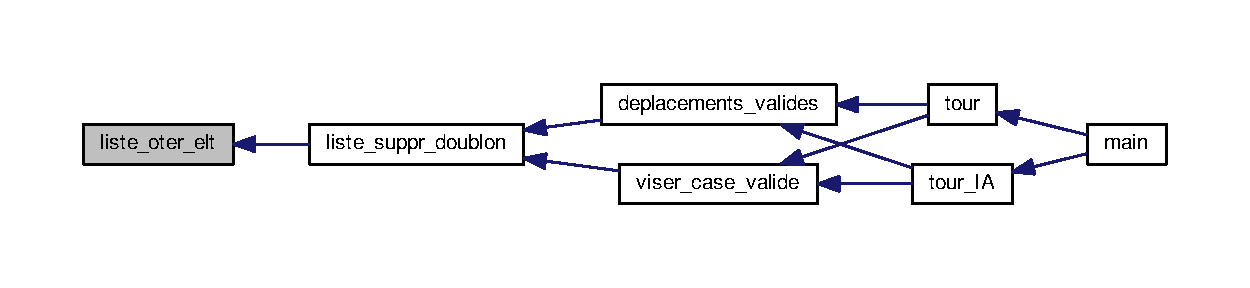
\includegraphics[width=350pt]{liste_8c_ac46b950926c8191e47c3822c624d2e1d_icgraph}
\end{center}
\end{figure}


\hypertarget{liste_8c_ae62f982aac8059018f004e3a7e2e7f21}{\index{liste.\+c@{liste.\+c}!liste\+\_\+precedent@{liste\+\_\+precedent}}
\index{liste\+\_\+precedent@{liste\+\_\+precedent}!liste.\+c@{liste.\+c}}
\subsubsection[{liste\+\_\+precedent}]{\setlength{\rightskip}{0pt plus 5cm}void liste\+\_\+precedent (
\begin{DoxyParamCaption}
\item[{void}]{}
\end{DoxyParamCaption}
)}}\label{liste_8c_ae62f982aac8059018f004e3a7e2e7f21}


Définition à la ligne 45 du fichier liste.\+c.



Voici le graphe d'appel pour cette fonction \+:
\nopagebreak
\begin{figure}[H]
\begin{center}
\leavevmode
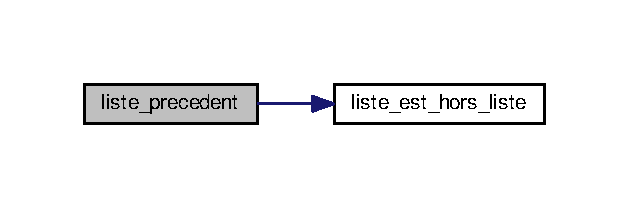
\includegraphics[width=302pt]{liste_8c_ae62f982aac8059018f004e3a7e2e7f21_cgraph}
\end{center}
\end{figure}


\hypertarget{liste_8c_a801cf7ec08fb2c6b1dceb32af4a46111}{\index{liste.\+c@{liste.\+c}!liste\+\_\+suivant@{liste\+\_\+suivant}}
\index{liste\+\_\+suivant@{liste\+\_\+suivant}!liste.\+c@{liste.\+c}}
\subsubsection[{liste\+\_\+suivant}]{\setlength{\rightskip}{0pt plus 5cm}void liste\+\_\+suivant (
\begin{DoxyParamCaption}
\item[{void}]{}
\end{DoxyParamCaption}
)}}\label{liste_8c_a801cf7ec08fb2c6b1dceb32af4a46111}


Définition à la ligne 52 du fichier liste.\+c.



Voici le graphe d'appel pour cette fonction \+:
\nopagebreak
\begin{figure}[H]
\begin{center}
\leavevmode
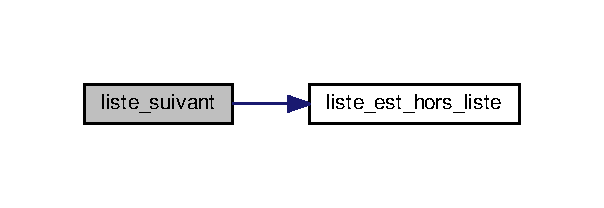
\includegraphics[width=290pt]{liste_8c_a801cf7ec08fb2c6b1dceb32af4a46111_cgraph}
\end{center}
\end{figure}




Voici le graphe des appelants de cette fonction \+:
\nopagebreak
\begin{figure}[H]
\begin{center}
\leavevmode
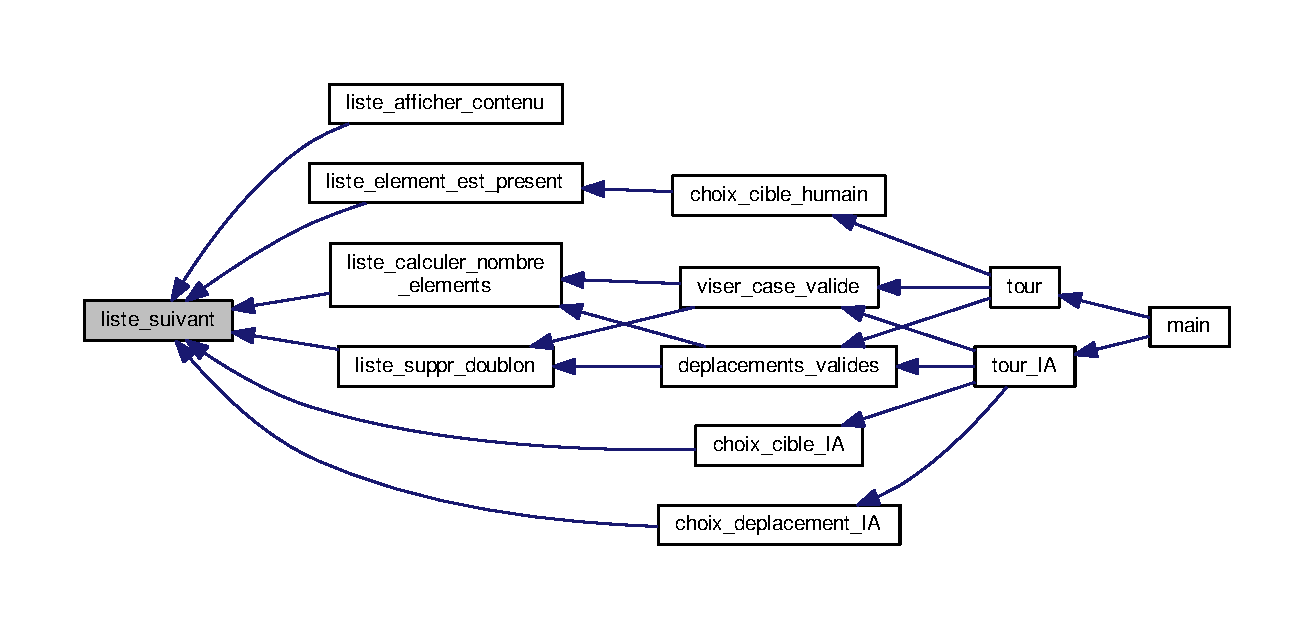
\includegraphics[width=350pt]{liste_8c_a801cf7ec08fb2c6b1dceb32af4a46111_icgraph}
\end{center}
\end{figure}


\hypertarget{liste_8c_a48218f7c1bafab1e92490a0963ee7451}{\index{liste.\+c@{liste.\+c}!liste\+\_\+suppr\+\_\+doublon@{liste\+\_\+suppr\+\_\+doublon}}
\index{liste\+\_\+suppr\+\_\+doublon@{liste\+\_\+suppr\+\_\+doublon}!liste.\+c@{liste.\+c}}
\subsubsection[{liste\+\_\+suppr\+\_\+doublon}]{\setlength{\rightskip}{0pt plus 5cm}void liste\+\_\+suppr\+\_\+doublon (
\begin{DoxyParamCaption}
{}
\end{DoxyParamCaption}
)}}\label{liste_8c_a48218f7c1bafab1e92490a0963ee7451}


Définition à la ligne 143 du fichier liste.\+c.



Voici le graphe d'appel pour cette fonction \+:
\nopagebreak
\begin{figure}[H]
\begin{center}
\leavevmode
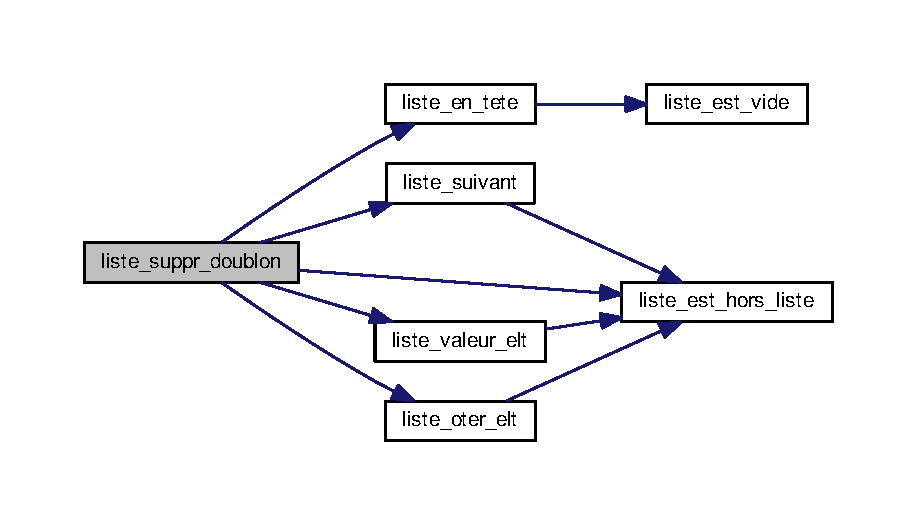
\includegraphics[width=350pt]{liste_8c_a48218f7c1bafab1e92490a0963ee7451_cgraph}
\end{center}
\end{figure}




Voici le graphe des appelants de cette fonction \+:
\nopagebreak
\begin{figure}[H]
\begin{center}
\leavevmode
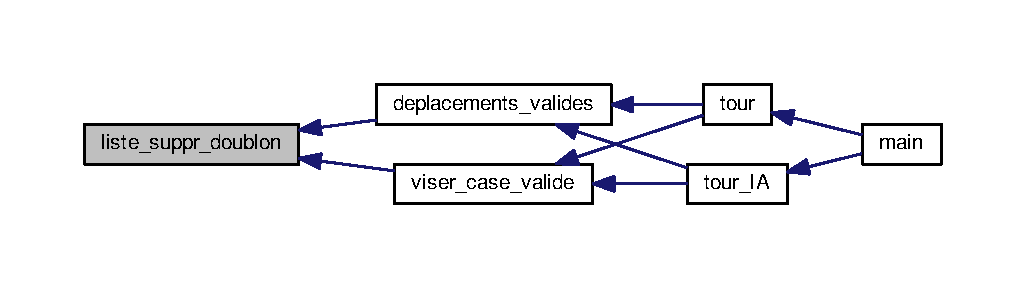
\includegraphics[width=350pt]{liste_8c_a48218f7c1bafab1e92490a0963ee7451_icgraph}
\end{center}
\end{figure}


\hypertarget{liste_8c_a1ad09d74d2d4f3b298db6b834933d744}{\index{liste.\+c@{liste.\+c}!liste\+\_\+valeur\+\_\+elt@{liste\+\_\+valeur\+\_\+elt}}
\index{liste\+\_\+valeur\+\_\+elt@{liste\+\_\+valeur\+\_\+elt}!liste.\+c@{liste.\+c}}
\subsubsection[{liste\+\_\+valeur\+\_\+elt}]{\setlength{\rightskip}{0pt plus 5cm}void liste\+\_\+valeur\+\_\+elt (
\begin{DoxyParamCaption}
\item[{{\bf t\+\_\+coord} $\ast$}]{e}
\end{DoxyParamCaption}
)}}\label{liste_8c_a1ad09d74d2d4f3b298db6b834933d744}


Définition à la ligne 59 du fichier liste.\+c.



Voici le graphe d'appel pour cette fonction \+:
\nopagebreak
\begin{figure}[H]
\begin{center}
\leavevmode
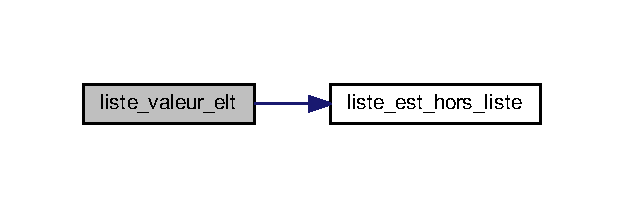
\includegraphics[width=300pt]{liste_8c_a1ad09d74d2d4f3b298db6b834933d744_cgraph}
\end{center}
\end{figure}




Voici le graphe des appelants de cette fonction \+:
\nopagebreak
\begin{figure}[H]
\begin{center}
\leavevmode
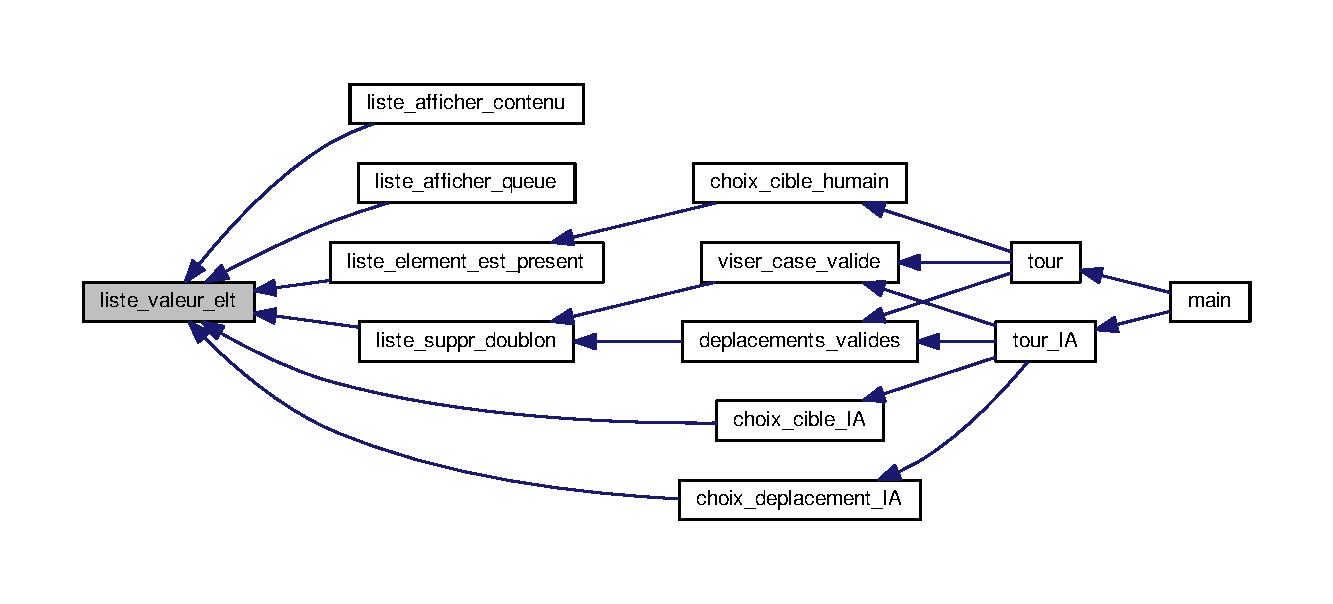
\includegraphics[width=350pt]{liste_8c_a1ad09d74d2d4f3b298db6b834933d744_icgraph}
\end{center}
\end{figure}




\subsection{Documentation des variables}
\hypertarget{liste_8c_a59e5dec85b6fd6e9ce7498410e234982}{\index{liste.\+c@{liste.\+c}!ec@{ec}}
\index{ec@{ec}!liste.\+c@{liste.\+c}}
\subsubsection[{ec}]{\setlength{\rightskip}{0pt plus 5cm}int ec}}\label{liste_8c_a59e5dec85b6fd6e9ce7498410e234982}


Définition à la ligne 10 du fichier liste.\+c.

\hypertarget{liste_8c_a404442353660d7effc914ba8220ebf7f}{\index{liste.\+c@{liste.\+c}!queue@{queue}}
\index{queue@{queue}!liste.\+c@{liste.\+c}}
\subsubsection[{queue}]{\setlength{\rightskip}{0pt plus 5cm}int queue}}\label{liste_8c_a404442353660d7effc914ba8220ebf7f}


Définition à la ligne 10 du fichier liste.\+c.

\hypertarget{liste_8c_a2d81e4bfb1b218a3e54b070304646b7c}{\index{liste.\+c@{liste.\+c}!T@{T}}
\index{T@{T}!liste.\+c@{liste.\+c}}
\subsubsection[{T}]{\setlength{\rightskip}{0pt plus 5cm}{\bf t\+\_\+coord} T\mbox{[}{\bf N\+\_\+\+L\+I\+S\+T\+E}\mbox{]}}}\label{liste_8c_a2d81e4bfb1b218a3e54b070304646b7c}


Définition à la ligne 8 du fichier liste.\+c.


\hypertarget{liste_8h}{\section{liste.\-h File Reference}
\label{liste_8h}\index{liste.\-h@{liste.\-h}}
}
{\ttfamily \#include \char`\"{}header.\-h\char`\"{}}\\*
Include dependency graph for liste.\-h\-:
\nopagebreak
\begin{figure}[H]
\begin{center}
\leavevmode
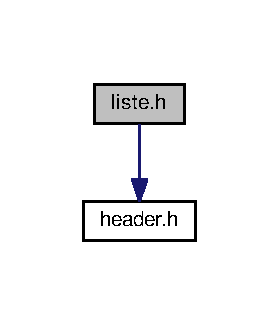
\includegraphics[width=134pt]{liste_8h__incl}
\end{center}
\end{figure}
This graph shows which files directly or indirectly include this file\-:
\nopagebreak
\begin{figure}[H]
\begin{center}
\leavevmode
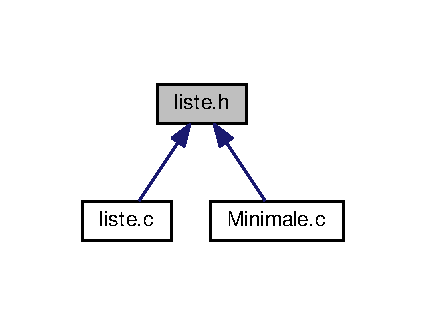
\includegraphics[width=205pt]{liste_8h__dep__incl}
\end{center}
\end{figure}
\subsection*{Functions}
\begin{DoxyCompactItemize}
\item 
$<$$<$$<$$<$$<$$<$$<$ H\-E\-A\-D=======$>$$>$$>$$>$$>$$>$ void \hyperlink{liste_8h_a522697519e93e19d07943667b472a5c1}{liste\-\_\-init} (void)
\item 
int \hyperlink{liste_8h_a1e4d1c45ace210278d08fd886268a0e3}{liste\-\_\-est\-\_\-vide} (void)
\item 
int \hyperlink{liste_8h_ad4a1a49d8756b972708e0870f9420776}{liste\-\_\-est\-\_\-hors\-\_\-liste} (void)
\item 
void \hyperlink{liste_8h_a9cbc13cd82829b3541fae0c01209f963}{liste\-\_\-en\-\_\-tete} (void)
\item 
void \hyperlink{liste_8h_aaf16c3ff04ebc19da036b0332d82ccee}{liste\-\_\-en\-\_\-queue} (void)
\item 
void \hyperlink{liste_8h_ae62f982aac8059018f004e3a7e2e7f21}{liste\-\_\-precedent} (void)
\item 
void \hyperlink{liste_8h_a801cf7ec08fb2c6b1dceb32af4a46111}{liste\-\_\-suivant} (void)
\item 
void \hyperlink{liste_8h_a1ad09d74d2d4f3b298db6b834933d744}{liste\-\_\-valeur\-\_\-elt} (\hyperlink{structt__coord}{t\-\_\-coord} $\ast$e)
\item 
void \hyperlink{liste_8h_a0282305b4b91dc5376333ac820bdf995}{liste\-\_\-modif\-\_\-elt} (\hyperlink{structt__coord}{t\-\_\-coord} v)
\item 
void \hyperlink{liste_8h_ac46b950926c8191e47c3822c624d2e1d}{liste\-\_\-oter\-\_\-elt} (void)
\item 
void \hyperlink{liste_8h_ae9c711baf0f41d27a5002c3e249687d8}{liste\-\_\-ajout\-\_\-droit} (\hyperlink{structt__coord}{t\-\_\-coord} e)
\item 
void \hyperlink{liste_8h_ac7289b3f288aec0c22e5272c4851e0ee}{liste\-\_\-ajout\-\_\-gauche} (\hyperlink{structt__coord}{t\-\_\-coord} e)
\item 
void \hyperlink{liste_8h_a207cdf13008fdfbf84b897ca499e3b17}{liste\-\_\-afficher\-\_\-contenu} ()
\item 
void \hyperlink{liste_8h_aeca8ab6b8935bc5fd81fa7a74e64879a}{liste\-\_\-afficher\-\_\-queue} ()
\item 
void \hyperlink{liste_8h_a48218f7c1bafab1e92490a0963ee7451}{liste\-\_\-suppr\-\_\-doublon} ()
\item 
int \hyperlink{liste_8h_a78de7382315436cf196cf30aac14257c}{liste\-\_\-calculer\-\_\-nombre\-\_\-elements} ()
\end{DoxyCompactItemize}


\subsection{Function Documentation}
\hypertarget{liste_8h_a207cdf13008fdfbf84b897ca499e3b17}{\index{liste.\-h@{liste.\-h}!liste\-\_\-afficher\-\_\-contenu@{liste\-\_\-afficher\-\_\-contenu}}
\index{liste\-\_\-afficher\-\_\-contenu@{liste\-\_\-afficher\-\_\-contenu}!liste.h@{liste.\-h}}
\subsubsection[{liste\-\_\-afficher\-\_\-contenu}]{\setlength{\rightskip}{0pt plus 5cm}void liste\-\_\-afficher\-\_\-contenu (
\begin{DoxyParamCaption}
{}
\end{DoxyParamCaption}
)}}\label{liste_8h_a207cdf13008fdfbf84b897ca499e3b17}


Definition at line 120 of file liste.\-c.



Here is the call graph for this function\-:
\nopagebreak
\begin{figure}[H]
\begin{center}
\leavevmode
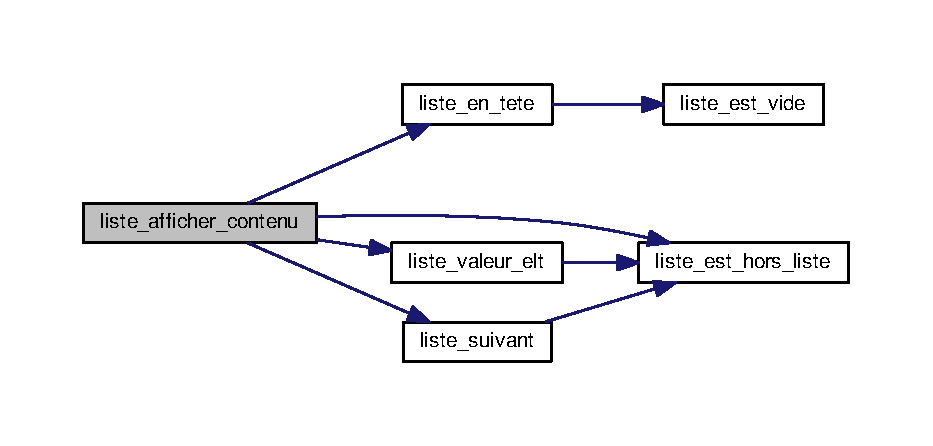
\includegraphics[width=350pt]{liste_8h_a207cdf13008fdfbf84b897ca499e3b17_cgraph}
\end{center}
\end{figure}


\hypertarget{liste_8h_aeca8ab6b8935bc5fd81fa7a74e64879a}{\index{liste.\-h@{liste.\-h}!liste\-\_\-afficher\-\_\-queue@{liste\-\_\-afficher\-\_\-queue}}
\index{liste\-\_\-afficher\-\_\-queue@{liste\-\_\-afficher\-\_\-queue}!liste.h@{liste.\-h}}
\subsubsection[{liste\-\_\-afficher\-\_\-queue}]{\setlength{\rightskip}{0pt plus 5cm}void liste\-\_\-afficher\-\_\-queue (
\begin{DoxyParamCaption}
{}
\end{DoxyParamCaption}
)}}\label{liste_8h_aeca8ab6b8935bc5fd81fa7a74e64879a}


Definition at line 134 of file liste.\-c.



Here is the call graph for this function\-:
\nopagebreak
\begin{figure}[H]
\begin{center}
\leavevmode
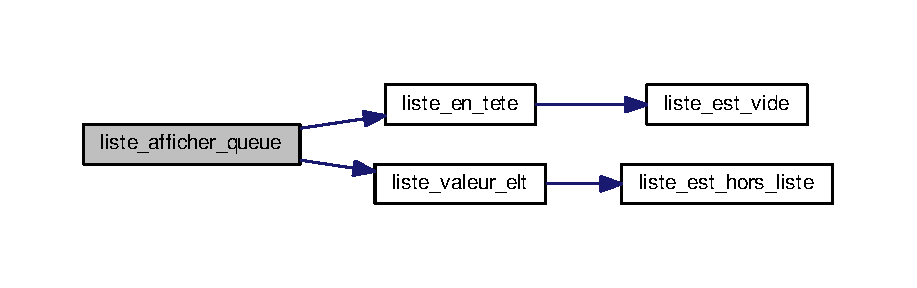
\includegraphics[width=350pt]{liste_8h_aeca8ab6b8935bc5fd81fa7a74e64879a_cgraph}
\end{center}
\end{figure}


\hypertarget{liste_8h_ae9c711baf0f41d27a5002c3e249687d8}{\index{liste.\-h@{liste.\-h}!liste\-\_\-ajout\-\_\-droit@{liste\-\_\-ajout\-\_\-droit}}
\index{liste\-\_\-ajout\-\_\-droit@{liste\-\_\-ajout\-\_\-droit}!liste.h@{liste.\-h}}
\subsubsection[{liste\-\_\-ajout\-\_\-droit}]{\setlength{\rightskip}{0pt plus 5cm}void liste\-\_\-ajout\-\_\-droit (
\begin{DoxyParamCaption}
\item[{{\bf t\-\_\-coord}}]{e}
\end{DoxyParamCaption}
)}}\label{liste_8h_ae9c711baf0f41d27a5002c3e249687d8}


Definition at line 85 of file liste.\-c.



Here is the call graph for this function\-:
\nopagebreak
\begin{figure}[H]
\begin{center}
\leavevmode
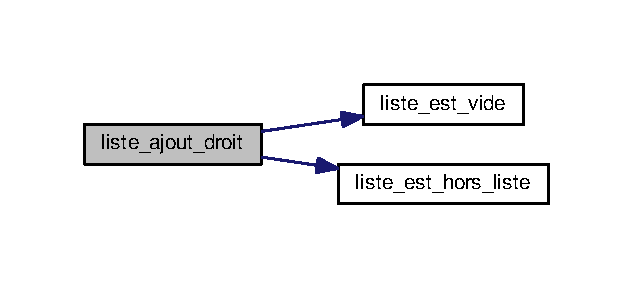
\includegraphics[width=304pt]{liste_8h_ae9c711baf0f41d27a5002c3e249687d8_cgraph}
\end{center}
\end{figure}




Here is the caller graph for this function\-:
\nopagebreak
\begin{figure}[H]
\begin{center}
\leavevmode
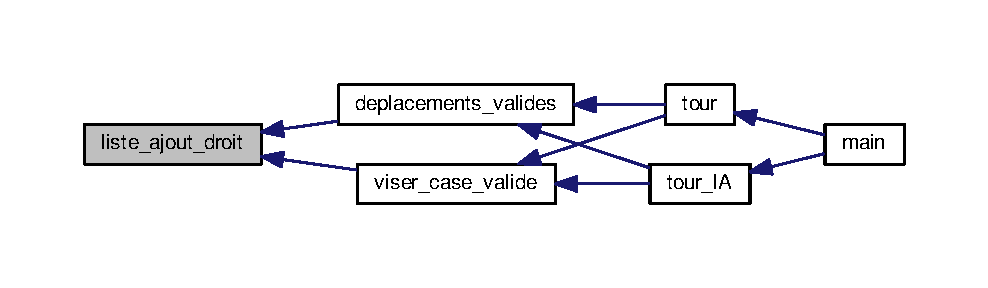
\includegraphics[width=350pt]{liste_8h_ae9c711baf0f41d27a5002c3e249687d8_icgraph}
\end{center}
\end{figure}


\hypertarget{liste_8h_ac7289b3f288aec0c22e5272c4851e0ee}{\index{liste.\-h@{liste.\-h}!liste\-\_\-ajout\-\_\-gauche@{liste\-\_\-ajout\-\_\-gauche}}
\index{liste\-\_\-ajout\-\_\-gauche@{liste\-\_\-ajout\-\_\-gauche}!liste.h@{liste.\-h}}
\subsubsection[{liste\-\_\-ajout\-\_\-gauche}]{\setlength{\rightskip}{0pt plus 5cm}void liste\-\_\-ajout\-\_\-gauche (
\begin{DoxyParamCaption}
\item[{{\bf t\-\_\-coord}}]{e}
\end{DoxyParamCaption}
)}}\label{liste_8h_ac7289b3f288aec0c22e5272c4851e0ee}


Definition at line 103 of file liste.\-c.



Here is the call graph for this function\-:
\nopagebreak
\begin{figure}[H]
\begin{center}
\leavevmode
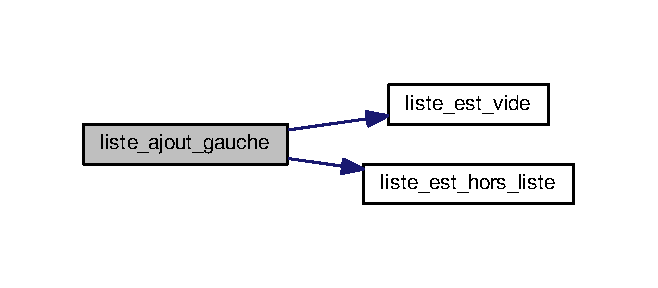
\includegraphics[width=316pt]{liste_8h_ac7289b3f288aec0c22e5272c4851e0ee_cgraph}
\end{center}
\end{figure}


\hypertarget{liste_8h_a78de7382315436cf196cf30aac14257c}{\index{liste.\-h@{liste.\-h}!liste\-\_\-calculer\-\_\-nombre\-\_\-elements@{liste\-\_\-calculer\-\_\-nombre\-\_\-elements}}
\index{liste\-\_\-calculer\-\_\-nombre\-\_\-elements@{liste\-\_\-calculer\-\_\-nombre\-\_\-elements}!liste.h@{liste.\-h}}
\subsubsection[{liste\-\_\-calculer\-\_\-nombre\-\_\-elements}]{\setlength{\rightskip}{0pt plus 5cm}int liste\-\_\-calculer\-\_\-nombre\-\_\-elements (
\begin{DoxyParamCaption}
{}
\end{DoxyParamCaption}
)}}\label{liste_8h_a78de7382315436cf196cf30aac14257c}


Definition at line 167 of file liste.\-c.



Here is the call graph for this function\-:
\nopagebreak
\begin{figure}[H]
\begin{center}
\leavevmode
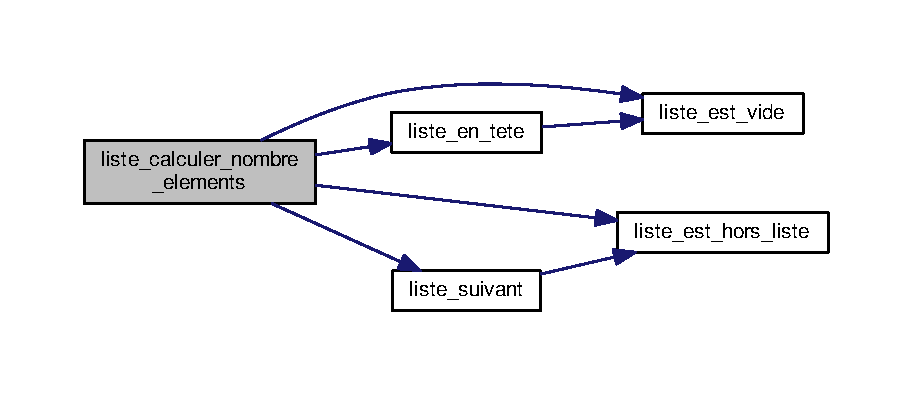
\includegraphics[width=350pt]{liste_8h_a78de7382315436cf196cf30aac14257c_cgraph}
\end{center}
\end{figure}




Here is the caller graph for this function\-:
\nopagebreak
\begin{figure}[H]
\begin{center}
\leavevmode
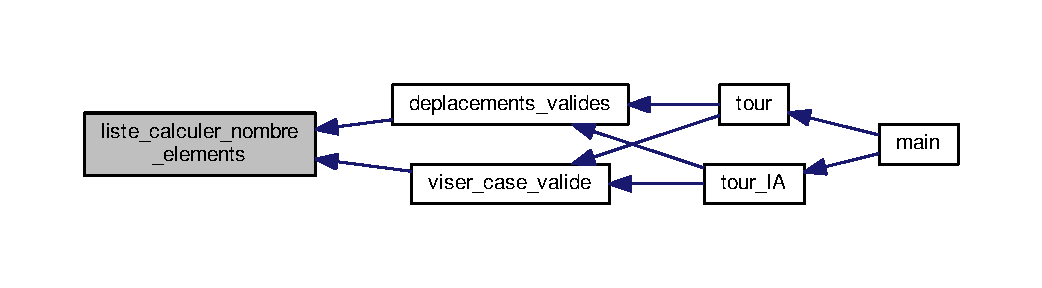
\includegraphics[width=350pt]{liste_8h_a78de7382315436cf196cf30aac14257c_icgraph}
\end{center}
\end{figure}


\hypertarget{liste_8h_aaf16c3ff04ebc19da036b0332d82ccee}{\index{liste.\-h@{liste.\-h}!liste\-\_\-en\-\_\-queue@{liste\-\_\-en\-\_\-queue}}
\index{liste\-\_\-en\-\_\-queue@{liste\-\_\-en\-\_\-queue}!liste.h@{liste.\-h}}
\subsubsection[{liste\-\_\-en\-\_\-queue}]{\setlength{\rightskip}{0pt plus 5cm}void liste\-\_\-en\-\_\-queue (
\begin{DoxyParamCaption}
\item[{void}]{}
\end{DoxyParamCaption}
)}}\label{liste_8h_aaf16c3ff04ebc19da036b0332d82ccee}


Definition at line 38 of file liste.\-c.



Here is the call graph for this function\-:
\nopagebreak
\begin{figure}[H]
\begin{center}
\leavevmode
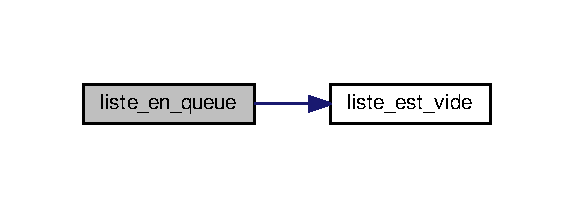
\includegraphics[width=276pt]{liste_8h_aaf16c3ff04ebc19da036b0332d82ccee_cgraph}
\end{center}
\end{figure}


\hypertarget{liste_8h_a9cbc13cd82829b3541fae0c01209f963}{\index{liste.\-h@{liste.\-h}!liste\-\_\-en\-\_\-tete@{liste\-\_\-en\-\_\-tete}}
\index{liste\-\_\-en\-\_\-tete@{liste\-\_\-en\-\_\-tete}!liste.h@{liste.\-h}}
\subsubsection[{liste\-\_\-en\-\_\-tete}]{\setlength{\rightskip}{0pt plus 5cm}void liste\-\_\-en\-\_\-tete (
\begin{DoxyParamCaption}
\item[{void}]{}
\end{DoxyParamCaption}
)}}\label{liste_8h_a9cbc13cd82829b3541fae0c01209f963}


Definition at line 31 of file liste.\-c.



Here is the call graph for this function\-:
\nopagebreak
\begin{figure}[H]
\begin{center}
\leavevmode
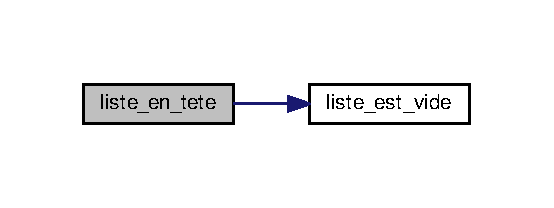
\includegraphics[width=266pt]{liste_8h_a9cbc13cd82829b3541fae0c01209f963_cgraph}
\end{center}
\end{figure}




Here is the caller graph for this function\-:
\nopagebreak
\begin{figure}[H]
\begin{center}
\leavevmode
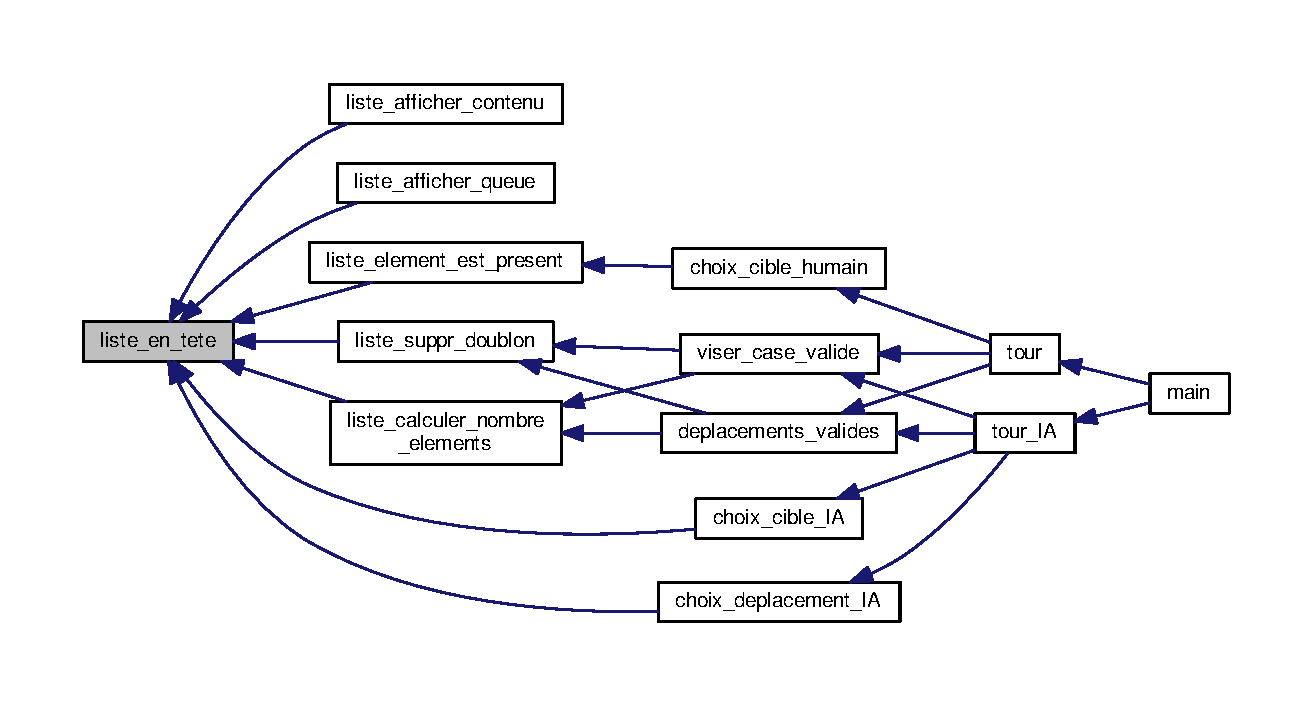
\includegraphics[width=350pt]{liste_8h_a9cbc13cd82829b3541fae0c01209f963_icgraph}
\end{center}
\end{figure}


\hypertarget{liste_8h_ad4a1a49d8756b972708e0870f9420776}{\index{liste.\-h@{liste.\-h}!liste\-\_\-est\-\_\-hors\-\_\-liste@{liste\-\_\-est\-\_\-hors\-\_\-liste}}
\index{liste\-\_\-est\-\_\-hors\-\_\-liste@{liste\-\_\-est\-\_\-hors\-\_\-liste}!liste.h@{liste.\-h}}
\subsubsection[{liste\-\_\-est\-\_\-hors\-\_\-liste}]{\setlength{\rightskip}{0pt plus 5cm}int liste\-\_\-est\-\_\-hors\-\_\-liste (
\begin{DoxyParamCaption}
\item[{void}]{}
\end{DoxyParamCaption}
)}}\label{liste_8h_ad4a1a49d8756b972708e0870f9420776}


Definition at line 25 of file liste.\-c.



Here is the caller graph for this function\-:
\nopagebreak
\begin{figure}[H]
\begin{center}
\leavevmode
\includegraphics[width=350pt]{liste_8h_ad4a1a49d8756b972708e0870f9420776_icgraph}
\end{center}
\end{figure}


\hypertarget{liste_8h_a1e4d1c45ace210278d08fd886268a0e3}{\index{liste.\-h@{liste.\-h}!liste\-\_\-est\-\_\-vide@{liste\-\_\-est\-\_\-vide}}
\index{liste\-\_\-est\-\_\-vide@{liste\-\_\-est\-\_\-vide}!liste.h@{liste.\-h}}
\subsubsection[{liste\-\_\-est\-\_\-vide}]{\setlength{\rightskip}{0pt plus 5cm}int liste\-\_\-est\-\_\-vide (
\begin{DoxyParamCaption}
\item[{void}]{}
\end{DoxyParamCaption}
)}}\label{liste_8h_a1e4d1c45ace210278d08fd886268a0e3}


Definition at line 19 of file liste.\-c.



Here is the caller graph for this function\-:
\nopagebreak
\begin{figure}[H]
\begin{center}
\leavevmode
\includegraphics[width=350pt]{liste_8h_a1e4d1c45ace210278d08fd886268a0e3_icgraph}
\end{center}
\end{figure}


\hypertarget{liste_8h_a522697519e93e19d07943667b472a5c1}{\index{liste.\-h@{liste.\-h}!liste\-\_\-init@{liste\-\_\-init}}
\index{liste\-\_\-init@{liste\-\_\-init}!liste.h@{liste.\-h}}
\subsubsection[{liste\-\_\-init}]{\setlength{\rightskip}{0pt plus 5cm}$<$$<$$<$$<$$<$$<$$<$H\-E\-A\-D=======$>$$>$$>$$>$$>$$>$ void liste\-\_\-init (
\begin{DoxyParamCaption}
\item[{void}]{}
\end{DoxyParamCaption}
)}}\label{liste_8h_a522697519e93e19d07943667b472a5c1}


Definition at line 12 of file liste.\-c.



Here is the caller graph for this function\-:
\nopagebreak
\begin{figure}[H]
\begin{center}
\leavevmode
\includegraphics[width=350pt]{liste_8h_a522697519e93e19d07943667b472a5c1_icgraph}
\end{center}
\end{figure}


\hypertarget{liste_8h_a0282305b4b91dc5376333ac820bdf995}{\index{liste.\-h@{liste.\-h}!liste\-\_\-modif\-\_\-elt@{liste\-\_\-modif\-\_\-elt}}
\index{liste\-\_\-modif\-\_\-elt@{liste\-\_\-modif\-\_\-elt}!liste.h@{liste.\-h}}
\subsubsection[{liste\-\_\-modif\-\_\-elt}]{\setlength{\rightskip}{0pt plus 5cm}void liste\-\_\-modif\-\_\-elt (
\begin{DoxyParamCaption}
\item[{{\bf t\-\_\-coord}}]{v}
\end{DoxyParamCaption}
)}}\label{liste_8h_a0282305b4b91dc5376333ac820bdf995}


Definition at line 66 of file liste.\-c.



Here is the call graph for this function\-:
\nopagebreak
\begin{figure}[H]
\begin{center}
\leavevmode
\includegraphics[width=298pt]{liste_8h_a0282305b4b91dc5376333ac820bdf995_cgraph}
\end{center}
\end{figure}


\hypertarget{liste_8h_ac46b950926c8191e47c3822c624d2e1d}{\index{liste.\-h@{liste.\-h}!liste\-\_\-oter\-\_\-elt@{liste\-\_\-oter\-\_\-elt}}
\index{liste\-\_\-oter\-\_\-elt@{liste\-\_\-oter\-\_\-elt}!liste.h@{liste.\-h}}
\subsubsection[{liste\-\_\-oter\-\_\-elt}]{\setlength{\rightskip}{0pt plus 5cm}void liste\-\_\-oter\-\_\-elt (
\begin{DoxyParamCaption}
\item[{void}]{}
\end{DoxyParamCaption}
)}}\label{liste_8h_ac46b950926c8191e47c3822c624d2e1d}


Definition at line 73 of file liste.\-c.



Here is the call graph for this function\-:
\nopagebreak
\begin{figure}[H]
\begin{center}
\leavevmode
\includegraphics[width=290pt]{liste_8h_ac46b950926c8191e47c3822c624d2e1d_cgraph}
\end{center}
\end{figure}




Here is the caller graph for this function\-:
\nopagebreak
\begin{figure}[H]
\begin{center}
\leavevmode
\includegraphics[width=350pt]{liste_8h_ac46b950926c8191e47c3822c624d2e1d_icgraph}
\end{center}
\end{figure}


\hypertarget{liste_8h_ae62f982aac8059018f004e3a7e2e7f21}{\index{liste.\-h@{liste.\-h}!liste\-\_\-precedent@{liste\-\_\-precedent}}
\index{liste\-\_\-precedent@{liste\-\_\-precedent}!liste.h@{liste.\-h}}
\subsubsection[{liste\-\_\-precedent}]{\setlength{\rightskip}{0pt plus 5cm}void liste\-\_\-precedent (
\begin{DoxyParamCaption}
\item[{void}]{}
\end{DoxyParamCaption}
)}}\label{liste_8h_ae62f982aac8059018f004e3a7e2e7f21}


Definition at line 45 of file liste.\-c.



Here is the call graph for this function\-:
\nopagebreak
\begin{figure}[H]
\begin{center}
\leavevmode
\includegraphics[width=302pt]{liste_8h_ae62f982aac8059018f004e3a7e2e7f21_cgraph}
\end{center}
\end{figure}


\hypertarget{liste_8h_a801cf7ec08fb2c6b1dceb32af4a46111}{\index{liste.\-h@{liste.\-h}!liste\-\_\-suivant@{liste\-\_\-suivant}}
\index{liste\-\_\-suivant@{liste\-\_\-suivant}!liste.h@{liste.\-h}}
\subsubsection[{liste\-\_\-suivant}]{\setlength{\rightskip}{0pt plus 5cm}void liste\-\_\-suivant (
\begin{DoxyParamCaption}
\item[{void}]{}
\end{DoxyParamCaption}
)}}\label{liste_8h_a801cf7ec08fb2c6b1dceb32af4a46111}


Definition at line 52 of file liste.\-c.



Here is the call graph for this function\-:
\nopagebreak
\begin{figure}[H]
\begin{center}
\leavevmode
\includegraphics[width=290pt]{liste_8h_a801cf7ec08fb2c6b1dceb32af4a46111_cgraph}
\end{center}
\end{figure}




Here is the caller graph for this function\-:
\nopagebreak
\begin{figure}[H]
\begin{center}
\leavevmode
\includegraphics[width=350pt]{liste_8h_a801cf7ec08fb2c6b1dceb32af4a46111_icgraph}
\end{center}
\end{figure}


\hypertarget{liste_8h_a48218f7c1bafab1e92490a0963ee7451}{\index{liste.\-h@{liste.\-h}!liste\-\_\-suppr\-\_\-doublon@{liste\-\_\-suppr\-\_\-doublon}}
\index{liste\-\_\-suppr\-\_\-doublon@{liste\-\_\-suppr\-\_\-doublon}!liste.h@{liste.\-h}}
\subsubsection[{liste\-\_\-suppr\-\_\-doublon}]{\setlength{\rightskip}{0pt plus 5cm}void liste\-\_\-suppr\-\_\-doublon (
\begin{DoxyParamCaption}
{}
\end{DoxyParamCaption}
)}}\label{liste_8h_a48218f7c1bafab1e92490a0963ee7451}


Definition at line 143 of file liste.\-c.



Here is the call graph for this function\-:
\nopagebreak
\begin{figure}[H]
\begin{center}
\leavevmode
\includegraphics[width=350pt]{liste_8h_a48218f7c1bafab1e92490a0963ee7451_cgraph}
\end{center}
\end{figure}




Here is the caller graph for this function\-:
\nopagebreak
\begin{figure}[H]
\begin{center}
\leavevmode
\includegraphics[width=350pt]{liste_8h_a48218f7c1bafab1e92490a0963ee7451_icgraph}
\end{center}
\end{figure}


\hypertarget{liste_8h_a1ad09d74d2d4f3b298db6b834933d744}{\index{liste.\-h@{liste.\-h}!liste\-\_\-valeur\-\_\-elt@{liste\-\_\-valeur\-\_\-elt}}
\index{liste\-\_\-valeur\-\_\-elt@{liste\-\_\-valeur\-\_\-elt}!liste.h@{liste.\-h}}
\subsubsection[{liste\-\_\-valeur\-\_\-elt}]{\setlength{\rightskip}{0pt plus 5cm}void liste\-\_\-valeur\-\_\-elt (
\begin{DoxyParamCaption}
\item[{{\bf t\-\_\-coord} $\ast$}]{e}
\end{DoxyParamCaption}
)}}\label{liste_8h_a1ad09d74d2d4f3b298db6b834933d744}


Definition at line 59 of file liste.\-c.



Here is the call graph for this function\-:
\nopagebreak
\begin{figure}[H]
\begin{center}
\leavevmode
\includegraphics[width=300pt]{liste_8h_a1ad09d74d2d4f3b298db6b834933d744_cgraph}
\end{center}
\end{figure}




Here is the caller graph for this function\-:
\nopagebreak
\begin{figure}[H]
\begin{center}
\leavevmode
\includegraphics[width=350pt]{liste_8h_a1ad09d74d2d4f3b298db6b834933d744_icgraph}
\end{center}
\end{figure}



\hypertarget{_minimale_8c}{\section{Référence du fichier Minimale.\-c}
\label{_minimale_8c}\index{Minimale.\-c@{Minimale.\-c}}
}
{\ttfamily \#include $<$assert.\-h$>$}\\*
{\ttfamily \#include $<$stdlib.\-h$>$}\\*
{\ttfamily \#include $<$stdio.\-h$>$}\\*
{\ttfamily \#include $<$string.\-h$>$}\\*
{\ttfamily \#include $<$time.\-h$>$}\\*
{\ttfamily \#include $<$ctype.\-h$>$}\\*
{\ttfamily \#include $<$ncurses.\-h$>$}\\*
{\ttfamily \#include \char`\"{}header.\-h\char`\"{}}\\*
{\ttfamily \#include \char`\"{}liste.\-h\char`\"{}}\\*
{\ttfamily \#include \char`\"{}file.\-h\char`\"{}}\\*
{\ttfamily \#include \char`\"{}pile.\-h\char`\"{}}\\*
Graphe des dépendances par inclusion de Minimale.\-c\-:\nopagebreak
\begin{figure}[H]
\begin{center}
\leavevmode
\includegraphics[width=350pt]{_minimale_8c__incl}
\end{center}
\end{figure}
\subsection*{Macros}
\begin{DoxyCompactItemize}
\item 
\#define \hyperlink{_minimale_8c_a137aa83ec74421d226a90c92ec032ac9}{K\-N\-R\-M}~\char`\"{}\textbackslash{}x1\-B\mbox{[}0m\char`\"{}
\item 
\#define \hyperlink{_minimale_8c_a66290957baed5df3930ada4cb8caccf1}{K\-R\-E\-D}~\char`\"{}\textbackslash{}x1\-B\mbox{[}31m\char`\"{}
\item 
\#define \hyperlink{_minimale_8c_ac081c83b067273757f7a2e54a5957d41}{K\-G\-R\-N}~\char`\"{}\textbackslash{}x1\-B\mbox{[}32m\char`\"{}
\item 
\#define \hyperlink{_minimale_8c_a897b10d246533c95ba86cb79f92e465a}{K\-Y\-E\-L}~\char`\"{}\textbackslash{}x1\-B\mbox{[}33m\char`\"{}
\item 
\#define \hyperlink{_minimale_8c_a3f838f2fc3a9a3b434be606fc908964b}{K\-B\-L\-U}~\char`\"{}\textbackslash{}x1\-B\mbox{[}34m\char`\"{}
\item 
\#define \hyperlink{_minimale_8c_a6825f05d3b9d619d91d79d0ef18bb8b2}{K\-M\-A\-G}~\char`\"{}\textbackslash{}x1\-B\mbox{[}35m\char`\"{}
\item 
\#define \hyperlink{_minimale_8c_a32036c94dbb166a3f874b7efc169841f}{K\-C\-Y\-N}~\char`\"{}\textbackslash{}x1\-B\mbox{[}36m\char`\"{}
\item 
\#define \hyperlink{_minimale_8c_af0036c8022c9980079ab17e5c87fd478}{K\-W\-H\-T}~\char`\"{}\textbackslash{}x1\-B\mbox{[}37m\char`\"{}
\end{DoxyCompactItemize}
\subsection*{Fonctions}
\begin{DoxyCompactItemize}
\item 
int \hyperlink{_minimale_8c_a704aac80f0e314dab07203a35f05aef2}{life\-\_\-check} (int joueur\-\_\-courant)
\begin{DoxyCompactList}\small\item\em Fonction qui vérifie si un joueur a encore des personnages vivants sur le terrain. Appelle \hyperlink{_minimale_8c_ae1d5aa28a687b31b055f49ea44866780}{are\-\_\-my\-\_\-mates\-\_\-alive(int joueur\-\_\-courant)} pour déterminer le joueur est encore en jeu. Renvoie 1 si le joueur a encore des personnages en vie, sinon 0. \end{DoxyCompactList}\item 
void \hyperlink{_minimale_8c_a1f36ed2102ea6a97801ef419173a730b}{joueur\-\_\-liste\-\_\-suivant} (int nb\-\_\-joueur, int $\ast$joueur\-\_\-courant)
\begin{DoxyCompactList}\small\item\em Prend en paramètre le nombre de joueurs et incrémente le numéro de joueur de façon à ne pas dépasser le nombre de joueurs. \end{DoxyCompactList}\item 
void \hyperlink{_minimale_8c_a88cec99ca1b112fc0553d0f09c19fcd7}{creer\-\_\-terrain\-\_\-rapide} (\hyperlink{header_8h_a4bb25c9352f7bb2ea2eb663ccf579528}{t\-\_\-camp} camp, int x, int y)
\begin{DoxyCompactList}\small\item\em Création brève de terrain ou obstacle, possible implémentation de génération aléatoire en cas d'obstacle. \end{DoxyCompactList}\item 
void \hyperlink{_minimale_8c_a183c5f911befa83432ff61674e326603}{vider\-\_\-buffer} (void)
\begin{DoxyCompactList}\small\item\em Vide le tampon de saisie clavier. \end{DoxyCompactList}\item 
int \hyperlink{_minimale_8c_ae1d5aa28a687b31b055f49ea44866780}{are\-\_\-my\-\_\-mates\-\_\-alive} (int joueur\-\_\-courant)
\item 
int \hyperlink{_minimale_8c_a0255b1b3f70d1d35a858e9e512c8f988}{calcul\-\_\-persos\-\_\-\-I\-A} (int joueur\-\_\-courant)
\item 
void \hyperlink{_minimale_8c_a1fdf262e6e18d594322ddcfdde4e4b3e}{afficher\-\_\-plateau\-\_\-orientation} (int joueur\-\_\-courant)
\begin{DoxyCompactList}\small\item\em Affiche le plateau avec les caractères correspondants à l'orientation. \end{DoxyCompactList}\item 
void \hyperlink{_minimale_8c_a97c357428c810b5f8ed3fcbeb973dd88}{generation\-\_\-nom\-\_\-personnage} (char $\ast$nom)
\item 
void \hyperlink{_minimale_8c_a01e6e73a74f481fc32b060f3e52b8a5f}{players\-\_\-life\-\_\-check} ()
\begin{DoxyCompactList}\small\item\em Actualise le fait que les joueurs soient vivants ou non. \end{DoxyCompactList}\item 
void \hyperlink{_minimale_8c_aebdcead4bd058408b30ee5924910d1f6}{Sauvegarder} (int joueur\-\_\-courant)
\item 
void \hyperlink{_minimale_8c_a49285114d9ea55b17aaaf5b5e21432a5}{Charger} (int joueur\-\_\-courant)
\item 
int \hyperlink{_minimale_8c_a693e68e5f8ca09f46ad6b746c07d0332}{generation\-\_\-nombre\-\_\-aleatoire} (int max)
\begin{DoxyCompactList}\small\item\em Fonction qui renvoi un nombre aléatoire en 0 et 'max'. \end{DoxyCompactList}\item 
void \hyperlink{_minimale_8c_a3f74d85bb951bc6b755696903c848531}{deplacer\-\_\-perso} (\hyperlink{structt__coord}{t\-\_\-coord} case\-\_\-perso)
\begin{DoxyCompactList}\small\item\em Déplace le personnage sur le terrain. \end{DoxyCompactList}\item 
int \hyperlink{_minimale_8c_ac07dd1dbd17abd8de085e601421c8103}{cases\-\_\-voisines\-\_\-calcul} (\hyperlink{structt__coord}{t\-\_\-coord} coordonnees)
\begin{DoxyCompactList}\small\item\em Renvoi le nombre de case voisine vide, met dans la file la liste des coordonnées voisines accessibles. \end{DoxyCompactList}\item 
void \hyperlink{_minimale_8c_aaadb3730c96b5ae1d0fc498c3432f6a5}{deplacements\-\_\-valides} (int $\ast$nb\-Dep\-Valid)
\begin{DoxyCompactList}\small\item\em Calcule les positions de déplacement valide, les met dans la liste. \end{DoxyCompactList}\item 
\hyperlink{structt__coord}{t\-\_\-coord} \hyperlink{_minimale_8c_a22abc2bad1fd63372797a0e3fe103f07}{choix\-\_\-deplacement\-\_\-humain} (int joueur\-\_\-courant, int $\ast$nb\-Dep\-Valid)
\item 
\hyperlink{structt__coord}{t\-\_\-coord} \hyperlink{_minimale_8c_aa1c28f345f10a0f18458c5aa14e73c79}{choix\-\_\-deplacement\-\_\-\-I\-A} (int $\ast$nb\-Dep\-Valid)
\item 
void \hyperlink{_minimale_8c_aa17c4e2a8512aa83516a20e0df29a123}{init\-\_\-plateau} ()
\begin{DoxyCompactList}\small\item\em Initialise le plateau en le remplissant de terrain par défaut. \end{DoxyCompactList}\item 
int \hyperlink{_minimale_8c_ad6b417d8f6547affac1cc287a6762113}{cases\-\_\-voisines\-\_\-\-A\-T\-K} (\hyperlink{structt__coord}{t\-\_\-coord} coordonnees)
\item 
void \hyperlink{_minimale_8c_a93abf905224d72b20101bb2a6e0ab417}{viser\-\_\-case\-\_\-valide} (\hyperlink{structt__skill}{t\-\_\-skill} skill, int $\ast$nb\-Atk\-Valid)
\item 
\hyperlink{structt__coord}{t\-\_\-coord} \hyperlink{_minimale_8c_a29cde2a1505f65c5b2b190588516f6d6}{choix\-\_\-cible\-\_\-\-I\-A} (\hyperlink{structt__skill}{t\-\_\-skill} skill, int $\ast$nb\-Atk\-Valid)
\item 
void \hyperlink{_minimale_8c_ad7419c3036235a80b59bc983660be2ee}{init\-\_\-char\-\_\-table} (\hyperlink{structt__character}{t\-\_\-character} chars\mbox{[}$\,$\mbox{]})
\item 
void \hyperlink{_minimale_8c_af5c4cbfb002da8b8595316d87548ab93}{afficher\-\_\-skill} (int skill\-\_\-nb, \hyperlink{structt__skill}{t\-\_\-skill} skill)
\item 
void \hyperlink{_minimale_8c_a7015d7153fc65e628d81cdd3b68ab7ec}{afficher\-\_\-skill\-\_\-list} (\hyperlink{structt__character}{t\-\_\-character} perso)
\item 
void \hyperlink{_minimale_8c_ad312ec60fc8d45f956471549de9ab21c}{afficher\-\_\-infos\-\_\-persos} (\hyperlink{structt__character}{t\-\_\-character} perso)
\item 
\hyperlink{structt__coord}{t\-\_\-coord} \hyperlink{_minimale_8c_a7c9c98d472a87c9f8a877ceb74dea5ac}{choix\-\_\-cible\-\_\-humain} (\hyperlink{structt__skill}{t\-\_\-skill} skill, int joueur\-\_\-courant)
\item 
void \hyperlink{_minimale_8c_ae7570939d9a77836280496452e995a49}{selection\-\_\-perso} (int joueur\-\_\-courant)
\begin{DoxyCompactList}\small\item\em Fonction qui propose la liste des personnages pouvant être sélectionnés. \end{DoxyCompactList}\item 
void \hyperlink{_minimale_8c_add579b3bffa443553769bdacdd18a9e0}{passer\-\_\-tour} ()
\begin{DoxyCompactList}\small\item\em Fonction qui passe le tour du joueur actif. \end{DoxyCompactList}\item 
void \hyperlink{_minimale_8c_af96504b67683769d99d267ab8244cdc8}{suicide} (int joueur\-\_\-courant)
\begin{DoxyCompactList}\small\item\em Fonction permetant au joueur courant d'abandonner la partie. \end{DoxyCompactList}\item 
\hyperlink{structt__skill}{t\-\_\-skill} \hyperlink{_minimale_8c_a10f645fb2dcd1253cf4b728d7020b727}{select\-\_\-skill\-\_\-\-I\-A} ()
\item 
\hyperlink{structt__skill}{t\-\_\-skill} \hyperlink{_minimale_8c_a54b8579a2cf79307a0ce11d29597d2f1}{select\-\_\-skill} ()
\item 
\hyperlink{header_8h_a05b909310980a637d41bd67fc4d5c389}{t\-\_\-target\-Orientation} \hyperlink{_minimale_8c_a32d1e9030c1705ad183484acce8a4b2c}{get\-\_\-target\-\_\-orientation} (\hyperlink{structt__character}{t\-\_\-character} perso, \hyperlink{structt__coord}{t\-\_\-coord} cible)
\begin{DoxyCompactList}\small\item\em Fonction déterminant quelle est l'orientation de la cible par rapport au joueur. \end{DoxyCompactList}\item 
void \hyperlink{_minimale_8c_a28d9c8c6a5abddd6a89ddb258b5114bc}{appliquer\-\_\-action} (\hyperlink{structt__character}{t\-\_\-character} lanceur, \hyperlink{structt__coord}{t\-\_\-coord} cible, \hyperlink{structt__skill}{t\-\_\-skill} action)
\begin{DoxyCompactList}\small\item\em Fonction appliquant le skill du personnage lanceur à la case cible. Remplit le tableau de personnages entré en paramètre de cases de terrain. \end{DoxyCompactList}\item 
void \hyperlink{_minimale_8c_a2ee0cc6d76b7e497988562a817c096a1}{orienter\-\_\-perso\-\_\-numpad} (int joueur\-\_\-courant)
\begin{DoxyCompactList}\small\item\em Propose une liste numérique des orientations du perso indiqué en paramètre d'entrée et change son orientation. \end{DoxyCompactList}\item 
void \hyperlink{_minimale_8c_ae628b0fb007cb8d89fe76de11151934e}{orienter\-\_\-perso} ()
\item 
int \hyperlink{_minimale_8c_a0529503b2d07980eab95dcd282587007}{perso\-\_\-oriente\-\_\-a\-\_\-droite} ()
\item 
void \hyperlink{_minimale_8c_a21af16606028cc5f140a51a2314c2668}{character\-\_\-hp\-\_\-list} ()
\begin{DoxyCompactList}\small\item\em affiche une liste avec les persos et leurs points de vie. \end{DoxyCompactList}\item 
void \hyperlink{_minimale_8c_a779ee1563d913e90d9ad93b9adf6867e}{tour} (int joueur\-\_\-courant, int $\ast$nb\-Atk\-Valid, int $\ast$nb\-Dep\-Valid)
\item 
int \hyperlink{_minimale_8c_aa6bc2b819d20d08ea1c98f09c15f2c47}{all\-\_\-dead\-\_\-but\-\_\-one} (int nb\-\_\-joueurs)
\item 
void \hyperlink{_minimale_8c_afbbdb6480cb3ab0ba8f8ac1615d4e22e}{creer\-\_\-perso\-\_\-rapide} (\hyperlink{header_8h_a4bb25c9352f7bb2ea2eb663ccf579528}{t\-\_\-camp} camp, int x, int y)
\item 
void \hyperlink{_minimale_8c_af63ad36c60d60f979a15f7bf3a24c5a3}{edit\-\_\-stats} (\hyperlink{structt__character}{t\-\_\-character} perso, int H\-P, int Max\-\_\-\-H\-P, int M\-P, int Max\-\_\-\-M\-P, int \hyperlink{header_8h_a440f669d36bc2028077af38574051204a52c6d49f971f8f70cf3f3c474edc08f9}{A\-T\-K}, int \hyperlink{header_8h_a440f669d36bc2028077af38574051204a1fe261f2a80ef9b7055433a3c2d93af8}{M\-A\-T\-K}, int D\-E\-F, int M\-D\-E\-F, int M\-V\-T)
\item 
void \hyperlink{_minimale_8c_ae5778c7cb58f5d0dc868b2c3f632574e}{spawn\-\_\-sauvage} ()
\item 
void \hyperlink{_minimale_8c_a670d6c4a5f077fec01afb7b253ddc320}{spawn\-\_\-character} (\hyperlink{header_8h_a4bb25c9352f7bb2ea2eb663ccf579528}{t\-\_\-camp} camp\-\_\-nouveau\-\_\-perso)
\item 
void \hyperlink{_minimale_8c_aee3a984cc380669ef226b08039d592da}{tour\-\_\-\-I\-A} (int joueur\-\_\-courant, int $\ast$nb\-Atk\-Valid, int $\ast$nb\-Dep\-Valid)
\item 
void \hyperlink{_minimale_8c_a0b7596f8f2c018a80e51c70268d338fd}{saisie\-\_\-nombre\-\_\-joueurs} (int $\ast$nb\-\_\-joueurs)
\item 
int \hyperlink{_minimale_8c_ae66f6b31b5ad750f1fe042a706a4e3d4}{main} ()
\begin{DoxyCompactList}\small\item\em Fonction principale Fonction principale qui permet de jouer en mode Kill'em'all. \end{DoxyCompactList}\end{DoxyCompactItemize}
\subsection*{Variables}
\begin{DoxyCompactItemize}
\item 
int \hyperlink{_minimale_8c_a66ecc67604b45591ca621e1c1936d009}{compteur\-\_\-tour} =0
\item 
int \hyperlink{_minimale_8c_aeb67ecf1ba206af9765bba7ecd7cd929}{compteur\-\_\-joueurs\-\_\-vivants} =0
\item 
\hyperlink{structt__character}{t\-\_\-character} \hyperlink{_minimale_8c_a0d10b4d51713595a0aecf92594403ca3}{Valid\-\_\-chars\-\_\-\-I\-A} \mbox{[}\hyperlink{header_8h_a220380eaa4bfe0ffeab9859c6f3d2076}{Max\-Tab}\mbox{]}
\item 
char \hyperlink{_minimale_8c_a08b1b223d56118ff55a1caf616e22186}{particule\-\_\-generateur\-\_\-nom} \mbox{[}$\,$\mbox{]}\mbox{[}20\mbox{]}
\item 
\hyperlink{structt__character}{t\-\_\-character} \hyperlink{_minimale_8c_afd49c2feefa9ee6ce4af9beea5b8a88c}{selected\-\_\-character}
\item 
\hyperlink{structt__character}{t\-\_\-character} \hyperlink{_minimale_8c_a816e050bd234e1024a41068177f1ac49}{Plateau} \mbox{[}\hyperlink{header_8h_a523c276fa2df3dd24764b5bb500dbde6}{T\-A\-I\-L\-L\-E\-\_\-\-M\-A\-T\-R\-I\-C\-E}\mbox{]}\mbox{[}\hyperlink{header_8h_a523c276fa2df3dd24764b5bb500dbde6}{T\-A\-I\-L\-L\-E\-\_\-\-M\-A\-T\-R\-I\-C\-E}\mbox{]}
\item 
\hyperlink{structt__coord}{t\-\_\-coord} \hyperlink{_minimale_8c_a5a6e59130d22bce1f5ec9490b20d7fb3}{dep\-Valid} \mbox{[}\hyperlink{header_8h_a523c276fa2df3dd24764b5bb500dbde6}{T\-A\-I\-L\-L\-E\-\_\-\-M\-A\-T\-R\-I\-C\-E} $\ast$\hyperlink{header_8h_a523c276fa2df3dd24764b5bb500dbde6}{T\-A\-I\-L\-L\-E\-\_\-\-M\-A\-T\-R\-I\-C\-E}\mbox{]}\mbox{[}3\mbox{]}
\item 
\hyperlink{structt__player}{t\-\_\-player} \hyperlink{_minimale_8c_adb6f8f74ea8aeb8c5a3f0d838ca80999}{player} \mbox{[}\hyperlink{header_8h_a220380eaa4bfe0ffeab9859c6f3d2076}{Max\-Tab}\mbox{]}
\item 
int \hyperlink{_minimale_8c_a6cfe6e5ba882446145a8c3f5508e2ea6}{indice\-Tab\-Dep\-Valid}
\end{DoxyCompactItemize}


\subsection{Documentation des macros}
\hypertarget{_minimale_8c_a3f838f2fc3a9a3b434be606fc908964b}{\index{Minimale.\-c@{Minimale.\-c}!K\-B\-L\-U@{K\-B\-L\-U}}
\index{K\-B\-L\-U@{K\-B\-L\-U}!Minimale.c@{Minimale.\-c}}
\subsubsection[{K\-B\-L\-U}]{\setlength{\rightskip}{0pt plus 5cm}\#define K\-B\-L\-U~\char`\"{}\textbackslash{}x1\-B\mbox{[}34m\char`\"{}}}\label{_minimale_8c_a3f838f2fc3a9a3b434be606fc908964b}


Définition à la ligne 20 du fichier Minimale.\-c.

\hypertarget{_minimale_8c_a32036c94dbb166a3f874b7efc169841f}{\index{Minimale.\-c@{Minimale.\-c}!K\-C\-Y\-N@{K\-C\-Y\-N}}
\index{K\-C\-Y\-N@{K\-C\-Y\-N}!Minimale.c@{Minimale.\-c}}
\subsubsection[{K\-C\-Y\-N}]{\setlength{\rightskip}{0pt plus 5cm}\#define K\-C\-Y\-N~\char`\"{}\textbackslash{}x1\-B\mbox{[}36m\char`\"{}}}\label{_minimale_8c_a32036c94dbb166a3f874b7efc169841f}


Définition à la ligne 22 du fichier Minimale.\-c.

\hypertarget{_minimale_8c_ac081c83b067273757f7a2e54a5957d41}{\index{Minimale.\-c@{Minimale.\-c}!K\-G\-R\-N@{K\-G\-R\-N}}
\index{K\-G\-R\-N@{K\-G\-R\-N}!Minimale.c@{Minimale.\-c}}
\subsubsection[{K\-G\-R\-N}]{\setlength{\rightskip}{0pt plus 5cm}\#define K\-G\-R\-N~\char`\"{}\textbackslash{}x1\-B\mbox{[}32m\char`\"{}}}\label{_minimale_8c_ac081c83b067273757f7a2e54a5957d41}


Définition à la ligne 18 du fichier Minimale.\-c.

\hypertarget{_minimale_8c_a6825f05d3b9d619d91d79d0ef18bb8b2}{\index{Minimale.\-c@{Minimale.\-c}!K\-M\-A\-G@{K\-M\-A\-G}}
\index{K\-M\-A\-G@{K\-M\-A\-G}!Minimale.c@{Minimale.\-c}}
\subsubsection[{K\-M\-A\-G}]{\setlength{\rightskip}{0pt plus 5cm}\#define K\-M\-A\-G~\char`\"{}\textbackslash{}x1\-B\mbox{[}35m\char`\"{}}}\label{_minimale_8c_a6825f05d3b9d619d91d79d0ef18bb8b2}


Définition à la ligne 21 du fichier Minimale.\-c.

\hypertarget{_minimale_8c_a137aa83ec74421d226a90c92ec032ac9}{\index{Minimale.\-c@{Minimale.\-c}!K\-N\-R\-M@{K\-N\-R\-M}}
\index{K\-N\-R\-M@{K\-N\-R\-M}!Minimale.c@{Minimale.\-c}}
\subsubsection[{K\-N\-R\-M}]{\setlength{\rightskip}{0pt plus 5cm}\#define K\-N\-R\-M~\char`\"{}\textbackslash{}x1\-B\mbox{[}0m\char`\"{}}}\label{_minimale_8c_a137aa83ec74421d226a90c92ec032ac9}


Définition à la ligne 16 du fichier Minimale.\-c.

\hypertarget{_minimale_8c_a66290957baed5df3930ada4cb8caccf1}{\index{Minimale.\-c@{Minimale.\-c}!K\-R\-E\-D@{K\-R\-E\-D}}
\index{K\-R\-E\-D@{K\-R\-E\-D}!Minimale.c@{Minimale.\-c}}
\subsubsection[{K\-R\-E\-D}]{\setlength{\rightskip}{0pt plus 5cm}\#define K\-R\-E\-D~\char`\"{}\textbackslash{}x1\-B\mbox{[}31m\char`\"{}}}\label{_minimale_8c_a66290957baed5df3930ada4cb8caccf1}


Définition à la ligne 17 du fichier Minimale.\-c.

\hypertarget{_minimale_8c_af0036c8022c9980079ab17e5c87fd478}{\index{Minimale.\-c@{Minimale.\-c}!K\-W\-H\-T@{K\-W\-H\-T}}
\index{K\-W\-H\-T@{K\-W\-H\-T}!Minimale.c@{Minimale.\-c}}
\subsubsection[{K\-W\-H\-T}]{\setlength{\rightskip}{0pt plus 5cm}\#define K\-W\-H\-T~\char`\"{}\textbackslash{}x1\-B\mbox{[}37m\char`\"{}}}\label{_minimale_8c_af0036c8022c9980079ab17e5c87fd478}


Définition à la ligne 23 du fichier Minimale.\-c.

\hypertarget{_minimale_8c_a897b10d246533c95ba86cb79f92e465a}{\index{Minimale.\-c@{Minimale.\-c}!K\-Y\-E\-L@{K\-Y\-E\-L}}
\index{K\-Y\-E\-L@{K\-Y\-E\-L}!Minimale.c@{Minimale.\-c}}
\subsubsection[{K\-Y\-E\-L}]{\setlength{\rightskip}{0pt plus 5cm}\#define K\-Y\-E\-L~\char`\"{}\textbackslash{}x1\-B\mbox{[}33m\char`\"{}}}\label{_minimale_8c_a897b10d246533c95ba86cb79f92e465a}


Définition à la ligne 19 du fichier Minimale.\-c.



\subsection{Documentation des fonctions}
\hypertarget{_minimale_8c_ad312ec60fc8d45f956471549de9ab21c}{\index{Minimale.\-c@{Minimale.\-c}!afficher\-\_\-infos\-\_\-persos@{afficher\-\_\-infos\-\_\-persos}}
\index{afficher\-\_\-infos\-\_\-persos@{afficher\-\_\-infos\-\_\-persos}!Minimale.c@{Minimale.\-c}}
\subsubsection[{afficher\-\_\-infos\-\_\-persos}]{\setlength{\rightskip}{0pt plus 5cm}void afficher\-\_\-infos\-\_\-persos (
\begin{DoxyParamCaption}
\item[{{\bf t\-\_\-character}}]{perso}
\end{DoxyParamCaption}
)}}\label{_minimale_8c_ad312ec60fc8d45f956471549de9ab21c}


Définition à la ligne 651 du fichier Minimale.\-c.



Voici le graphe d'appel pour cette fonction \-:\nopagebreak
\begin{figure}[H]
\begin{center}
\leavevmode
\includegraphics[width=350pt]{_minimale_8c_ad312ec60fc8d45f956471549de9ab21c_cgraph}
\end{center}
\end{figure}




Voici le graphe des appelants de cette fonction \-:\nopagebreak
\begin{figure}[H]
\begin{center}
\leavevmode
\includegraphics[width=350pt]{_minimale_8c_ad312ec60fc8d45f956471549de9ab21c_icgraph}
\end{center}
\end{figure}


\hypertarget{_minimale_8c_a1fdf262e6e18d594322ddcfdde4e4b3e}{\index{Minimale.\-c@{Minimale.\-c}!afficher\-\_\-plateau\-\_\-orientation@{afficher\-\_\-plateau\-\_\-orientation}}
\index{afficher\-\_\-plateau\-\_\-orientation@{afficher\-\_\-plateau\-\_\-orientation}!Minimale.c@{Minimale.\-c}}
\subsubsection[{afficher\-\_\-plateau\-\_\-orientation}]{\setlength{\rightskip}{0pt plus 5cm}void afficher\-\_\-plateau\-\_\-orientation (
\begin{DoxyParamCaption}
\item[{int}]{joueur\-\_\-courant}
\end{DoxyParamCaption}
)}}\label{_minimale_8c_a1fdf262e6e18d594322ddcfdde4e4b3e}


Affiche le plateau avec les caractères correspondants à l'orientation. 



Définition à la ligne 1548 du fichier Minimale.\-c.



Voici le graphe des appelants de cette fonction \-:\nopagebreak
\begin{figure}[H]
\begin{center}
\leavevmode
\includegraphics[width=350pt]{_minimale_8c_a1fdf262e6e18d594322ddcfdde4e4b3e_icgraph}
\end{center}
\end{figure}


\hypertarget{_minimale_8c_af5c4cbfb002da8b8595316d87548ab93}{\index{Minimale.\-c@{Minimale.\-c}!afficher\-\_\-skill@{afficher\-\_\-skill}}
\index{afficher\-\_\-skill@{afficher\-\_\-skill}!Minimale.c@{Minimale.\-c}}
\subsubsection[{afficher\-\_\-skill}]{\setlength{\rightskip}{0pt plus 5cm}void afficher\-\_\-skill (
\begin{DoxyParamCaption}
\item[{int}]{skill\-\_\-nb, }
\item[{{\bf t\-\_\-skill}}]{skill}
\end{DoxyParamCaption}
)}}\label{_minimale_8c_af5c4cbfb002da8b8595316d87548ab93}


Définition à la ligne 630 du fichier Minimale.\-c.



Voici le graphe des appelants de cette fonction \-:\nopagebreak
\begin{figure}[H]
\begin{center}
\leavevmode
\includegraphics[width=350pt]{_minimale_8c_af5c4cbfb002da8b8595316d87548ab93_icgraph}
\end{center}
\end{figure}


\hypertarget{_minimale_8c_a7015d7153fc65e628d81cdd3b68ab7ec}{\index{Minimale.\-c@{Minimale.\-c}!afficher\-\_\-skill\-\_\-list@{afficher\-\_\-skill\-\_\-list}}
\index{afficher\-\_\-skill\-\_\-list@{afficher\-\_\-skill\-\_\-list}!Minimale.c@{Minimale.\-c}}
\subsubsection[{afficher\-\_\-skill\-\_\-list}]{\setlength{\rightskip}{0pt plus 5cm}void afficher\-\_\-skill\-\_\-list (
\begin{DoxyParamCaption}
\item[{{\bf t\-\_\-character}}]{perso}
\end{DoxyParamCaption}
)}}\label{_minimale_8c_a7015d7153fc65e628d81cdd3b68ab7ec}


Définition à la ligne 642 du fichier Minimale.\-c.



Voici le graphe d'appel pour cette fonction \-:\nopagebreak
\begin{figure}[H]
\begin{center}
\leavevmode
\includegraphics[width=278pt]{_minimale_8c_a7015d7153fc65e628d81cdd3b68ab7ec_cgraph}
\end{center}
\end{figure}




Voici le graphe des appelants de cette fonction \-:\nopagebreak
\begin{figure}[H]
\begin{center}
\leavevmode
\includegraphics[width=350pt]{_minimale_8c_a7015d7153fc65e628d81cdd3b68ab7ec_icgraph}
\end{center}
\end{figure}


\hypertarget{_minimale_8c_aa6bc2b819d20d08ea1c98f09c15f2c47}{\index{Minimale.\-c@{Minimale.\-c}!all\-\_\-dead\-\_\-but\-\_\-one@{all\-\_\-dead\-\_\-but\-\_\-one}}
\index{all\-\_\-dead\-\_\-but\-\_\-one@{all\-\_\-dead\-\_\-but\-\_\-one}!Minimale.c@{Minimale.\-c}}
\subsubsection[{all\-\_\-dead\-\_\-but\-\_\-one}]{\setlength{\rightskip}{0pt plus 5cm}int all\-\_\-dead\-\_\-but\-\_\-one (
\begin{DoxyParamCaption}
\item[{int}]{nb\-\_\-joueurs}
\end{DoxyParamCaption}
)}}\label{_minimale_8c_aa6bc2b819d20d08ea1c98f09c15f2c47}


Définition à la ligne 1530 du fichier Minimale.\-c.



Voici le graphe des appelants de cette fonction \-:\nopagebreak
\begin{figure}[H]
\begin{center}
\leavevmode
\includegraphics[width=246pt]{_minimale_8c_aa6bc2b819d20d08ea1c98f09c15f2c47_icgraph}
\end{center}
\end{figure}


\hypertarget{_minimale_8c_a28d9c8c6a5abddd6a89ddb258b5114bc}{\index{Minimale.\-c@{Minimale.\-c}!appliquer\-\_\-action@{appliquer\-\_\-action}}
\index{appliquer\-\_\-action@{appliquer\-\_\-action}!Minimale.c@{Minimale.\-c}}
\subsubsection[{appliquer\-\_\-action}]{\setlength{\rightskip}{0pt plus 5cm}void appliquer\-\_\-action (
\begin{DoxyParamCaption}
\item[{{\bf t\-\_\-character}}]{lanceur, }
\item[{{\bf t\-\_\-coord}}]{cible, }
\item[{{\bf t\-\_\-skill}}]{action}
\end{DoxyParamCaption}
)}}\label{_minimale_8c_a28d9c8c6a5abddd6a89ddb258b5114bc}


Fonction appliquant le skill du personnage lanceur à la case cible. Remplit le tableau de personnages entré en paramètre de cases de terrain. 



Définition à la ligne 1093 du fichier Minimale.\-c.



Voici le graphe d'appel pour cette fonction \-:\nopagebreak
\begin{figure}[H]
\begin{center}
\leavevmode
\includegraphics[width=314pt]{_minimale_8c_a28d9c8c6a5abddd6a89ddb258b5114bc_cgraph}
\end{center}
\end{figure}




Voici le graphe des appelants de cette fonction \-:\nopagebreak
\begin{figure}[H]
\begin{center}
\leavevmode
\includegraphics[width=326pt]{_minimale_8c_a28d9c8c6a5abddd6a89ddb258b5114bc_icgraph}
\end{center}
\end{figure}


\hypertarget{_minimale_8c_ae1d5aa28a687b31b055f49ea44866780}{\index{Minimale.\-c@{Minimale.\-c}!are\-\_\-my\-\_\-mates\-\_\-alive@{are\-\_\-my\-\_\-mates\-\_\-alive}}
\index{are\-\_\-my\-\_\-mates\-\_\-alive@{are\-\_\-my\-\_\-mates\-\_\-alive}!Minimale.c@{Minimale.\-c}}
\subsubsection[{are\-\_\-my\-\_\-mates\-\_\-alive}]{\setlength{\rightskip}{0pt plus 5cm}int are\-\_\-my\-\_\-mates\-\_\-alive (
\begin{DoxyParamCaption}
\item[{int}]{joueur\-\_\-courant}
\end{DoxyParamCaption}
)}}\label{_minimale_8c_ae1d5aa28a687b31b055f49ea44866780}


Définition à la ligne 1305 du fichier Minimale.\-c.



Voici le graphe des appelants de cette fonction \-:\nopagebreak
\begin{figure}[H]
\begin{center}
\leavevmode
\includegraphics[width=350pt]{_minimale_8c_ae1d5aa28a687b31b055f49ea44866780_icgraph}
\end{center}
\end{figure}


\hypertarget{_minimale_8c_a0255b1b3f70d1d35a858e9e512c8f988}{\index{Minimale.\-c@{Minimale.\-c}!calcul\-\_\-persos\-\_\-\-I\-A@{calcul\-\_\-persos\-\_\-\-I\-A}}
\index{calcul\-\_\-persos\-\_\-\-I\-A@{calcul\-\_\-persos\-\_\-\-I\-A}!Minimale.c@{Minimale.\-c}}
\subsubsection[{calcul\-\_\-persos\-\_\-\-I\-A}]{\setlength{\rightskip}{0pt plus 5cm}int calcul\-\_\-persos\-\_\-\-I\-A (
\begin{DoxyParamCaption}
\item[{int}]{joueur\-\_\-courant}
\end{DoxyParamCaption}
)}}\label{_minimale_8c_a0255b1b3f70d1d35a858e9e512c8f988}


Définition à la ligne 1775 du fichier Minimale.\-c.



Voici le graphe d'appel pour cette fonction \-:\nopagebreak
\begin{figure}[H]
\begin{center}
\leavevmode
\includegraphics[width=288pt]{_minimale_8c_a0255b1b3f70d1d35a858e9e512c8f988_cgraph}
\end{center}
\end{figure}




Voici le graphe des appelants de cette fonction \-:\nopagebreak
\begin{figure}[H]
\begin{center}
\leavevmode
\includegraphics[width=330pt]{_minimale_8c_a0255b1b3f70d1d35a858e9e512c8f988_icgraph}
\end{center}
\end{figure}


\hypertarget{_minimale_8c_ad6b417d8f6547affac1cc287a6762113}{\index{Minimale.\-c@{Minimale.\-c}!cases\-\_\-voisines\-\_\-\-A\-T\-K@{cases\-\_\-voisines\-\_\-\-A\-T\-K}}
\index{cases\-\_\-voisines\-\_\-\-A\-T\-K@{cases\-\_\-voisines\-\_\-\-A\-T\-K}!Minimale.c@{Minimale.\-c}}
\subsubsection[{cases\-\_\-voisines\-\_\-\-A\-T\-K}]{\setlength{\rightskip}{0pt plus 5cm}int cases\-\_\-voisines\-\_\-\-A\-T\-K (
\begin{DoxyParamCaption}
\item[{{\bf t\-\_\-coord}}]{coordonnees}
\end{DoxyParamCaption}
)}}\label{_minimale_8c_ad6b417d8f6547affac1cc287a6762113}


Définition à la ligne 512 du fichier Minimale.\-c.



Voici le graphe d'appel pour cette fonction \-:\nopagebreak
\begin{figure}[H]
\begin{center}
\leavevmode
\includegraphics[width=290pt]{_minimale_8c_ad6b417d8f6547affac1cc287a6762113_cgraph}
\end{center}
\end{figure}




Voici le graphe des appelants de cette fonction \-:\nopagebreak
\begin{figure}[H]
\begin{center}
\leavevmode
\includegraphics[width=350pt]{_minimale_8c_ad6b417d8f6547affac1cc287a6762113_icgraph}
\end{center}
\end{figure}


\hypertarget{_minimale_8c_ac07dd1dbd17abd8de085e601421c8103}{\index{Minimale.\-c@{Minimale.\-c}!cases\-\_\-voisines\-\_\-calcul@{cases\-\_\-voisines\-\_\-calcul}}
\index{cases\-\_\-voisines\-\_\-calcul@{cases\-\_\-voisines\-\_\-calcul}!Minimale.c@{Minimale.\-c}}
\subsubsection[{cases\-\_\-voisines\-\_\-calcul}]{\setlength{\rightskip}{0pt plus 5cm}int cases\-\_\-voisines\-\_\-calcul (
\begin{DoxyParamCaption}
\item[{{\bf t\-\_\-coord}}]{coordonnees}
\end{DoxyParamCaption}
)}}\label{_minimale_8c_ac07dd1dbd17abd8de085e601421c8103}


Renvoi le nombre de case voisine vide, met dans la file la liste des coordonnées voisines accessibles. 



Définition à la ligne 194 du fichier Minimale.\-c.



Voici le graphe d'appel pour cette fonction \-:\nopagebreak
\begin{figure}[H]
\begin{center}
\leavevmode
\includegraphics[width=296pt]{_minimale_8c_ac07dd1dbd17abd8de085e601421c8103_cgraph}
\end{center}
\end{figure}




Voici le graphe des appelants de cette fonction \-:\nopagebreak
\begin{figure}[H]
\begin{center}
\leavevmode
\includegraphics[width=350pt]{_minimale_8c_ac07dd1dbd17abd8de085e601421c8103_icgraph}
\end{center}
\end{figure}


\hypertarget{_minimale_8c_a21af16606028cc5f140a51a2314c2668}{\index{Minimale.\-c@{Minimale.\-c}!character\-\_\-hp\-\_\-list@{character\-\_\-hp\-\_\-list}}
\index{character\-\_\-hp\-\_\-list@{character\-\_\-hp\-\_\-list}!Minimale.c@{Minimale.\-c}}
\subsubsection[{character\-\_\-hp\-\_\-list}]{\setlength{\rightskip}{0pt plus 5cm}void character\-\_\-hp\-\_\-list (
\begin{DoxyParamCaption}
{}
\end{DoxyParamCaption}
)}}\label{_minimale_8c_a21af16606028cc5f140a51a2314c2668}


affiche une liste avec les persos et leurs points de vie. 



Définition à la ligne 1389 du fichier Minimale.\-c.



Voici le graphe des appelants de cette fonction \-:\nopagebreak
\begin{figure}[H]
\begin{center}
\leavevmode
\includegraphics[width=246pt]{_minimale_8c_a21af16606028cc5f140a51a2314c2668_icgraph}
\end{center}
\end{figure}


\hypertarget{_minimale_8c_a49285114d9ea55b17aaaf5b5e21432a5}{\index{Minimale.\-c@{Minimale.\-c}!Charger@{Charger}}
\index{Charger@{Charger}!Minimale.c@{Minimale.\-c}}
\subsubsection[{Charger}]{\setlength{\rightskip}{0pt plus 5cm}void Charger (
\begin{DoxyParamCaption}
\item[{int}]{joueur\-\_\-courant}
\end{DoxyParamCaption}
)}}\label{_minimale_8c_a49285114d9ea55b17aaaf5b5e21432a5}


Définition à la ligne 128 du fichier Minimale.\-c.



Voici le graphe d'appel pour cette fonction \-:\nopagebreak
\begin{figure}[H]
\begin{center}
\leavevmode
\includegraphics[width=304pt]{_minimale_8c_a49285114d9ea55b17aaaf5b5e21432a5_cgraph}
\end{center}
\end{figure}




Voici le graphe des appelants de cette fonction \-:\nopagebreak
\begin{figure}[H]
\begin{center}
\leavevmode
\includegraphics[width=276pt]{_minimale_8c_a49285114d9ea55b17aaaf5b5e21432a5_icgraph}
\end{center}
\end{figure}


\hypertarget{_minimale_8c_a7c9c98d472a87c9f8a877ceb74dea5ac}{\index{Minimale.\-c@{Minimale.\-c}!choix\-\_\-cible\-\_\-humain@{choix\-\_\-cible\-\_\-humain}}
\index{choix\-\_\-cible\-\_\-humain@{choix\-\_\-cible\-\_\-humain}!Minimale.c@{Minimale.\-c}}
\subsubsection[{choix\-\_\-cible\-\_\-humain}]{\setlength{\rightskip}{0pt plus 5cm}{\bf t\-\_\-coord} choix\-\_\-cible\-\_\-humain (
\begin{DoxyParamCaption}
\item[{{\bf t\-\_\-skill}}]{skill, }
\item[{int}]{joueur\-\_\-courant}
\end{DoxyParamCaption}
)}}\label{_minimale_8c_a7c9c98d472a87c9f8a877ceb74dea5ac}


Définition à la ligne 692 du fichier Minimale.\-c.



Voici le graphe d'appel pour cette fonction \-:\nopagebreak
\begin{figure}[H]
\begin{center}
\leavevmode
\includegraphics[width=350pt]{_minimale_8c_a7c9c98d472a87c9f8a877ceb74dea5ac_cgraph}
\end{center}
\end{figure}




Voici le graphe des appelants de cette fonction \-:\nopagebreak
\begin{figure}[H]
\begin{center}
\leavevmode
\includegraphics[width=326pt]{_minimale_8c_a7c9c98d472a87c9f8a877ceb74dea5ac_icgraph}
\end{center}
\end{figure}


\hypertarget{_minimale_8c_a29cde2a1505f65c5b2b190588516f6d6}{\index{Minimale.\-c@{Minimale.\-c}!choix\-\_\-cible\-\_\-\-I\-A@{choix\-\_\-cible\-\_\-\-I\-A}}
\index{choix\-\_\-cible\-\_\-\-I\-A@{choix\-\_\-cible\-\_\-\-I\-A}!Minimale.c@{Minimale.\-c}}
\subsubsection[{choix\-\_\-cible\-\_\-\-I\-A}]{\setlength{\rightskip}{0pt plus 5cm}{\bf t\-\_\-coord} choix\-\_\-cible\-\_\-\-I\-A (
\begin{DoxyParamCaption}
\item[{{\bf t\-\_\-skill}}]{skill, }
\item[{int $\ast$}]{nb\-Atk\-Valid}
\end{DoxyParamCaption}
)}}\label{_minimale_8c_a29cde2a1505f65c5b2b190588516f6d6}


Définition à la ligne 590 du fichier Minimale.\-c.



Voici le graphe d'appel pour cette fonction \-:\nopagebreak
\begin{figure}[H]
\begin{center}
\leavevmode
\includegraphics[width=350pt]{_minimale_8c_a29cde2a1505f65c5b2b190588516f6d6_cgraph}
\end{center}
\end{figure}




Voici le graphe des appelants de cette fonction \-:\nopagebreak
\begin{figure}[H]
\begin{center}
\leavevmode
\includegraphics[width=318pt]{_minimale_8c_a29cde2a1505f65c5b2b190588516f6d6_icgraph}
\end{center}
\end{figure}


\hypertarget{_minimale_8c_a22abc2bad1fd63372797a0e3fe103f07}{\index{Minimale.\-c@{Minimale.\-c}!choix\-\_\-deplacement\-\_\-humain@{choix\-\_\-deplacement\-\_\-humain}}
\index{choix\-\_\-deplacement\-\_\-humain@{choix\-\_\-deplacement\-\_\-humain}!Minimale.c@{Minimale.\-c}}
\subsubsection[{choix\-\_\-deplacement\-\_\-humain}]{\setlength{\rightskip}{0pt plus 5cm}{\bf t\-\_\-coord} choix\-\_\-deplacement\-\_\-humain (
\begin{DoxyParamCaption}
\item[{int}]{joueur\-\_\-courant, }
\item[{int $\ast$}]{nb\-Dep\-Valid}
\end{DoxyParamCaption}
)}}\label{_minimale_8c_a22abc2bad1fd63372797a0e3fe103f07}


Définition à la ligne 293 du fichier Minimale.\-c.



Voici le graphe d'appel pour cette fonction \-:
\nopagebreak
\begin{figure}[H]
\begin{center}
\leavevmode
\includegraphics[width=350pt]{_minimale_8c_a22abc2bad1fd63372797a0e3fe103f07_cgraph}
\end{center}
\end{figure}




Voici le graphe des appelants de cette fonction \-:\nopagebreak
\begin{figure}[H]
\begin{center}
\leavevmode
\includegraphics[width=350pt]{_minimale_8c_a22abc2bad1fd63372797a0e3fe103f07_icgraph}
\end{center}
\end{figure}


\hypertarget{_minimale_8c_aa1c28f345f10a0f18458c5aa14e73c79}{\index{Minimale.\-c@{Minimale.\-c}!choix\-\_\-deplacement\-\_\-\-I\-A@{choix\-\_\-deplacement\-\_\-\-I\-A}}
\index{choix\-\_\-deplacement\-\_\-\-I\-A@{choix\-\_\-deplacement\-\_\-\-I\-A}!Minimale.c@{Minimale.\-c}}
\subsubsection[{choix\-\_\-deplacement\-\_\-\-I\-A}]{\setlength{\rightskip}{0pt plus 5cm}{\bf t\-\_\-coord} choix\-\_\-deplacement\-\_\-\-I\-A (
\begin{DoxyParamCaption}
\item[{int $\ast$}]{nb\-Dep\-Valid}
\end{DoxyParamCaption}
)}}\label{_minimale_8c_aa1c28f345f10a0f18458c5aa14e73c79}


Définition à la ligne 464 du fichier Minimale.\-c.



Voici le graphe d'appel pour cette fonction \-:\nopagebreak
\begin{figure}[H]
\begin{center}
\leavevmode
\includegraphics[width=350pt]{_minimale_8c_aa1c28f345f10a0f18458c5aa14e73c79_cgraph}
\end{center}
\end{figure}




Voici le graphe des appelants de cette fonction \-:\nopagebreak
\begin{figure}[H]
\begin{center}
\leavevmode
\includegraphics[width=350pt]{_minimale_8c_aa1c28f345f10a0f18458c5aa14e73c79_icgraph}
\end{center}
\end{figure}


\hypertarget{_minimale_8c_afbbdb6480cb3ab0ba8f8ac1615d4e22e}{\index{Minimale.\-c@{Minimale.\-c}!creer\-\_\-perso\-\_\-rapide@{creer\-\_\-perso\-\_\-rapide}}
\index{creer\-\_\-perso\-\_\-rapide@{creer\-\_\-perso\-\_\-rapide}!Minimale.c@{Minimale.\-c}}
\subsubsection[{creer\-\_\-perso\-\_\-rapide}]{\setlength{\rightskip}{0pt plus 5cm}void creer\-\_\-perso\-\_\-rapide (
\begin{DoxyParamCaption}
\item[{{\bf t\-\_\-camp}}]{camp, }
\item[{int}]{x, }
\item[{int}]{y}
\end{DoxyParamCaption}
)}}\label{_minimale_8c_afbbdb6480cb3ab0ba8f8ac1615d4e22e}


Définition à la ligne 1620 du fichier Minimale.\-c.



Voici le graphe d'appel pour cette fonction \-:\nopagebreak
\begin{figure}[H]
\begin{center}
\leavevmode
\includegraphics[width=350pt]{_minimale_8c_afbbdb6480cb3ab0ba8f8ac1615d4e22e_cgraph}
\end{center}
\end{figure}




Voici le graphe des appelants de cette fonction \-:\nopagebreak
\begin{figure}[H]
\begin{center}
\leavevmode
\includegraphics[width=350pt]{_minimale_8c_afbbdb6480cb3ab0ba8f8ac1615d4e22e_icgraph}
\end{center}
\end{figure}


\hypertarget{_minimale_8c_a88cec99ca1b112fc0553d0f09c19fcd7}{\index{Minimale.\-c@{Minimale.\-c}!creer\-\_\-terrain\-\_\-rapide@{creer\-\_\-terrain\-\_\-rapide}}
\index{creer\-\_\-terrain\-\_\-rapide@{creer\-\_\-terrain\-\_\-rapide}!Minimale.c@{Minimale.\-c}}
\subsubsection[{creer\-\_\-terrain\-\_\-rapide}]{\setlength{\rightskip}{0pt plus 5cm}void creer\-\_\-terrain\-\_\-rapide (
\begin{DoxyParamCaption}
\item[{{\bf t\-\_\-camp}}]{camp, }
\item[{int}]{x, }
\item[{int}]{y}
\end{DoxyParamCaption}
)}}\label{_minimale_8c_a88cec99ca1b112fc0553d0f09c19fcd7}


Création brève de terrain ou obstacle, possible implémentation de génération aléatoire en cas d'obstacle. 



Définition à la ligne 1640 du fichier Minimale.\-c.



Voici le graphe d'appel pour cette fonction \-:\nopagebreak
\begin{figure}[H]
\begin{center}
\leavevmode
\includegraphics[width=350pt]{_minimale_8c_a88cec99ca1b112fc0553d0f09c19fcd7_cgraph}
\end{center}
\end{figure}




Voici le graphe des appelants de cette fonction \-:\nopagebreak
\begin{figure}[H]
\begin{center}
\leavevmode
\includegraphics[width=284pt]{_minimale_8c_a88cec99ca1b112fc0553d0f09c19fcd7_icgraph}
\end{center}
\end{figure}


\hypertarget{_minimale_8c_aaadb3730c96b5ae1d0fc498c3432f6a5}{\index{Minimale.\-c@{Minimale.\-c}!deplacements\-\_\-valides@{deplacements\-\_\-valides}}
\index{deplacements\-\_\-valides@{deplacements\-\_\-valides}!Minimale.c@{Minimale.\-c}}
\subsubsection[{deplacements\-\_\-valides}]{\setlength{\rightskip}{0pt plus 5cm}void deplacements\-\_\-valides (
\begin{DoxyParamCaption}
\item[{int $\ast$}]{nb\-Dep\-Valid}
\end{DoxyParamCaption}
)}}\label{_minimale_8c_aaadb3730c96b5ae1d0fc498c3432f6a5}


Calcule les positions de déplacement valide, les met dans la liste. 



Définition à la ligne 249 du fichier Minimale.\-c.



Voici le graphe d'appel pour cette fonction \-:\nopagebreak
\begin{figure}[H]
\begin{center}
\leavevmode
\includegraphics[width=350pt]{_minimale_8c_aaadb3730c96b5ae1d0fc498c3432f6a5_cgraph}
\end{center}
\end{figure}




Voici le graphe des appelants de cette fonction \-:\nopagebreak
\begin{figure}[H]
\begin{center}
\leavevmode
\includegraphics[width=350pt]{_minimale_8c_aaadb3730c96b5ae1d0fc498c3432f6a5_icgraph}
\end{center}
\end{figure}


\hypertarget{_minimale_8c_a3f74d85bb951bc6b755696903c848531}{\index{Minimale.\-c@{Minimale.\-c}!deplacer\-\_\-perso@{deplacer\-\_\-perso}}
\index{deplacer\-\_\-perso@{deplacer\-\_\-perso}!Minimale.c@{Minimale.\-c}}
\subsubsection[{deplacer\-\_\-perso}]{\setlength{\rightskip}{0pt plus 5cm}void deplacer\-\_\-perso (
\begin{DoxyParamCaption}
\item[{{\bf t\-\_\-coord}}]{case\-\_\-perso}
\end{DoxyParamCaption}
)}}\label{_minimale_8c_a3f74d85bb951bc6b755696903c848531}


Déplace le personnage sur le terrain. 



Définition à la ligne 179 du fichier Minimale.\-c.



Voici le graphe des appelants de cette fonction \-:\nopagebreak
\begin{figure}[H]
\begin{center}
\leavevmode
\includegraphics[width=350pt]{_minimale_8c_a3f74d85bb951bc6b755696903c848531_icgraph}
\end{center}
\end{figure}


\hypertarget{_minimale_8c_af63ad36c60d60f979a15f7bf3a24c5a3}{\index{Minimale.\-c@{Minimale.\-c}!edit\-\_\-stats@{edit\-\_\-stats}}
\index{edit\-\_\-stats@{edit\-\_\-stats}!Minimale.c@{Minimale.\-c}}
\subsubsection[{edit\-\_\-stats}]{\setlength{\rightskip}{0pt plus 5cm}void edit\-\_\-stats (
\begin{DoxyParamCaption}
\item[{{\bf t\-\_\-character}}]{perso, }
\item[{int}]{H\-P, }
\item[{int}]{Max\-\_\-\-H\-P, }
\item[{int}]{M\-P, }
\item[{int}]{Max\-\_\-\-M\-P, }
\item[{int}]{A\-T\-K, }
\item[{int}]{M\-A\-T\-K, }
\item[{int}]{D\-E\-F, }
\item[{int}]{M\-D\-E\-F, }
\item[{int}]{M\-V\-T}
\end{DoxyParamCaption}
)}}\label{_minimale_8c_af63ad36c60d60f979a15f7bf3a24c5a3}


Définition à la ligne 1685 du fichier Minimale.\-c.



Voici le graphe des appelants de cette fonction \-:\nopagebreak
\begin{figure}[H]
\begin{center}
\leavevmode
\includegraphics[width=338pt]{_minimale_8c_af63ad36c60d60f979a15f7bf3a24c5a3_icgraph}
\end{center}
\end{figure}


\hypertarget{_minimale_8c_a97c357428c810b5f8ed3fcbeb973dd88}{\index{Minimale.\-c@{Minimale.\-c}!generation\-\_\-nom\-\_\-personnage@{generation\-\_\-nom\-\_\-personnage}}
\index{generation\-\_\-nom\-\_\-personnage@{generation\-\_\-nom\-\_\-personnage}!Minimale.c@{Minimale.\-c}}
\subsubsection[{generation\-\_\-nom\-\_\-personnage}]{\setlength{\rightskip}{0pt plus 5cm}void generation\-\_\-nom\-\_\-personnage (
\begin{DoxyParamCaption}
\item[{char $\ast$}]{nom}
\end{DoxyParamCaption}
)}}\label{_minimale_8c_a97c357428c810b5f8ed3fcbeb973dd88}


Définition à la ligne 1668 du fichier Minimale.\-c.



Voici le graphe d'appel pour cette fonction \-:\nopagebreak
\begin{figure}[H]
\begin{center}
\leavevmode
\includegraphics[width=350pt]{_minimale_8c_a97c357428c810b5f8ed3fcbeb973dd88_cgraph}
\end{center}
\end{figure}




Voici le graphe des appelants de cette fonction \-:\nopagebreak
\begin{figure}[H]
\begin{center}
\leavevmode
\includegraphics[width=350pt]{_minimale_8c_a97c357428c810b5f8ed3fcbeb973dd88_icgraph}
\end{center}
\end{figure}


\hypertarget{_minimale_8c_a693e68e5f8ca09f46ad6b746c07d0332}{\index{Minimale.\-c@{Minimale.\-c}!generation\-\_\-nombre\-\_\-aleatoire@{generation\-\_\-nombre\-\_\-aleatoire}}
\index{generation\-\_\-nombre\-\_\-aleatoire@{generation\-\_\-nombre\-\_\-aleatoire}!Minimale.c@{Minimale.\-c}}
\subsubsection[{generation\-\_\-nombre\-\_\-aleatoire}]{\setlength{\rightskip}{0pt plus 5cm}int generation\-\_\-nombre\-\_\-aleatoire (
\begin{DoxyParamCaption}
\item[{int}]{max}
\end{DoxyParamCaption}
)}}\label{_minimale_8c_a693e68e5f8ca09f46ad6b746c07d0332}


Fonction qui renvoi un nombre aléatoire en 0 et 'max'. 



Définition à la ligne 169 du fichier Minimale.\-c.



Voici le graphe des appelants de cette fonction \-:\nopagebreak
\begin{figure}[H]
\begin{center}
\leavevmode
\includegraphics[width=350pt]{_minimale_8c_a693e68e5f8ca09f46ad6b746c07d0332_icgraph}
\end{center}
\end{figure}


\hypertarget{_minimale_8c_a32d1e9030c1705ad183484acce8a4b2c}{\index{Minimale.\-c@{Minimale.\-c}!get\-\_\-target\-\_\-orientation@{get\-\_\-target\-\_\-orientation}}
\index{get\-\_\-target\-\_\-orientation@{get\-\_\-target\-\_\-orientation}!Minimale.c@{Minimale.\-c}}
\subsubsection[{get\-\_\-target\-\_\-orientation}]{\setlength{\rightskip}{0pt plus 5cm}{\bf t\-\_\-target\-Orientation} get\-\_\-target\-\_\-orientation (
\begin{DoxyParamCaption}
\item[{{\bf t\-\_\-character}}]{perso, }
\item[{{\bf t\-\_\-coord}}]{cible}
\end{DoxyParamCaption}
)}}\label{_minimale_8c_a32d1e9030c1705ad183484acce8a4b2c}


Fonction déterminant quelle est l'orientation de la cible par rapport au joueur. 



Définition à la ligne 1033 du fichier Minimale.\-c.



Voici le graphe des appelants de cette fonction \-:\nopagebreak
\begin{figure}[H]
\begin{center}
\leavevmode
\includegraphics[width=350pt]{_minimale_8c_a32d1e9030c1705ad183484acce8a4b2c_icgraph}
\end{center}
\end{figure}


\hypertarget{_minimale_8c_ad7419c3036235a80b59bc983660be2ee}{\index{Minimale.\-c@{Minimale.\-c}!init\-\_\-char\-\_\-table@{init\-\_\-char\-\_\-table}}
\index{init\-\_\-char\-\_\-table@{init\-\_\-char\-\_\-table}!Minimale.c@{Minimale.\-c}}
\subsubsection[{init\-\_\-char\-\_\-table}]{\setlength{\rightskip}{0pt plus 5cm}void init\-\_\-char\-\_\-table (
\begin{DoxyParamCaption}
\item[{{\bf t\-\_\-character}}]{chars\mbox{[}$\,$\mbox{]}}
\end{DoxyParamCaption}
)}}\label{_minimale_8c_ad7419c3036235a80b59bc983660be2ee}


Définition à la ligne 624 du fichier Minimale.\-c.



Voici le graphe des appelants de cette fonction \-:\nopagebreak
\begin{figure}[H]
\begin{center}
\leavevmode
\includegraphics[width=350pt]{_minimale_8c_ad7419c3036235a80b59bc983660be2ee_icgraph}
\end{center}
\end{figure}


\hypertarget{_minimale_8c_aa17c4e2a8512aa83516a20e0df29a123}{\index{Minimale.\-c@{Minimale.\-c}!init\-\_\-plateau@{init\-\_\-plateau}}
\index{init\-\_\-plateau@{init\-\_\-plateau}!Minimale.c@{Minimale.\-c}}
\subsubsection[{init\-\_\-plateau}]{\setlength{\rightskip}{0pt plus 5cm}void init\-\_\-plateau (
\begin{DoxyParamCaption}
{}
\end{DoxyParamCaption}
)}}\label{_minimale_8c_aa17c4e2a8512aa83516a20e0df29a123}


Initialise le plateau en le remplissant de terrain par défaut. 



Définition à la ligne 500 du fichier Minimale.\-c.



Voici le graphe d'appel pour cette fonction \-:\nopagebreak
\begin{figure}[H]
\begin{center}
\leavevmode
\includegraphics[width=350pt]{_minimale_8c_aa17c4e2a8512aa83516a20e0df29a123_cgraph}
\end{center}
\end{figure}


\hypertarget{_minimale_8c_a1f36ed2102ea6a97801ef419173a730b}{\index{Minimale.\-c@{Minimale.\-c}!joueur\-\_\-liste\-\_\-suivant@{joueur\-\_\-liste\-\_\-suivant}}
\index{joueur\-\_\-liste\-\_\-suivant@{joueur\-\_\-liste\-\_\-suivant}!Minimale.c@{Minimale.\-c}}
\subsubsection[{joueur\-\_\-liste\-\_\-suivant}]{\setlength{\rightskip}{0pt plus 5cm}void joueur\-\_\-liste\-\_\-suivant (
\begin{DoxyParamCaption}
\item[{int}]{nb\-\_\-joueur, }
\item[{int $\ast$}]{joueur\-\_\-courant}
\end{DoxyParamCaption}
)}}\label{_minimale_8c_a1f36ed2102ea6a97801ef419173a730b}


Prend en paramètre le nombre de joueurs et incrémente le numéro de joueur de façon à ne pas dépasser le nombre de joueurs. 



Définition à la ligne 1291 du fichier Minimale.\-c.



Voici le graphe des appelants de cette fonction \-:\nopagebreak
\begin{figure}[H]
\begin{center}
\leavevmode
\includegraphics[width=258pt]{_minimale_8c_a1f36ed2102ea6a97801ef419173a730b_icgraph}
\end{center}
\end{figure}


\hypertarget{_minimale_8c_a704aac80f0e314dab07203a35f05aef2}{\index{Minimale.\-c@{Minimale.\-c}!life\-\_\-check@{life\-\_\-check}}
\index{life\-\_\-check@{life\-\_\-check}!Minimale.c@{Minimale.\-c}}
\subsubsection[{life\-\_\-check}]{\setlength{\rightskip}{0pt plus 5cm}int life\-\_\-check (
\begin{DoxyParamCaption}
\item[{int}]{joueur\-\_\-courant}
\end{DoxyParamCaption}
)}}\label{_minimale_8c_a704aac80f0e314dab07203a35f05aef2}


Fonction qui vérifie si un joueur a encore des personnages vivants sur le terrain. Appelle \hyperlink{_minimale_8c_ae1d5aa28a687b31b055f49ea44866780}{are\-\_\-my\-\_\-mates\-\_\-alive(int joueur\-\_\-courant)} pour déterminer le joueur est encore en jeu. Renvoie 1 si le joueur a encore des personnages en vie, sinon 0. 



Définition à la ligne 1342 du fichier Minimale.\-c.



Voici le graphe d'appel pour cette fonction \-:\nopagebreak
\begin{figure}[H]
\begin{center}
\leavevmode
\includegraphics[width=286pt]{_minimale_8c_a704aac80f0e314dab07203a35f05aef2_cgraph}
\end{center}
\end{figure}




Voici le graphe des appelants de cette fonction \-:\nopagebreak
\begin{figure}[H]
\begin{center}
\leavevmode
\includegraphics[width=286pt]{_minimale_8c_a704aac80f0e314dab07203a35f05aef2_icgraph}
\end{center}
\end{figure}


\hypertarget{_minimale_8c_ae66f6b31b5ad750f1fe042a706a4e3d4}{\index{Minimale.\-c@{Minimale.\-c}!main@{main}}
\index{main@{main}!Minimale.c@{Minimale.\-c}}
\subsubsection[{main}]{\setlength{\rightskip}{0pt plus 5cm}int main (
\begin{DoxyParamCaption}
{}
\end{DoxyParamCaption}
)}}\label{_minimale_8c_ae66f6b31b5ad750f1fe042a706a4e3d4}


Fonction principale Fonction principale qui permet de jouer en mode Kill'em'all. 



Définition à la ligne 1802 du fichier Minimale.\-c.



Voici le graphe d'appel pour cette fonction \-:
\nopagebreak
\begin{figure}[H]
\begin{center}
\leavevmode
\includegraphics[width=350pt]{_minimale_8c_ae66f6b31b5ad750f1fe042a706a4e3d4_cgraph}
\end{center}
\end{figure}


\hypertarget{_minimale_8c_ae628b0fb007cb8d89fe76de11151934e}{\index{Minimale.\-c@{Minimale.\-c}!orienter\-\_\-perso@{orienter\-\_\-perso}}
\index{orienter\-\_\-perso@{orienter\-\_\-perso}!Minimale.c@{Minimale.\-c}}
\subsubsection[{orienter\-\_\-perso}]{\setlength{\rightskip}{0pt plus 5cm}void orienter\-\_\-perso (
\begin{DoxyParamCaption}
{}
\end{DoxyParamCaption}
)}}\label{_minimale_8c_ae628b0fb007cb8d89fe76de11151934e}


Définition à la ligne 1258 du fichier Minimale.\-c.



Voici le graphe d'appel pour cette fonction \-:\nopagebreak
\begin{figure}[H]
\begin{center}
\leavevmode
\includegraphics[width=262pt]{_minimale_8c_ae628b0fb007cb8d89fe76de11151934e_cgraph}
\end{center}
\end{figure}


\hypertarget{_minimale_8c_a2ee0cc6d76b7e497988562a817c096a1}{\index{Minimale.\-c@{Minimale.\-c}!orienter\-\_\-perso\-\_\-numpad@{orienter\-\_\-perso\-\_\-numpad}}
\index{orienter\-\_\-perso\-\_\-numpad@{orienter\-\_\-perso\-\_\-numpad}!Minimale.c@{Minimale.\-c}}
\subsubsection[{orienter\-\_\-perso\-\_\-numpad}]{\setlength{\rightskip}{0pt plus 5cm}void orienter\-\_\-perso\-\_\-numpad (
\begin{DoxyParamCaption}
\item[{int}]{joueur\-\_\-courant}
\end{DoxyParamCaption}
)}}\label{_minimale_8c_a2ee0cc6d76b7e497988562a817c096a1}


Propose une liste numérique des orientations du perso indiqué en paramètre d'entrée et change son orientation. 



Définition à la ligne 1165 du fichier Minimale.\-c.



Voici le graphe d'appel pour cette fonction \-:\nopagebreak
\begin{figure}[H]
\begin{center}
\leavevmode
\includegraphics[width=350pt]{_minimale_8c_a2ee0cc6d76b7e497988562a817c096a1_cgraph}
\end{center}
\end{figure}




Voici le graphe des appelants de cette fonction \-:\nopagebreak
\begin{figure}[H]
\begin{center}
\leavevmode
\includegraphics[width=342pt]{_minimale_8c_a2ee0cc6d76b7e497988562a817c096a1_icgraph}
\end{center}
\end{figure}


\hypertarget{_minimale_8c_add579b3bffa443553769bdacdd18a9e0}{\index{Minimale.\-c@{Minimale.\-c}!passer\-\_\-tour@{passer\-\_\-tour}}
\index{passer\-\_\-tour@{passer\-\_\-tour}!Minimale.c@{Minimale.\-c}}
\subsubsection[{passer\-\_\-tour}]{\setlength{\rightskip}{0pt plus 5cm}void passer\-\_\-tour (
\begin{DoxyParamCaption}
{}
\end{DoxyParamCaption}
)}}\label{_minimale_8c_add579b3bffa443553769bdacdd18a9e0}


Fonction qui passe le tour du joueur actif. 



Définition à la ligne 897 du fichier Minimale.\-c.



Voici le graphe des appelants de cette fonction \-:\nopagebreak
\begin{figure}[H]
\begin{center}
\leavevmode
\includegraphics[width=292pt]{_minimale_8c_add579b3bffa443553769bdacdd18a9e0_icgraph}
\end{center}
\end{figure}


\hypertarget{_minimale_8c_a0529503b2d07980eab95dcd282587007}{\index{Minimale.\-c@{Minimale.\-c}!perso\-\_\-oriente\-\_\-a\-\_\-droite@{perso\-\_\-oriente\-\_\-a\-\_\-droite}}
\index{perso\-\_\-oriente\-\_\-a\-\_\-droite@{perso\-\_\-oriente\-\_\-a\-\_\-droite}!Minimale.c@{Minimale.\-c}}
\subsubsection[{perso\-\_\-oriente\-\_\-a\-\_\-droite}]{\setlength{\rightskip}{0pt plus 5cm}int perso\-\_\-oriente\-\_\-a\-\_\-droite (
\begin{DoxyParamCaption}
{}
\end{DoxyParamCaption}
)}}\label{_minimale_8c_a0529503b2d07980eab95dcd282587007}


Définition à la ligne 1320 du fichier Minimale.\-c.

\hypertarget{_minimale_8c_a01e6e73a74f481fc32b060f3e52b8a5f}{\index{Minimale.\-c@{Minimale.\-c}!players\-\_\-life\-\_\-check@{players\-\_\-life\-\_\-check}}
\index{players\-\_\-life\-\_\-check@{players\-\_\-life\-\_\-check}!Minimale.c@{Minimale.\-c}}
\subsubsection[{players\-\_\-life\-\_\-check}]{\setlength{\rightskip}{0pt plus 5cm}void players\-\_\-life\-\_\-check (
\begin{DoxyParamCaption}
{}
\end{DoxyParamCaption}
)}}\label{_minimale_8c_a01e6e73a74f481fc32b060f3e52b8a5f}


Actualise le fait que les joueurs soient vivants ou non. 



Définition à la ligne 1361 du fichier Minimale.\-c.



Voici le graphe des appelants de cette fonction \-:\nopagebreak
\begin{figure}[H]
\begin{center}
\leavevmode
\includegraphics[width=252pt]{_minimale_8c_a01e6e73a74f481fc32b060f3e52b8a5f_icgraph}
\end{center}
\end{figure}


\hypertarget{_minimale_8c_a0b7596f8f2c018a80e51c70268d338fd}{\index{Minimale.\-c@{Minimale.\-c}!saisie\-\_\-nombre\-\_\-joueurs@{saisie\-\_\-nombre\-\_\-joueurs}}
\index{saisie\-\_\-nombre\-\_\-joueurs@{saisie\-\_\-nombre\-\_\-joueurs}!Minimale.c@{Minimale.\-c}}
\subsubsection[{saisie\-\_\-nombre\-\_\-joueurs}]{\setlength{\rightskip}{0pt plus 5cm}void saisie\-\_\-nombre\-\_\-joueurs (
\begin{DoxyParamCaption}
\item[{int $\ast$}]{nb\-\_\-joueurs}
\end{DoxyParamCaption}
)}}\label{_minimale_8c_a0b7596f8f2c018a80e51c70268d338fd}


Définition à la ligne 1792 du fichier Minimale.\-c.



Voici le graphe des appelants de cette fonction \-:\nopagebreak
\begin{figure}[H]
\begin{center}
\leavevmode
\includegraphics[width=270pt]{_minimale_8c_a0b7596f8f2c018a80e51c70268d338fd_icgraph}
\end{center}
\end{figure}


\hypertarget{_minimale_8c_aebdcead4bd058408b30ee5924910d1f6}{\index{Minimale.\-c@{Minimale.\-c}!Sauvegarder@{Sauvegarder}}
\index{Sauvegarder@{Sauvegarder}!Minimale.c@{Minimale.\-c}}
\subsubsection[{Sauvegarder}]{\setlength{\rightskip}{0pt plus 5cm}void Sauvegarder (
\begin{DoxyParamCaption}
\item[{int}]{joueur\-\_\-courant}
\end{DoxyParamCaption}
)}}\label{_minimale_8c_aebdcead4bd058408b30ee5924910d1f6}


Définition à la ligne 80 du fichier Minimale.\-c.



Voici le graphe des appelants de cette fonction \-:\nopagebreak
\begin{figure}[H]
\begin{center}
\leavevmode
\includegraphics[width=296pt]{_minimale_8c_aebdcead4bd058408b30ee5924910d1f6_icgraph}
\end{center}
\end{figure}


\hypertarget{_minimale_8c_a54b8579a2cf79307a0ce11d29597d2f1}{\index{Minimale.\-c@{Minimale.\-c}!select\-\_\-skill@{select\-\_\-skill}}
\index{select\-\_\-skill@{select\-\_\-skill}!Minimale.c@{Minimale.\-c}}
\subsubsection[{select\-\_\-skill}]{\setlength{\rightskip}{0pt plus 5cm}{\bf t\-\_\-skill} select\-\_\-skill (
\begin{DoxyParamCaption}
{}
\end{DoxyParamCaption}
)}}\label{_minimale_8c_a54b8579a2cf79307a0ce11d29597d2f1}


Définition à la ligne 954 du fichier Minimale.\-c.



Voici le graphe d'appel pour cette fonction \-:\nopagebreak
\begin{figure}[H]
\begin{center}
\leavevmode
\includegraphics[width=254pt]{_minimale_8c_a54b8579a2cf79307a0ce11d29597d2f1_cgraph}
\end{center}
\end{figure}




Voici le graphe des appelants de cette fonction \-:\nopagebreak
\begin{figure}[H]
\begin{center}
\leavevmode
\includegraphics[width=290pt]{_minimale_8c_a54b8579a2cf79307a0ce11d29597d2f1_icgraph}
\end{center}
\end{figure}


\hypertarget{_minimale_8c_a10f645fb2dcd1253cf4b728d7020b727}{\index{Minimale.\-c@{Minimale.\-c}!select\-\_\-skill\-\_\-\-I\-A@{select\-\_\-skill\-\_\-\-I\-A}}
\index{select\-\_\-skill\-\_\-\-I\-A@{select\-\_\-skill\-\_\-\-I\-A}!Minimale.c@{Minimale.\-c}}
\subsubsection[{select\-\_\-skill\-\_\-\-I\-A}]{\setlength{\rightskip}{0pt plus 5cm}{\bf t\-\_\-skill} select\-\_\-skill\-\_\-\-I\-A (
\begin{DoxyParamCaption}
{}
\end{DoxyParamCaption}
)}}\label{_minimale_8c_a10f645fb2dcd1253cf4b728d7020b727}


Définition à la ligne 925 du fichier Minimale.\-c.



Voici le graphe d'appel pour cette fonction \-:\nopagebreak
\begin{figure}[H]
\begin{center}
\leavevmode
\includegraphics[width=268pt]{_minimale_8c_a10f645fb2dcd1253cf4b728d7020b727_cgraph}
\end{center}
\end{figure}


\hypertarget{_minimale_8c_ae7570939d9a77836280496452e995a49}{\index{Minimale.\-c@{Minimale.\-c}!selection\-\_\-perso@{selection\-\_\-perso}}
\index{selection\-\_\-perso@{selection\-\_\-perso}!Minimale.c@{Minimale.\-c}}
\subsubsection[{selection\-\_\-perso}]{\setlength{\rightskip}{0pt plus 5cm}void selection\-\_\-perso (
\begin{DoxyParamCaption}
\item[{int}]{joueur\-\_\-courant}
\end{DoxyParamCaption}
)}}\label{_minimale_8c_ae7570939d9a77836280496452e995a49}


Fonction qui propose la liste des personnages pouvant être sélectionnés. 



Définition à la ligne 798 du fichier Minimale.\-c.



Voici le graphe d'appel pour cette fonction \-:\nopagebreak
\begin{figure}[H]
\begin{center}
\leavevmode
\includegraphics[width=350pt]{_minimale_8c_ae7570939d9a77836280496452e995a49_cgraph}
\end{center}
\end{figure}




Voici le graphe des appelants de cette fonction \-:\nopagebreak
\begin{figure}[H]
\begin{center}
\leavevmode
\includegraphics[width=310pt]{_minimale_8c_ae7570939d9a77836280496452e995a49_icgraph}
\end{center}
\end{figure}


\hypertarget{_minimale_8c_a670d6c4a5f077fec01afb7b253ddc320}{\index{Minimale.\-c@{Minimale.\-c}!spawn\-\_\-character@{spawn\-\_\-character}}
\index{spawn\-\_\-character@{spawn\-\_\-character}!Minimale.c@{Minimale.\-c}}
\subsubsection[{spawn\-\_\-character}]{\setlength{\rightskip}{0pt plus 5cm}void spawn\-\_\-character (
\begin{DoxyParamCaption}
\item[{{\bf t\-\_\-camp}}]{camp\-\_\-nouveau\-\_\-perso}
\end{DoxyParamCaption}
)}}\label{_minimale_8c_a670d6c4a5f077fec01afb7b253ddc320}


Définition à la ligne 1718 du fichier Minimale.\-c.



Voici le graphe d'appel pour cette fonction \-:\nopagebreak
\begin{figure}[H]
\begin{center}
\leavevmode
\includegraphics[width=350pt]{_minimale_8c_a670d6c4a5f077fec01afb7b253ddc320_cgraph}
\end{center}
\end{figure}




Voici le graphe des appelants de cette fonction \-:\nopagebreak
\begin{figure}[H]
\begin{center}
\leavevmode
\includegraphics[width=246pt]{_minimale_8c_a670d6c4a5f077fec01afb7b253ddc320_icgraph}
\end{center}
\end{figure}


\hypertarget{_minimale_8c_ae5778c7cb58f5d0dc868b2c3f632574e}{\index{Minimale.\-c@{Minimale.\-c}!spawn\-\_\-sauvage@{spawn\-\_\-sauvage}}
\index{spawn\-\_\-sauvage@{spawn\-\_\-sauvage}!Minimale.c@{Minimale.\-c}}
\subsubsection[{spawn\-\_\-sauvage}]{\setlength{\rightskip}{0pt plus 5cm}void spawn\-\_\-sauvage (
\begin{DoxyParamCaption}
{}
\end{DoxyParamCaption}
)}}\label{_minimale_8c_ae5778c7cb58f5d0dc868b2c3f632574e}


Définition à la ligne 1704 du fichier Minimale.\-c.



Voici le graphe d'appel pour cette fonction \-:\nopagebreak
\begin{figure}[H]
\begin{center}
\leavevmode
\includegraphics[width=350pt]{_minimale_8c_ae5778c7cb58f5d0dc868b2c3f632574e_cgraph}
\end{center}
\end{figure}




Voici le graphe des appelants de cette fonction \-:\nopagebreak
\begin{figure}[H]
\begin{center}
\leavevmode
\includegraphics[width=242pt]{_minimale_8c_ae5778c7cb58f5d0dc868b2c3f632574e_icgraph}
\end{center}
\end{figure}


\hypertarget{_minimale_8c_af96504b67683769d99d267ab8244cdc8}{\index{Minimale.\-c@{Minimale.\-c}!suicide@{suicide}}
\index{suicide@{suicide}!Minimale.c@{Minimale.\-c}}
\subsubsection[{suicide}]{\setlength{\rightskip}{0pt plus 5cm}void suicide (
\begin{DoxyParamCaption}
\item[{int}]{joueur\-\_\-courant}
\end{DoxyParamCaption}
)}}\label{_minimale_8c_af96504b67683769d99d267ab8244cdc8}


Fonction permetant au joueur courant d'abandonner la partie. 



Définition à la ligne 906 du fichier Minimale.\-c.



Voici le graphe des appelants de cette fonction \-:\nopagebreak
\begin{figure}[H]
\begin{center}
\leavevmode
\includegraphics[width=272pt]{_minimale_8c_af96504b67683769d99d267ab8244cdc8_icgraph}
\end{center}
\end{figure}


\hypertarget{_minimale_8c_a779ee1563d913e90d9ad93b9adf6867e}{\index{Minimale.\-c@{Minimale.\-c}!tour@{tour}}
\index{tour@{tour}!Minimale.c@{Minimale.\-c}}
\subsubsection[{tour}]{\setlength{\rightskip}{0pt plus 5cm}void tour (
\begin{DoxyParamCaption}
\item[{int}]{joueur\-\_\-courant, }
\item[{int $\ast$}]{nb\-Atk\-Valid, }
\item[{int $\ast$}]{nb\-Dep\-Valid}
\end{DoxyParamCaption}
)}}\label{_minimale_8c_a779ee1563d913e90d9ad93b9adf6867e}


Définition à la ligne 1413 du fichier Minimale.\-c.



Voici le graphe d'appel pour cette fonction \-:
\nopagebreak
\begin{figure}[H]
\begin{center}
\leavevmode
\includegraphics[width=350pt]{_minimale_8c_a779ee1563d913e90d9ad93b9adf6867e_cgraph}
\end{center}
\end{figure}




Voici le graphe des appelants de cette fonction \-:\nopagebreak
\begin{figure}[H]
\begin{center}
\leavevmode
\includegraphics[width=188pt]{_minimale_8c_a779ee1563d913e90d9ad93b9adf6867e_icgraph}
\end{center}
\end{figure}


\hypertarget{_minimale_8c_aee3a984cc380669ef226b08039d592da}{\index{Minimale.\-c@{Minimale.\-c}!tour\-\_\-\-I\-A@{tour\-\_\-\-I\-A}}
\index{tour\-\_\-\-I\-A@{tour\-\_\-\-I\-A}!Minimale.c@{Minimale.\-c}}
\subsubsection[{tour\-\_\-\-I\-A}]{\setlength{\rightskip}{0pt plus 5cm}void tour\-\_\-\-I\-A (
\begin{DoxyParamCaption}
\item[{int}]{joueur\-\_\-courant, }
\item[{int $\ast$}]{nb\-Atk\-Valid, }
\item[{int $\ast$}]{nb\-Dep\-Valid}
\end{DoxyParamCaption}
)}}\label{_minimale_8c_aee3a984cc380669ef226b08039d592da}


Définition à la ligne 1732 du fichier Minimale.\-c.



Voici le graphe d'appel pour cette fonction \-:\nopagebreak
\begin{figure}[H]
\begin{center}
\leavevmode
\includegraphics[width=350pt]{_minimale_8c_aee3a984cc380669ef226b08039d592da_cgraph}
\end{center}
\end{figure}




Voici le graphe des appelants de cette fonction \-:\nopagebreak
\begin{figure}[H]
\begin{center}
\leavevmode
\includegraphics[width=202pt]{_minimale_8c_aee3a984cc380669ef226b08039d592da_icgraph}
\end{center}
\end{figure}


\hypertarget{_minimale_8c_a183c5f911befa83432ff61674e326603}{\index{Minimale.\-c@{Minimale.\-c}!vider\-\_\-buffer@{vider\-\_\-buffer}}
\index{vider\-\_\-buffer@{vider\-\_\-buffer}!Minimale.c@{Minimale.\-c}}
\subsubsection[{vider\-\_\-buffer}]{\setlength{\rightskip}{0pt plus 5cm}void vider\-\_\-buffer (
\begin{DoxyParamCaption}
\item[{void}]{}
\end{DoxyParamCaption}
)}}\label{_minimale_8c_a183c5f911befa83432ff61674e326603}


Vide le tampon de saisie clavier. 



Définition à la ligne 1152 du fichier Minimale.\-c.



Voici le graphe des appelants de cette fonction \-:\nopagebreak
\begin{figure}[H]
\begin{center}
\leavevmode
\includegraphics[width=264pt]{_minimale_8c_a183c5f911befa83432ff61674e326603_icgraph}
\end{center}
\end{figure}


\hypertarget{_minimale_8c_a93abf905224d72b20101bb2a6e0ab417}{\index{Minimale.\-c@{Minimale.\-c}!viser\-\_\-case\-\_\-valide@{viser\-\_\-case\-\_\-valide}}
\index{viser\-\_\-case\-\_\-valide@{viser\-\_\-case\-\_\-valide}!Minimale.c@{Minimale.\-c}}
\subsubsection[{viser\-\_\-case\-\_\-valide}]{\setlength{\rightskip}{0pt plus 5cm}void viser\-\_\-case\-\_\-valide (
\begin{DoxyParamCaption}
\item[{{\bf t\-\_\-skill}}]{skill, }
\item[{int $\ast$}]{nb\-Atk\-Valid}
\end{DoxyParamCaption}
)}}\label{_minimale_8c_a93abf905224d72b20101bb2a6e0ab417}


Définition à la ligne 554 du fichier Minimale.\-c.



Voici le graphe d'appel pour cette fonction \-:\nopagebreak
\begin{figure}[H]
\begin{center}
\leavevmode
\includegraphics[width=350pt]{_minimale_8c_a93abf905224d72b20101bb2a6e0ab417_cgraph}
\end{center}
\end{figure}




Voici le graphe des appelants de cette fonction \-:\nopagebreak
\begin{figure}[H]
\begin{center}
\leavevmode
\includegraphics[width=334pt]{_minimale_8c_a93abf905224d72b20101bb2a6e0ab417_icgraph}
\end{center}
\end{figure}




\subsection{Documentation des variables}
\hypertarget{_minimale_8c_aeb67ecf1ba206af9765bba7ecd7cd929}{\index{Minimale.\-c@{Minimale.\-c}!compteur\-\_\-joueurs\-\_\-vivants@{compteur\-\_\-joueurs\-\_\-vivants}}
\index{compteur\-\_\-joueurs\-\_\-vivants@{compteur\-\_\-joueurs\-\_\-vivants}!Minimale.c@{Minimale.\-c}}
\subsubsection[{compteur\-\_\-joueurs\-\_\-vivants}]{\setlength{\rightskip}{0pt plus 5cm}int compteur\-\_\-joueurs\-\_\-vivants =0}}\label{_minimale_8c_aeb67ecf1ba206af9765bba7ecd7cd929}


Définition à la ligne 36 du fichier Minimale.\-c.

\hypertarget{_minimale_8c_a66ecc67604b45591ca621e1c1936d009}{\index{Minimale.\-c@{Minimale.\-c}!compteur\-\_\-tour@{compteur\-\_\-tour}}
\index{compteur\-\_\-tour@{compteur\-\_\-tour}!Minimale.c@{Minimale.\-c}}
\subsubsection[{compteur\-\_\-tour}]{\setlength{\rightskip}{0pt plus 5cm}int compteur\-\_\-tour =0}}\label{_minimale_8c_a66ecc67604b45591ca621e1c1936d009}


Définition à la ligne 35 du fichier Minimale.\-c.

\hypertarget{_minimale_8c_a5a6e59130d22bce1f5ec9490b20d7fb3}{\index{Minimale.\-c@{Minimale.\-c}!dep\-Valid@{dep\-Valid}}
\index{dep\-Valid@{dep\-Valid}!Minimale.c@{Minimale.\-c}}
\subsubsection[{dep\-Valid}]{\setlength{\rightskip}{0pt plus 5cm}{\bf t\-\_\-coord} dep\-Valid\mbox{[}{\bf T\-A\-I\-L\-L\-E\-\_\-\-M\-A\-T\-R\-I\-C\-E} $\ast${\bf T\-A\-I\-L\-L\-E\-\_\-\-M\-A\-T\-R\-I\-C\-E}\mbox{]}\mbox{[}3\mbox{]}}}\label{_minimale_8c_a5a6e59130d22bce1f5ec9490b20d7fb3}


Définition à la ligne 64 du fichier Minimale.\-c.

\hypertarget{_minimale_8c_a6cfe6e5ba882446145a8c3f5508e2ea6}{\index{Minimale.\-c@{Minimale.\-c}!indice\-Tab\-Dep\-Valid@{indice\-Tab\-Dep\-Valid}}
\index{indice\-Tab\-Dep\-Valid@{indice\-Tab\-Dep\-Valid}!Minimale.c@{Minimale.\-c}}
\subsubsection[{indice\-Tab\-Dep\-Valid}]{\setlength{\rightskip}{0pt plus 5cm}int indice\-Tab\-Dep\-Valid}}\label{_minimale_8c_a6cfe6e5ba882446145a8c3f5508e2ea6}


Définition à la ligne 72 du fichier Minimale.\-c.

\hypertarget{_minimale_8c_a08b1b223d56118ff55a1caf616e22186}{\index{Minimale.\-c@{Minimale.\-c}!particule\-\_\-generateur\-\_\-nom@{particule\-\_\-generateur\-\_\-nom}}
\index{particule\-\_\-generateur\-\_\-nom@{particule\-\_\-generateur\-\_\-nom}!Minimale.c@{Minimale.\-c}}
\subsubsection[{particule\-\_\-generateur\-\_\-nom}]{\setlength{\rightskip}{0pt plus 5cm}char particule\-\_\-generateur\-\_\-nom\mbox{[}$\,$\mbox{]}\mbox{[}20\mbox{]}}}\label{_minimale_8c_a08b1b223d56118ff55a1caf616e22186}
{\bfseries Valeur initiale \-:}
\begin{DoxyCode}
= 
    \{
        \textcolor{stringliteral}{"ogre"},
        \textcolor{stringliteral}{"etoileux"},
        \textcolor{stringliteral}{"mur"},
        \textcolor{stringliteral}{"elfe"},
        \textcolor{stringliteral}{"borgne"},
        \textcolor{stringliteral}{"attendrissant"},
        \textcolor{stringliteral}{"enfant"},
        \textcolor{stringliteral}{"planetaire"},
        \textcolor{stringliteral}{"rayon"},
        \textcolor{stringliteral}{"magique"},
        \textcolor{stringliteral}{"terrible"},
        \textcolor{stringliteral}{"sorcier"},
        \textcolor{stringliteral}{"guerrier"},
        \textcolor{stringliteral}{"sauvage"},
        \textcolor{stringliteral}{"perverti"},
        \textcolor{stringliteral}{"bienveillant"},
        \textcolor{stringliteral}{"saint"}
    \}
\end{DoxyCode}


Définition à la ligne 39 du fichier Minimale.\-c.

\hypertarget{_minimale_8c_a816e050bd234e1024a41068177f1ac49}{\index{Minimale.\-c@{Minimale.\-c}!Plateau@{Plateau}}
\index{Plateau@{Plateau}!Minimale.c@{Minimale.\-c}}
\subsubsection[{Plateau}]{\setlength{\rightskip}{0pt plus 5cm}{\bf t\-\_\-character} Plateau\mbox{[}{\bf T\-A\-I\-L\-L\-E\-\_\-\-M\-A\-T\-R\-I\-C\-E}\mbox{]}\mbox{[}{\bf T\-A\-I\-L\-L\-E\-\_\-\-M\-A\-T\-R\-I\-C\-E}\mbox{]}}}\label{_minimale_8c_a816e050bd234e1024a41068177f1ac49}


Définition à la ligne 63 du fichier Minimale.\-c.

\hypertarget{_minimale_8c_adb6f8f74ea8aeb8c5a3f0d838ca80999}{\index{Minimale.\-c@{Minimale.\-c}!player@{player}}
\index{player@{player}!Minimale.c@{Minimale.\-c}}
\subsubsection[{player}]{\setlength{\rightskip}{0pt plus 5cm}{\bf t\-\_\-player} player\mbox{[}{\bf Max\-Tab}\mbox{]}}}\label{_minimale_8c_adb6f8f74ea8aeb8c5a3f0d838ca80999}


Définition à la ligne 68 du fichier Minimale.\-c.

\hypertarget{_minimale_8c_afd49c2feefa9ee6ce4af9beea5b8a88c}{\index{Minimale.\-c@{Minimale.\-c}!selected\-\_\-character@{selected\-\_\-character}}
\index{selected\-\_\-character@{selected\-\_\-character}!Minimale.c@{Minimale.\-c}}
\subsubsection[{selected\-\_\-character}]{\setlength{\rightskip}{0pt plus 5cm}{\bf t\-\_\-character} selected\-\_\-character}}\label{_minimale_8c_afd49c2feefa9ee6ce4af9beea5b8a88c}


Définition à la ligne 61 du fichier Minimale.\-c.

\hypertarget{_minimale_8c_a0d10b4d51713595a0aecf92594403ca3}{\index{Minimale.\-c@{Minimale.\-c}!Valid\-\_\-chars\-\_\-\-I\-A@{Valid\-\_\-chars\-\_\-\-I\-A}}
\index{Valid\-\_\-chars\-\_\-\-I\-A@{Valid\-\_\-chars\-\_\-\-I\-A}!Minimale.c@{Minimale.\-c}}
\subsubsection[{Valid\-\_\-chars\-\_\-\-I\-A}]{\setlength{\rightskip}{0pt plus 5cm}{\bf t\-\_\-character} Valid\-\_\-chars\-\_\-\-I\-A\mbox{[}{\bf Max\-Tab}\mbox{]}}}\label{_minimale_8c_a0d10b4d51713595a0aecf92594403ca3}


Définition à la ligne 37 du fichier Minimale.\-c.


\hypertarget{pile_8c}{\section{pile.\-c File Reference}
\label{pile_8c}\index{pile.\-c@{pile.\-c}}
}
{\ttfamily \#include $<$stdio.\-h$>$}\\*
{\ttfamily \#include $<$stdlib.\-h$>$}\\*
{\ttfamily \#include \char`\"{}pile.\-h\char`\"{}}\\*
{\ttfamily \#include \char`\"{}header.\-h\char`\"{}}\\*
Include dependency graph for pile.\-c\-:
\nopagebreak
\begin{figure}[H]
\begin{center}
\leavevmode
\includegraphics[width=281pt]{pile_8c__incl}
\end{center}
\end{figure}
\subsection*{Macros}
\begin{DoxyCompactItemize}
\item 
\#define \hyperlink{pile_8c_a52037c938e3c1b126c6277da5ca689d0}{M}~100
\item 
\#define \hyperlink{pile_8c_a52037c938e3c1b126c6277da5ca689d0}{M}~100
\end{DoxyCompactItemize}
\subsection*{Functions}
\begin{DoxyCompactItemize}
\item 
int \hyperlink{pile_8c_ae0e56a57ce8bf929fe621fa05304642c}{pile\-\_\-sommet} (\hyperlink{structt__coord}{t\-\_\-coord} $\ast$coord, int num\-Pile)
\item 
int \hyperlink{pile_8c_af155f0089e66cfa04a1239462b72b2df}{pilevide} (int num\-Pile)
\end{DoxyCompactItemize}
\subsection*{Variables}
\begin{DoxyCompactItemize}
\item 
$<$$<$$<$$<$$<$$<$$<$ H\-E\-A\-D\#define\-Mstatict\-\_\-coordpile\mbox{[}\hyperlink{pile_8c_a52037c938e3c1b126c6277da5ca689d0}{M}\mbox{]}\mbox{[}\hyperlink{pile_8c_a52037c938e3c1b126c6277da5ca689d0}{M}\mbox{]};staticintsommet\mbox{[}\hyperlink{pile_8c_a52037c938e3c1b126c6277da5ca689d0}{M}\mbox{]};voidpile\-\_\-init(intnum\-Pile)\{\hyperlink{pile_8c_aa147cc6eb9a96dce9a8a3c7e8861c1c9}{sommet}\mbox{[}num\-Pile\mbox{]}=-\/1;\}voidpile\-\_\-empiler(t\-\_\-coordcoord, \\*
intnum\-Pile)\{if(\hyperlink{pile_8c_aa147cc6eb9a96dce9a8a3c7e8861c1c9}{sommet}\mbox{[}num\-Pile\mbox{]}\\*
$<$ \hyperlink{pile_8c_a52037c938e3c1b126c6277da5ca689d0}{M}-\/1)\{\hyperlink{pile_8c_aa147cc6eb9a96dce9a8a3c7e8861c1c9}{sommet}\mbox{[}num\-Pile\mbox{]}++;pile\mbox{[}num\-Pile\mbox{]}\mbox{[}\hyperlink{pile_8c_aa147cc6eb9a96dce9a8a3c7e8861c1c9}{sommet}\mbox{[}num\-Pile\mbox{]}\mbox{]}.X=coord.\-X;pile\mbox{[}num\-Pile\mbox{]}\mbox{[}\hyperlink{pile_8c_aa147cc6eb9a96dce9a8a3c7e8861c1c9}{sommet}\mbox{[}num\-Pile\mbox{]}\mbox{]}.\hyperlink{pile_8c_a5e492df9dff4f3d39bb211ce005d191d}{Y}=\hyperlink{pile_8c_a5e492df9dff4f3d39bb211ce005d191d}{coord.\-Y};\}\}voidpile\-\_\-depiler(\hyperlink{structt__coord}{t\-\_\-coord} \\*
$\ast$coord, intnum\-Pile)\{if(\hyperlink{pile_8c_aa147cc6eb9a96dce9a8a3c7e8861c1c9}{sommet}\mbox{[}num\-Pile\mbox{]}$>$\\*
-\/1)\{coord-\/$>$X=pile\mbox{[}num\-Pile\mbox{]}\mbox{[}\hyperlink{pile_8c_aa147cc6eb9a96dce9a8a3c7e8861c1c9}{sommet}\mbox{[}num\-Pile\mbox{]}\mbox{]}.X;coord-\/$>$\\*
\hyperlink{pile_8c_a5e492df9dff4f3d39bb211ce005d191d}{Y}=pile\mbox{[}num\-Pile\mbox{]}\mbox{[}\hyperlink{pile_8c_aa147cc6eb9a96dce9a8a3c7e8861c1c9}{sommet}\mbox{[}num\-Pile\mbox{]}\mbox{]}.\hyperlink{pile_8c_a5e492df9dff4f3d39bb211ce005d191d}{Y};\hyperlink{pile_8c_aa147cc6eb9a96dce9a8a3c7e8861c1c9}{sommet}\mbox{[}num\-Pile\mbox{]}-\/-\/;\}\}intpile\-\_\-sommet(\hyperlink{structt__coord}{t\-\_\-coord} \\*
$\ast$coord, intnum\-Pile)\{if(\hyperlink{pile_8c_aa147cc6eb9a96dce9a8a3c7e8861c1c9}{sommet}\mbox{[}num\-Pile\mbox{]}$>$\\*
-\/1)\{coord-\/$>$X=pile\mbox{[}num\-Pile\mbox{]}\mbox{[}\hyperlink{pile_8c_aa147cc6eb9a96dce9a8a3c7e8861c1c9}{sommet}\mbox{[}num\-Pile\mbox{]}\mbox{]}.X;coord-\/$>$\\*
\hyperlink{pile_8c_a5e492df9dff4f3d39bb211ce005d191d}{Y}=pile\mbox{[}num\-Pile\mbox{]}\mbox{[}\hyperlink{pile_8c_aa147cc6eb9a96dce9a8a3c7e8861c1c9}{sommet}\mbox{[}num\-Pile\mbox{]}\mbox{]}.\hyperlink{pile_8c_a5e492df9dff4f3d39bb211ce005d191d}{Y};return1;\}return0;\}intpilevide(intnum\-Pile)\{return(\hyperlink{pile_8c_aa147cc6eb9a96dce9a8a3c7e8861c1c9}{sommet}\mbox{[}num\-Pile\mbox{]}==-\/1);\}=======\#define\-Mstatict\-\_\-coordpile\mbox{[}\hyperlink{pile_8c_a52037c938e3c1b126c6277da5ca689d0}{M}\mbox{]}\mbox{[}\hyperlink{pile_8c_a52037c938e3c1b126c6277da5ca689d0}{M}\mbox{]};staticintsommet\mbox{[}\hyperlink{pile_8c_a52037c938e3c1b126c6277da5ca689d0}{M}\mbox{]};voidpile\-\_\-init(intnum\-Pile)\{\hyperlink{pile_8c_aa147cc6eb9a96dce9a8a3c7e8861c1c9}{sommet}\mbox{[}num\-Pile\mbox{]}=-\/1;\}voidpile\-\_\-empiler(t\-\_\-coordcoord, \\*
intnum\-Pile)\{if(\hyperlink{pile_8c_aa147cc6eb9a96dce9a8a3c7e8861c1c9}{sommet}\mbox{[}num\-Pile\mbox{]}\\*
$<$ \hyperlink{pile_8c_a52037c938e3c1b126c6277da5ca689d0}{M}-\/1)\{\hyperlink{pile_8c_aa147cc6eb9a96dce9a8a3c7e8861c1c9}{sommet}\mbox{[}num\-Pile\mbox{]}++;pile\mbox{[}num\-Pile\mbox{]}\mbox{[}\hyperlink{pile_8c_aa147cc6eb9a96dce9a8a3c7e8861c1c9}{sommet}\mbox{[}num\-Pile\mbox{]}\mbox{]}.X=coord.\-X;pile\mbox{[}num\-Pile\mbox{]}\mbox{[}\hyperlink{pile_8c_aa147cc6eb9a96dce9a8a3c7e8861c1c9}{sommet}\mbox{[}num\-Pile\mbox{]}\mbox{]}.\hyperlink{pile_8c_a5e492df9dff4f3d39bb211ce005d191d}{Y}=\hyperlink{pile_8c_a5e492df9dff4f3d39bb211ce005d191d}{coord.\-Y};\}\}voidpile\-\_\-depiler(\hyperlink{structt__coord}{t\-\_\-coord} \\*
$\ast$coord, intnum\-Pile)\{if(\hyperlink{pile_8c_aa147cc6eb9a96dce9a8a3c7e8861c1c9}{sommet}\mbox{[}num\-Pile\mbox{]}$>$\\*
-\/1)\{coord-\/$>$ \hyperlink{pile_8c_a19bbaed68a9043f106cfe723cba4c81f}{X} =pile\mbox{[}num\-Pile\mbox{]}\mbox{[}\hyperlink{pile_8c_aa147cc6eb9a96dce9a8a3c7e8861c1c9}{sommet}\mbox{[}num\-Pile\mbox{]}\mbox{]}.X
\item 
coord \hyperlink{pile_8c_a5e492df9dff4f3d39bb211ce005d191d}{Y} =pile\mbox{[}num\-Pile\mbox{]}\mbox{[}\hyperlink{pile_8c_aa147cc6eb9a96dce9a8a3c7e8861c1c9}{sommet}\mbox{[}num\-Pile\mbox{]}\mbox{]}.Y
\item 
\hyperlink{pile_8c_aa147cc6eb9a96dce9a8a3c7e8861c1c9}{sommet} \mbox{[}num\-Pile\mbox{]}
\end{DoxyCompactItemize}


\subsection{Macro Definition Documentation}
\hypertarget{pile_8c_a52037c938e3c1b126c6277da5ca689d0}{\index{pile.\-c@{pile.\-c}!M@{M}}
\index{M@{M}!pile.c@{pile.\-c}}
\subsubsection[{M}]{\setlength{\rightskip}{0pt plus 5cm}\#define M~100}}\label{pile_8c_a52037c938e3c1b126c6277da5ca689d0}
\hypertarget{pile_8c_a52037c938e3c1b126c6277da5ca689d0}{\index{pile.\-c@{pile.\-c}!M@{M}}
\index{M@{M}!pile.c@{pile.\-c}}
\subsubsection[{M}]{\setlength{\rightskip}{0pt plus 5cm}\#define M~100}}\label{pile_8c_a52037c938e3c1b126c6277da5ca689d0}


\subsection{Function Documentation}
\hypertarget{pile_8c_ae0e56a57ce8bf929fe621fa05304642c}{\index{pile.\-c@{pile.\-c}!pile\-\_\-sommet@{pile\-\_\-sommet}}
\index{pile\-\_\-sommet@{pile\-\_\-sommet}!pile.c@{pile.\-c}}
\subsubsection[{pile\-\_\-sommet}]{\setlength{\rightskip}{0pt plus 5cm}int pile\-\_\-sommet (
\begin{DoxyParamCaption}
\item[{{\bf t\-\_\-coord} $\ast$}]{coord, }
\item[{int}]{num\-Pile}
\end{DoxyParamCaption}
)}}\label{pile_8c_ae0e56a57ce8bf929fe621fa05304642c}


Definition at line 99 of file pile.\-c.



Here is the caller graph for this function\-:
\nopagebreak
\begin{figure}[H]
\begin{center}
\leavevmode
\includegraphics[width=350pt]{pile_8c_ae0e56a57ce8bf929fe621fa05304642c_icgraph}
\end{center}
\end{figure}


\hypertarget{pile_8c_af155f0089e66cfa04a1239462b72b2df}{\index{pile.\-c@{pile.\-c}!pilevide@{pilevide}}
\index{pilevide@{pilevide}!pile.c@{pile.\-c}}
\subsubsection[{pilevide}]{\setlength{\rightskip}{0pt plus 5cm}int pilevide (
\begin{DoxyParamCaption}
\item[{int}]{num\-Pile}
\end{DoxyParamCaption}
)}}\label{pile_8c_af155f0089e66cfa04a1239462b72b2df}


Definition at line 108 of file pile.\-c.



\subsection{Variable Documentation}
\hypertarget{pile_8c_aa147cc6eb9a96dce9a8a3c7e8861c1c9}{\index{pile.\-c@{pile.\-c}!sommet@{sommet}}
\index{sommet@{sommet}!pile.c@{pile.\-c}}
\subsubsection[{sommet}]{\setlength{\rightskip}{0pt plus 5cm}sommet\mbox{[}num\-Pile\mbox{]}}}\label{pile_8c_aa147cc6eb9a96dce9a8a3c7e8861c1c9}


Definition at line 95 of file pile.\-c.

\hypertarget{pile_8c_a19bbaed68a9043f106cfe723cba4c81f}{\index{pile.\-c@{pile.\-c}!X@{X}}
\index{X@{X}!pile.c@{pile.\-c}}
\subsubsection[{X}]{\setlength{\rightskip}{0pt plus 5cm}$<$$<$$<$$<$$<$$<$$<$H\-E\-A\-D\#define\-Mstatict\-\_\-coordpile\mbox{[}{\bf M}\mbox{]}\mbox{[}{\bf M}\mbox{]};staticintsommet\mbox{[}{\bf M}\mbox{]};voidpile\-\_\-init(intnum\-Pile)\{{\bf sommet}\mbox{[}num\-Pile\mbox{]}=-\/1;\}voidpile\-\_\-empiler(t\-\_\-coordcoord,intnum\-Pile)\{if({\bf sommet}\mbox{[}num\-Pile\mbox{]}$<${\bf M}-\/1)\{{\bf sommet}\mbox{[}num\-Pile\mbox{]}++;pile\mbox{[}num\-Pile\mbox{]}\mbox{[}{\bf sommet}\mbox{[}num\-Pile\mbox{]}\mbox{]}.X=coord.\-X;pile\mbox{[}num\-Pile\mbox{]}\mbox{[}{\bf sommet}\mbox{[}num\-Pile\mbox{]}\mbox{]}.{\bf Y}={\bf coord.\-Y};\}\}voidpile\-\_\-depiler({\bf t\-\_\-coord}$\ast$coord,intnum\-Pile)\{if({\bf sommet}\mbox{[}num\-Pile\mbox{]}$>$-\/1)\{coord-\/$>$X=pile\mbox{[}num\-Pile\mbox{]}\mbox{[}{\bf sommet}\mbox{[}num\-Pile\mbox{]}\mbox{]}.X;coord-\/$>${\bf Y}=pile\mbox{[}num\-Pile\mbox{]}\mbox{[}{\bf sommet}\mbox{[}num\-Pile\mbox{]}\mbox{]}.{\bf Y};{\bf sommet}\mbox{[}num\-Pile\mbox{]}-\/-\/;\}\}intpile\-\_\-sommet({\bf t\-\_\-coord}$\ast$coord,intnum\-Pile)\{if({\bf sommet}\mbox{[}num\-Pile\mbox{]}$>$-\/1)\{coord-\/$>$X=pile\mbox{[}num\-Pile\mbox{]}\mbox{[}{\bf sommet}\mbox{[}num\-Pile\mbox{]}\mbox{]}.X;coord-\/$>${\bf Y}=pile\mbox{[}num\-Pile\mbox{]}\mbox{[}{\bf sommet}\mbox{[}num\-Pile\mbox{]}\mbox{]}.{\bf Y};return1;\}return0;\}intpilevide(intnum\-Pile)\{return({\bf sommet}\mbox{[}num\-Pile\mbox{]}==-\/1);\}=======\#define\-Mstatict\-\_\-coordpile\mbox{[}{\bf M}\mbox{]}\mbox{[}{\bf M}\mbox{]};staticintsommet\mbox{[}{\bf M}\mbox{]};voidpile\-\_\-init(intnum\-Pile)\{{\bf sommet}\mbox{[}num\-Pile\mbox{]}=-\/1;\}voidpile\-\_\-empiler(t\-\_\-coordcoord,intnum\-Pile)\{if({\bf sommet}\mbox{[}num\-Pile\mbox{]}$<${\bf M}-\/1)\{{\bf sommet}\mbox{[}num\-Pile\mbox{]}++;pile\mbox{[}num\-Pile\mbox{]}\mbox{[}{\bf sommet}\mbox{[}num\-Pile\mbox{]}\mbox{]}.X=coord.\-X;pile\mbox{[}num\-Pile\mbox{]}\mbox{[}{\bf sommet}\mbox{[}num\-Pile\mbox{]}\mbox{]}.{\bf Y}={\bf coord.\-Y};\}\}voidpile\-\_\-depiler({\bf t\-\_\-coord}$\ast$coord,intnum\-Pile)\{if({\bf sommet}\mbox{[}num\-Pile\mbox{]}$>$-\/1)\{coord-\/$>$ X =pile\mbox{[}num\-Pile\mbox{]}\mbox{[}{\bf sommet}\mbox{[}num\-Pile\mbox{]}\mbox{]}.X}}\label{pile_8c_a19bbaed68a9043f106cfe723cba4c81f}


Definition at line 93 of file pile.\-c.

\hypertarget{pile_8c_a5e492df9dff4f3d39bb211ce005d191d}{\index{pile.\-c@{pile.\-c}!Y@{Y}}
\index{Y@{Y}!pile.c@{pile.\-c}}
\subsubsection[{Y}]{\setlength{\rightskip}{0pt plus 5cm}coord Y =pile\mbox{[}num\-Pile\mbox{]}\mbox{[}{\bf sommet}\mbox{[}num\-Pile\mbox{]}\mbox{]}.Y}}\label{pile_8c_a5e492df9dff4f3d39bb211ce005d191d}


Definition at line 94 of file pile.\-c.


\hypertarget{pile_8h}{\section{Référence du fichier pile.\-h}
\label{pile_8h}\index{pile.\-h@{pile.\-h}}
}
{\ttfamily \#include \char`\"{}header.\-h\char`\"{}}\\*
Graphe des dépendances par inclusion de pile.\-h\-:\nopagebreak
\begin{figure}[H]
\begin{center}
\leavevmode
\includegraphics[width=134pt]{pile_8h__incl}
\end{center}
\end{figure}
Ce graphe montre quels fichiers incluent directement ou indirectement ce fichier \-:
\nopagebreak
\begin{figure}[H]
\begin{center}
\leavevmode
\includegraphics[width=202pt]{pile_8h__dep__incl}
\end{center}
\end{figure}
\subsection*{Fonctions}
\begin{DoxyCompactItemize}
\item 
void \hyperlink{pile_8h_ac2513cb21eb42f39b02122fa30fd21ca}{pile\-\_\-init} (int num\-Pile)
\item 
void \hyperlink{pile_8h_a153b92d8383b4d328bcd9f20d77b8d0c}{pile\-\_\-empiler} (\hyperlink{structt__coord}{t\-\_\-coord} coord, int num\-Pile)
\item 
void \hyperlink{pile_8h_a243aa7fe5bd1ff307d4c7aa5f76739c1}{pile\-\_\-depiler} (\hyperlink{structt__coord}{t\-\_\-coord} $\ast$coord, int num\-Pile)
\item 
int \hyperlink{pile_8h_af155f0089e66cfa04a1239462b72b2df}{pilevide} (int num\-Pile)
\item 
int \hyperlink{pile_8h_ae0e56a57ce8bf929fe621fa05304642c}{pile\-\_\-sommet} (\hyperlink{structt__coord}{t\-\_\-coord} $\ast$coord, int num\-Pile)
\end{DoxyCompactItemize}


\subsection{Documentation des fonctions}
\hypertarget{pile_8h_a243aa7fe5bd1ff307d4c7aa5f76739c1}{\index{pile.\-h@{pile.\-h}!pile\-\_\-depiler@{pile\-\_\-depiler}}
\index{pile\-\_\-depiler@{pile\-\_\-depiler}!pile.h@{pile.\-h}}
\subsubsection[{pile\-\_\-depiler}]{\setlength{\rightskip}{0pt plus 5cm}void pile\-\_\-depiler (
\begin{DoxyParamCaption}
\item[{{\bf t\-\_\-coord} $\ast$}]{coord, }
\item[{int}]{num\-Pile}
\end{DoxyParamCaption}
)}}\label{pile_8h_a243aa7fe5bd1ff307d4c7aa5f76739c1}


Définition à la ligne 35 du fichier pile.\-c.



Voici le graphe des appelants de cette fonction \-:
\nopagebreak
\begin{figure}[H]
\begin{center}
\leavevmode
\includegraphics[width=350pt]{pile_8h_a243aa7fe5bd1ff307d4c7aa5f76739c1_icgraph}
\end{center}
\end{figure}


\hypertarget{pile_8h_a153b92d8383b4d328bcd9f20d77b8d0c}{\index{pile.\-h@{pile.\-h}!pile\-\_\-empiler@{pile\-\_\-empiler}}
\index{pile\-\_\-empiler@{pile\-\_\-empiler}!pile.h@{pile.\-h}}
\subsubsection[{pile\-\_\-empiler}]{\setlength{\rightskip}{0pt plus 5cm}void pile\-\_\-empiler (
\begin{DoxyParamCaption}
\item[{{\bf t\-\_\-coord}}]{coord, }
\item[{int}]{num\-Pile}
\end{DoxyParamCaption}
)}}\label{pile_8h_a153b92d8383b4d328bcd9f20d77b8d0c}


Définition à la ligne 26 du fichier pile.\-c.



Voici le graphe des appelants de cette fonction \-:
\nopagebreak
\begin{figure}[H]
\begin{center}
\leavevmode
\includegraphics[width=350pt]{pile_8h_a153b92d8383b4d328bcd9f20d77b8d0c_icgraph}
\end{center}
\end{figure}


\hypertarget{pile_8h_ac2513cb21eb42f39b02122fa30fd21ca}{\index{pile.\-h@{pile.\-h}!pile\-\_\-init@{pile\-\_\-init}}
\index{pile\-\_\-init@{pile\-\_\-init}!pile.h@{pile.\-h}}
\subsubsection[{pile\-\_\-init}]{\setlength{\rightskip}{0pt plus 5cm}void pile\-\_\-init (
\begin{DoxyParamCaption}
\item[{int}]{num\-Pile}
\end{DoxyParamCaption}
)}}\label{pile_8h_ac2513cb21eb42f39b02122fa30fd21ca}


Définition à la ligne 22 du fichier pile.\-c.



Voici le graphe des appelants de cette fonction \-:
\nopagebreak
\begin{figure}[H]
\begin{center}
\leavevmode
\includegraphics[width=350pt]{pile_8h_ac2513cb21eb42f39b02122fa30fd21ca_icgraph}
\end{center}
\end{figure}


\hypertarget{pile_8h_ae0e56a57ce8bf929fe621fa05304642c}{\index{pile.\-h@{pile.\-h}!pile\-\_\-sommet@{pile\-\_\-sommet}}
\index{pile\-\_\-sommet@{pile\-\_\-sommet}!pile.h@{pile.\-h}}
\subsubsection[{pile\-\_\-sommet}]{\setlength{\rightskip}{0pt plus 5cm}int pile\-\_\-sommet (
\begin{DoxyParamCaption}
\item[{{\bf t\-\_\-coord} $\ast$}]{coord, }
\item[{int}]{num\-Pile}
\end{DoxyParamCaption}
)}}\label{pile_8h_ae0e56a57ce8bf929fe621fa05304642c}


Définition à la ligne 43 du fichier pile.\-c.



Voici le graphe des appelants de cette fonction \-:
\nopagebreak
\begin{figure}[H]
\begin{center}
\leavevmode
\includegraphics[width=350pt]{pile_8h_ae0e56a57ce8bf929fe621fa05304642c_icgraph}
\end{center}
\end{figure}


\hypertarget{pile_8h_af155f0089e66cfa04a1239462b72b2df}{\index{pile.\-h@{pile.\-h}!pilevide@{pilevide}}
\index{pilevide@{pilevide}!pile.h@{pile.\-h}}
\subsubsection[{pilevide}]{\setlength{\rightskip}{0pt plus 5cm}int pilevide (
\begin{DoxyParamCaption}
\item[{int}]{num\-Pile}
\end{DoxyParamCaption}
)}}\label{pile_8h_af155f0089e66cfa04a1239462b72b2df}


Définition à la ligne 52 du fichier pile.\-c.


\hypertarget{_readme_8md}{\section{Référence du fichier Readme.\-md}
\label{_readme_8md}\index{Readme.\-md@{Readme.\-md}}
}

\addcontentsline{toc}{part}{Index}
\printindex
\end{document}
